\documentclass[a4paper,oneside,12pt]{report}

\usepackage{style/fbe_tez_kk}
\usepackage{graphicx}
\usepackage{listings}  
\usepackage{times}
%\usepackage[breaklinks]{hyperref}
%\hypersetup{
%  pdftitle = {ADES AUTOMATIC DRIVER EVALUATION SYSTEM},
%  pdfkeywords = {ADES},
%  pdfauthor = {Kemal KAPLAN},
%  breaklinks = {true},
%  colorlinks = {false},
%  pdfborder = {0 0 0},
%  pdffitwindow = {true}
%}

\title{ADES: AUTOMATIC DRIVER EVALUATION SYSTEM}
\turkcebaslik{ADES: OTOMAT\.IK S\"UR\"UC\"U DE{\u G}ERLEND\.IRME S\.ISTEM\.I}
\degree{B.S. in Computer Engineering, Bo{\u g}azi{\c c}i University, 2000 \\
        M.S. in Computer Engineering, Bo{\u g}azi{\c c}i University, 2003}
\author{Kemal Kaplan}
\program{Computer Engineering}
\subyear{2011}

\newenvironment{mylisting}
{
	\begin{figure}[!ht]
		\vskip\baselineskip
		\centering
		\begin{list}{}{\setlength{\leftmargin}{1em}}
			\item\scriptsize\bfseries
}
{
	\end{figure}
}

\begin{document}

\lstset{language=Java}

\pagenumbering{roman}

\makephdtitle


\supervisor{Prof. H. Levent Ak{\i}n}
\examineri{Assoc. Prof. Tankut Acarman}
\examinerii{Prof. G\"okmen Erg\"un}
\examineriii{Prof. A. C. Cem Say}
\examineriv{Prof. O\u{g}uz Tosun}
\dateofapproval{02.06.2011}
\makeapprovalpage

\begin{acknowledgements}
I would like to express my sincere gratitude to my supervisor, Professor H. Levent Ak{\i}n, who has consistently inspired me in this study and provided me precious advice and suggestions. Without his guidance and never ending patience, this thesis would not have been possible to accomplish.

I am also indebted to the members of my committee, Assoc. Prof. Tankut Acarman, Prof. G\"okmen Erg\"un, Prof. Cem Say, and Prof. O\u{g}uz Tosun. I would like to express my great appreciation for their insightful comments and guidance throughout the development of my dissertation.

I would like to thank to the past and present members of the Robotics Group of  Bo{\u g}azi{\c c}i University Artificial Intelligence Laboratory for their contributions to this thesis. It has been a great honor and privilege for me to work with them. 

I dedicate my thesis to my family, especially my wife, Meltem, for her consistent support, love and for the life we experience together, both in our good times and hard times. I also thank to my parents and brother for their endless patience and support during this long journey.

Lastly, I offer my regards and blessings to all of those who supported me in any respect during the completion of the project.

\end{acknowledgements}

\begin{abstract}
Most of the traffic accidents occurred in the world and in our country are caused by the drivers. ADES (Automatic Driver Evaluation System) project targets to present a framework for integrating different applications for driver evaluation purpose. The proposed system can be divided into two main modules. The first one, which is the data acquisition and processing module, acquires the sensor information from the outside world and processed this data to present valuable information to the decision system. The system may benefit from built-in sensors like cameras or GPS (Global Positioning System) systems as well as non standard devices like RFID (Radio Frequency Identification) readers. The second module is the inference engine, which processes the information provided by the first module and makes judgments about the actions of the driver. Two sample expert system designs are proposed in the project. The developed solution is tested in simulation environment and by using real video recordings.
\end{abstract}

\begin{ozet}
G\"un\"um\"uzde \"ulkemizde ve d\"unyada meydana gelen trafik kazalar{\i}n{\i}n b\"uy\"uk bir k{\i}sm{\i} s\"ur\"uc\"u hatalar{\i}ndan kaynaklanmaktad{\i}r. ADES (Otomatik S\"ur\"uc\"u De\u{g}erlendirme Projesi) projesinin amac{\i}, s\"ur\"uc\"uler taraf{\i}ndan yap{\i}lan trafik kural ihlalerinin ara\c{c} i\c{c}erisinde bulunan bir cihaz taraf{\i}ndan alg{\i}lanmas{\i}n{\i} sa\u{g}lamak amac{\i} ile geli\c{s}tirilecek olan uygulamalar i\c{c}in bir altyap{\i} olu\c{s}turmakt{\i}r. Tasarlanan sistem temel olarak iki k{\i}s{\i}mda incelenebilir. \.Ilk k{\i}s{\i}m ara\c{c} i\c{c}erisinde bulunan \c{c}e\c{s}itli alg{\i}lay{\i}c{\i}lar taraf{\i}ndan edinilen verileri i\c{s}leyip bu verilerden de\u{g}erli bilgiler \c{c}{\i}karan uygulamalar{\i} kapsamaktad{\i}r. Bu alg{\i}lay{\i}c{\i}lar GPS, kamera gibi yeni nesil ara\c{c}larda bulunan cihazlar{\i}n yan{\i} s{\i}ra RFID okuyucular{\i} gibi ara\c{c} i\c{c}erisine sonradan eklenebilecek cihazlardan da olu\c{s}abilmektedir. \.Ikinci k{\i}s{\i}m ise bu alg{\i}lay{\i}c{\i}lardan gelen bilgileri kullanarak s\"ur\"uc\"un\"un davran{\i}\c{s}lar{\i}n{\i} de\u{g}erlendirmekle g\"orevli olan \c{c}{\i}kar{\i}m motorudur. Proje kapsam{\i}nda bu ama\c{c} i\c{c}in tasarlanm{\i}\c{s} iki uzman sistem \"orne\u{g}i verilmi\c{s}tir. Tasarlanan \c{c}\"oz\"um ger\c{c}ek kamera kay{\i}tlar{\i} \"uzerinde ve geli\c{s}mi\c{s} bir benzetim ortam{\i}nda test edilmi\c{s} ve sonu\c{c}lar incelenmi\c{s}tir. 

\end{ozet}


\tableofcontents 
\listoffigures
\listoftables  

\begin{symabbreviations}
\sym{AAAI} {Association for the Advancement of Artificial Intelligence}
\sym{ADAS} {Advanced Driver Assistance Systems} 
\sym{ADES} {Automatic Driver Evaluation System} 
\sym{BN} {Belief Network}
\sym{CAN} {Controller Area Network}
\sym{DfC} {Distance from Center}
\sym{DtB} {Distance to Borders}
\sym{ES} {Evolution Strategies}
\sym{EU} {European Union}
\sym{FPS} {Frames per Second}
\sym{GA} {Genetic Algorithm}
\sym{GIS} {Geographic Information System}
\sym{GLONASS} {The Global Navigation Satellite System}
\sym{GNP} {Gross National Product}
\sym{GNSS} {Global Navigation Satellite Systems}
\sym{GPS} {Global Positioning System}
\sym{HMM} {Hidden Markov Process}
\sym{HOV} {High Occupancy Vehicle}
\sym{HSL} {Hue-Saturation-Luminance}
\sym{IEEE} {Institute of Electrical and Electronics Engineers}
\sym{LDA} {Linear Discriminant Analysis}
\sym{LIDAR} {Light Detection and Ranging}
\sym{MHT} {Multiresolution Hough Transformation}
\sym{MP} {Matching pursuit}
\sym{MSBNx} {Microsoft Bayesian Network Editor}
\sym{NN} {Neural Network}
\sym{RADAR}{Radio Detection and Ranging}
\sym{RBF} {radial basis kernel function}
\sym{RF} {Radio Frequency}
\sym{RFID}{Radio Frequency Identification}
\sym{SIFT} {Scale-Invariant Feature Transform}
\sym{SURF} {Speeded Up Robust Features}
\sym{SVM} {Support Vector Machines}
\sym{TCP/IP} {Transmission Control Protocol/Internet Protocol}
\sym{UE} {Unreal Engine}
\sym{UPIS} {USARSim Image Server}
\sym{USARSim} {Unified System for Automation and Robot Simulation}
\sym{XML} {eXtensible Markup Language}
\end{symabbreviations}

\chapter{INTRODUCTION}
\pagenumbering{arabic}
Traffic accidents are one of the main causes of death and economic loss in the world. Road traffic crashes kill 1.2 million people a year or on the average more than 3000 people every day. In addition, traffic accidents injure or disable between 20 million and 50 million people a year ~\cite{peden_world_2004}. In Europe, according to the \textit{Road Safety Action Programme} of European Commission, more than one million accidents a year cause more than 40 000 deaths and nearly two million injuries on the roads. In addition, the direct and indirect cost has been estimated at 160 billion euros, which is nearly two percent of the EU's GNP ~\cite{eu_transport_01}. The number of road accidents in Turkey was approximately half million in 1998, where this number exceeds 720,000 in 2006. In those accidents, more than 150,000 people injured, and unfortunately, nearly 5000 people lost their lives ~\cite{sayistay_trafik_2008}. Unfortunately, the number of accidents and the number of people suffered from these accidents are increasing every year as shown in Table \ref{turkeyacc} \cite{sayistay_daimi_2010, sayistay_genel_2010}. Worse still, the increasing number of permanently or temporarily suspended driver licenses failed to reduce these numbers.

\begin{table}
\vskip\baselineskip
\caption{The number of traffic accident and casualties in Turkey for the last decade.}
~\vskip -1mm
\centering
% Table generated by Excel2LaTeX from sheet 'Sayfa1'
\begin{tabular}{||r|r|r|r||r|}
\hline
{\bf Year} & {\bf Accidents} & {\bf Deaths} & {\bf Injuries} & {\bf License Suspensions} \\
\hline
\hline
{\bf 2001} &    442.960 &      4.386 &    116.202 &    105.828 \\
\hline
{\bf 2002} &    439.958 &      4.169 &    116.045 &     88.619 \\
\hline
{\bf 2003} &    455.637 &      3.959 &    117.551 &     86.084 \\
\hline
{\bf 2004} &    537.352 &      4.427 &    136.437 &     95.932 \\
\hline
{\bf 2005} &    620.789 &      4.505 &    154.086 &     78.170 \\
\hline
{\bf 2006} &    728.755 &      4.633 &    169.080 &     86.178 \\
\hline
{\bf 2007} &    825.561 &      5.007 &    189.057 &    110.560 \\
\hline
{\bf 2008} &    950.120 &      4.236 &    184.468 &    139.432 \\
\hline
{\bf 2009} &  1.053.346 &      4.324 &    201.380 &    138.619 \\
\hline
{\bf 2010} &  1.104.388 &      4.045 &    211.496 &    163.572 \\
\hline
\end{tabular}  
\label{turkeyacc}
\end{table}

A previous study about the causes of the traffic accidents states that most of the accidents are caused by driver actions ~\cite{rumar_role_1985}. The other causes are the roadway and the vehicle conditions as shown in Figure \ref{accidentvenn}.

\begin{figure}[ht]
\begin{center}
\includegraphics[width=80mm]{img/accidentvenn.eps}
\caption{Causes of traffic accidents.}
\label{accidentvenn}
\end{center}
\end{figure}
\par

\section{Motivation}
Although the vehicle manufacturers deploy more intelligence in their newest models, the current applications are usually focused on driver assistance and early warning systems. However, in the near future, it is expected that, intelligent vehicles will also enforce the traffic regulations. For example, speed limit and traffic signal violations are going to be detected by cars. With this motivation, the ADES project is designed to be a framework for evaluating the drivers' obedience to the traffic rules. The applications of the resulting system include but not limited to the following items;
\begin{itemize}
	\item Assist drivers in driving more safely: The artifacts of the proposed system can be used to inform the driver about the current traffic regulations that exist on the way.
	\item Report to the traffic central: The detected violations can be reported to the traffic central for further inspection.
	\item Automate driving license examinations: The system may give an evaluation result for the driver after a specific test period, which can be planned as a part of a driving license examination.
	\item Maintain inventory of the traffic signs on highways: The sign detection and recognition module of the proposed system may be used to maintain the inventory of the traffic signs.
	\item Provide supervision for the development of the autonomous urban driving systems: The proposed system can give supervisory feedback for autonomous driving applications especially in urban environments.
	\item	Augmented reality applications based on traffic signs or lanes: The detected road conditions can be integrated to the head up display of the vehicle for providing more information about the road to the driver.
\end{itemize}

\section{Problem Statement}

The focus of this work is in developing a system which can be used for evaluating the actions of vehicle drivers especially in urban environments. Most of the accidents can be avoided if the users become more sensitive about the traffic rules. However, it is not feasible to place a police at each corner of the smallest city. Therefore, automation of driver evaluation is inevitable for enforcing the obedience to the traffic rules. 

Similar to the structure of the designed solution, the statement of the problem can be divided into two major categories. The first category is about the acquisition of the related data as quickly, cheaply and accurately as possible. However, there are numerous difficulties even for the basic sensors. Naturally, the more advanced the sensors are, the more complicated the problems become. For example, the RFID readers may suffer from tag collision (or data collision, i.e. multiple RF tags exist in the reading distance of the RF reader), which is relatively easy to resolve \cite{finkenzeller_fundamentals_2010}. However, in vision, the system may suffer from lightning conditions or unrecognizable objects which requires more complicated solutions \cite{kaplan_fast_2010}. 

The second category of the problem is related with designing the inference engine. Even if the data acquisition modules provide the most accurate knowledge, the system may become too complicated to manage with simple if-then rules. Moreover, usually the sensors and data interpreting modules usually introduce considerably large amount of uncertainty to their outputs. As a result, the inference engine should be able to cope with both the complexity and the uncertainty of the environment ~\cite{cooper_computational_1990}.

In addition to these scientific difficulties, there are also some engineering problems. The system should be able to process a large amount of data with limited computational power. Additionally, the quality of the acquired data is closely related with the selected equipment. Moreover, the proper placement of the sensors on the vehicle may affect the system performance dramatically. The system may also require integration with different systems like existing traffic control agents or the vehicle itself. The cost of the sensors and additional peripherals, like RFID tags, should also be considered carefully. Although the expected cost of a single RFID tag is relatively small, thousands of RFID tags may become the most expensive part of the entire system. If the RFID tags are placed on vehicles, then the readers should be placed near the traffic signs. Otherwise all vehicles should be equipped with RF readers and traffic signs should have RFID tags which identifies them. In each case the number of required RF readers and RFID tags are quite large even for deploying the system in a small town. Since the RF readers are more expensive and require more maintenance, they may be placed in cars where it is relatively easy to obtain power source and keep the device under control. In addition, the cost of the reader may be charged to the vehicle manufacturers and can be subsidized by tax reductions.

\section{Scope}
The aim of this work is to develop a framework to reduce the rate of the accidents based on driver faults by detecting and reporting the traffic violations. In order to be more specific about the goals of the project, the scope of the proposed solution is defined for different aspects as follows.
\begin{itemize}
	\item Targeted traffic rules: Only the subset of the traffic violations, which can be detected with the available sensors, are considered.
	\item Sensors: Although there are many sensors available in the market, the proposed solution is based on camera, RFID reader, GPS and the information provided by the vehicle itself. 
	\item	Implementations: The number of possible implementations for the proposed modules are numerous. Therefore, we have to limit the scope of this study with specific implementations for proposed modules. For example, we implemented the most common used methods in the literature, which are neural networks (NN) and support vector machines (SVM), for sign recognition. Similarly, we presented two inference engine implementations, which are Prolog based and Belief Network based expert systems for comparing the rule based and probabilistic models.
	\item Interactions: The interactions between the actors of the traffic, like vehicle to vehicle, or vehicle to infrastructure communication, is left out of the scope of this study.
\end{itemize}
The end-to-end application presented at the end of the thesis encapsulates the main idea of the project and demonstrates the usage of the proposed framework. Most of the improvements for these limitations are discussed as the recommendations for future work, because of the available resources of this thesis work.


\section{Thesis Outline}

In the first section of Chapter \ref{relwork}, the ADAS technologies are introduced and related works are presented. The expert system implementations used in the intelligent vehicles are investigated in the second section. 

The system overview for the solution design is given in the first section of Chapter \ref{proposedapproach}. The proposed approach contains two main sections. The first section discusses the data acquisition from different types of sensors, and the next section examines the requirements for the expert systems which will be developed for the inference engine.

In Chapter \ref{methodology} the details of the solution for the problem are given. The first section of this chapter focuses on the implementation of the vision module which is responsible for gathering information from raw camera images. The next chapter explains the basics and challenges of the radio frequency identification technology and the implementation used in the project. The following section about the GPS/GIS and vehicle integration details the employment of these technologies in the ADES project. The details of the expert system designs are also given in the following section. Finally the driver aggressiveness and its application in the project are discussed in the last section. In Chapter \ref{chapapp}, the computer applications developed for the ADES project are introduced. In Section \ref{adesdetector} the details of ADES Detector, which is used for training and testing vision algorithms by using different kind of image sources, are given. The ADES simulation environment which is build on Unreal Engine and USARSim are explained in the subsequent section.

In Chapter \ref{chapter:evaluation}, the evaluation of each module is discussed and comparisons with alternative methods are presented. The conclusions and the improvement opportunities are given in Chapter \ref{chapconc}.

\chapter{RELATED WORK}
\label{relwork}
Although, to the best of our knowledge, there is no significant study available concerning the autonomous driver evaluation by the means of on vehicle systems, there are numerous works regarding autonomous driving, driver assistant systems, and autonomous traffic control systems. These studies dealt with many common problems and have proposed several remarkable solutions which are also applicable in this problem domain. 
\section{Current Advanced Driver Assistance Systems Technologies}
The proposed system will benefit from different kinds of Advanced Driver Assistance Systems (ADAS) to detect and report the traffic violations. The state-of-the-art ADAS implementations include the following;
\begin{itemize}
	\item Adaptive cruise control \cite{vahidi_research_2003}
	\item Forward collision warning \cite{dagan_forward_2004}
	\item Lane Departure Warning and Blind Spot Detection \cite{risack_video-based_2000,schofield_vehicle_1998}
	\item Speed Limit Monitoring \cite{torresen_efficient_2004}
	\item Driver Drowsiness Detection \cite{ji_real-time_2002}
\end{itemize}
and there are many more systems on development like vehicle to vehicle or vehicle to infrastructure interaction systems \cite{biswas_vehicle--vehicle_2006}. ADES project is a framework where these driving assisting systems can be utilized to evaluate the drivers' traffic violations. A lane detection system and a traffic sign recognition module are developed in the proposed solution.

\subsection{Lane Detection Techniques}
For lane detection, Hough Transform ~\cite{hough_methods_1962} is one of the most common techniques ~\cite{li_springrobot:_2004, yu_lane_1997}. However, there are many other techniques in the literature for lane detection. Pomerleau \textit{et al} ~\cite{pomerleau_neural_1996} used neural networks in their ALVIN system. Dynamic programming is used for eliminating outliers from detected line segments by Kang et al ~\cite{kang_road_2003}. In addition, Wang \textit{et al} ~\cite{wang_lane_2004} used B-splines in order to fit lane markings. Different techniques have also been proposed for tracking the detected lanes and modeling the road. Kalman filtering ~\cite{kreucher_driver_1998} and particle filtering ~\cite{apostoloff_robust_2003, zhou_robust_2006} are the two most common tracking techniques used in lane tracking methods. A more detailed survey for lane detection strategies are provided by McCall and Trivedi ~\cite{mccall_video-based_2006}.

\subsection{Methods for the Detection of Traffic Signs}
Numerous methods for the detection of traffic signs are proposed. Escalera \textit{et al} ~\cite{de_la_escalera_road_1997} used color thresholding and shape analysis for sign detection. Fang \textit{et al} ~\cite{chiung-yao_fang_road-sign_2003} developed a neural network based approach for detection and Kalman Filter for tracking the signs. Hsu \textit{et al} ~\cite{hsu_road_2001} proposed a template matching based for detection and matching pursuit filters, which decompose patterns into two dimensional wavelet expansions, for recognition. Bahlmann \textit{et al} ~\cite{bahlmann_system_2005} used Haar wavelet features obtained from Ada-Boost training for detection and LDA followed by maximum likelihood approach for recognition. Loy \textit{et al} ~\cite{loy_fast_2004} modified the radial symmetry transform for sign detection. Bascon \textit{et al} ~\cite{maldonado-bascon_road-sign_2007} used shape classification based on linear SVMs for the detection phase. H. Fleyeh ~\cite{fleyeh_road_2005} proposed a fuzzy approach for color detection and segmentation of traffic signs. Parada-Loira \textit{et al} ~\cite{parada-loira_local_2010} defined a new operator named as Local Contour Patterns and used it in fast Hough-Transform-based approaches for circle and line detectors. A Scale-Invariant Feature Transform (SIFT) based approach is proposed by Hoferlin \textit{et al} ~\cite{hoferlin_towards_2009}. Local SIFT features are used for content-based traffic sign detection along with widely applied shape-based approaches. Escalera \textit{et al} ~\cite{de_la_escalera_traffic_2003} and Soetedjo \textit{et al} proposed Genetic Algorithm (GA) based methods for sign detection. Although the sign detection phase in this thesis also uses GA, a novel approach for the encoding of individuals and a suitable fitness function are proposed. 

\subsection{Methods for Traffic Sign Recognition}
One of the early studies on the topic of traffic sign recognition was introduced by Escalera \textit{et al} ~\cite{de_la_escalera_road_1997} in 1997 where classification was done by neural networks. Two separate multilayer perceptron NNs have been trained for triangular and circular signs. The size of the input layer corresponds to an image of 30x30 pixels, and the output layer is of size ten, i.e., nine sign types plus one output that shows that the sign is not one of the nine. Hsu and Huang ~\cite{hsu_road_2001} used matching pursuit (MP) filter ~\cite{mallat_matching_1993}, which decompose patterns into  two dimensional wavelet expansions,  to recognize the road signs effectively. MP algorithm uses a greedy heuristic to iteratively decompose any signal into a linear expansion of waveforms that are selected from a redundant dictionary of functions. Matching pursuits are general procedures to compute adaptive signal representations. An SVM-based study introduced by Maldonado \textit{et al} ~\cite{maldonado-bascon_road-sign_2007} employed Gaussian-kernel SVMs where the input to the recognition stage is a block of 31x31 pixels in grayscale image for every candidate blob. In order to reduce the feature vectors, only those pixels that must be a part of the sign (pixels of interest) are used. Another SVM-based solution by Kiran \textit{et al} ~\cite{kiran_traffic_2009} introduces an SVM Learning technique for traffic sign classification where the classification performance is improved by training the SVM using novel features called \textit{distance from center} (DfC) and \textit{distance to borders} (DtB). These features generates blob relative vectors which make the system invariant of translation, rotation and scale factors. Soetedjo and Yamada ~\cite{soetedjo_traffic_2005} have focused on traffic sign classification using Ring Partitioned Method on grayscale images which uses partitioned histograms to classify signs. Miura \textit{et al} ~\cite{miura_active_2000} have used two cameras to recognize the traffic signs. A telephoto camera, which can change the viewing direction, is directed to the region of interest and it captures a closer view of the candidate signs. The classification is achieved by a normalized correlation-based pattern matching technique using a traffic sign image database. Another work by Garcia-Garrido \textit{et al} ~\cite{garcia-garrido_fast_2006} also used neural network for classification where the input is a 32x32 pixel-size normalized image of the candidate sign. Finally, in a very recent study Ruta \textit{et al} ~\cite{ruta_real-time_2010} introduced a novel feature selection algorithm that extracts for each sign a small number of critical local image regions having the highest dissimilarity between the candidate and the other signs. 

\section{Expert Systems Used in Intelligent Vehicles}

In order to propose a suitable reasoning method for the ADES project, different planning techniques used in autonomous vehicles have been investigated. Sukthankar \textit{et al} ~\cite{sukthankar_distributed_1997} presented a distributed solution, which consists of a collection of reasoning objects that votes upon a set of possible actions for dealing with the complexity of tactical reasoning. Rosa \textit{et al} ~\cite{garcia_rosa_fuzzy_1997} implemented a fuzzy expert system to organize traffic regulations in town area. Al-Shihabi \textit{et al} ~\cite{al-shihabi_framework_2001} proposed a framework for modeling driver behavior which has perception, emotions, decision-making, and the decision-implementation units formed of fuzzy variables and if-then rules. Gao and Zhou ~\cite{gao_control_2005} developed a fuzzy rule based control strategy selection approach for mobile navigation which utilizes Fuzzy Reasoning Petri Nets for system modeling and parallel reasoning. Lattner \textit{et al}~\cite{lattner_knowledge-based_2005-1} introduced a knowledge-based approach to behavior decision for intelligent vehicles which uses qualitative representation of the information perceived by the sensors. Long \textit{et al} ~\cite{long_review_2007} presented a review of software platforms for autonomous vehicles and their artificial intelligence development capabilities. Ferguson \textit{et al} ~\cite{ferguson_reasoning_2008} presented a reasoning framework, which consists of the mission, behavioral, and motion planning components perform the reasoning for an autonomous vehicle navigating through urban environments. Vacek \textit{et al} ~\cite{vacek_situation_2007} used case-based reasoning in order to predict the progress of the current situation and to select the appropriate behavior. Toit \textit{et al} ~\cite{du_toit_situational_2008} described a finite state machine model to manage the complexity of the situational reasoning subsystem which recognizes the current situation to impose the correct traffic rules.


The BN's have been studied in researches related with autonomous driving or driver assistant systems for more than a decade. In 1995, Forbes \textit{et al} \cite{forbes_batmobile:_1995} proposed the \textit{Bayesian Automated Taxi (BATmobile)} which is a decision-theoretic architecture using dynamic probabilistic networks for autonomous driving. The BATmobile used dynamic Bayesian networks where the states of the variables are also introduced to the decision process. In addition to having Markovian property, the proposed network also modifies its internal structure by adding or removing the time slices. In 2002, Ross \textit{et al} \cite{ross_mobile_1998} described a distributed information fusion system based on hierarchical BN's using D'Agent mobile agent system. In the proposed system the structure of the belief network can be rearranged according to the gathered information. Kumagai \textit{et al} \cite{kumagai_prediction_2003} also used dynamic Bayesian networks to predict the driver's stop behavior. The structure and the parameters of the network are calculated by using the pedal strokes and the speed of the vehicle during the learning phase. Dagli \textit{et al} \cite{dagli_action_2010} also used a similar technique for predicting the lane departure behaviors of the drivers. In 2008, Petrovskaya \textit{et al} \cite{petrovskaya_model_2008} used a dynamic Bayesian network model for tracking the vehicles during DARPA urban challenge. The positions and the orientations of the vehicles are used for predicting the future location of the vehicles. Numerous examples of BN's in autonomous driving can be presented since the idea behind the time dependent dynamic Bayesian networks is quite similar with Markovian Models and Kalman Filters.

\chapter{PROPOSED APPROACH}
\label{proposedapproach}
Unlike the basic definition of the problem, which is revealing the faulty driver, it is not very easy to propose a fully detailed approach for this purpose. It is clear that any proposed solution should be aware of the actions of the driver and be able to judge the decisions of the driver. However, there are many alternative ways to accomplish every single sub problem some of which are summarized in the previous chapter.
\section{System Overview}
In the ADES project, the task is divided into two major parts. The first part acquires the sensor data and processes it for the use of the inference engine. The second part, which is the inference engine, uses the sensor values as facts, and comes up with the final decision according to its rules in the knowledge base. Since the rules in the knowledge base will be derived from common traffic rules for this application, they are going to be introduced by human experts. As a result, the inputs of the system are sensor values and predefined expert rules, and the output is the evaluation of the driver's moves as shown in Figure \ref{fig:sys}.
\begin{figure}[ht]
\begin{center}
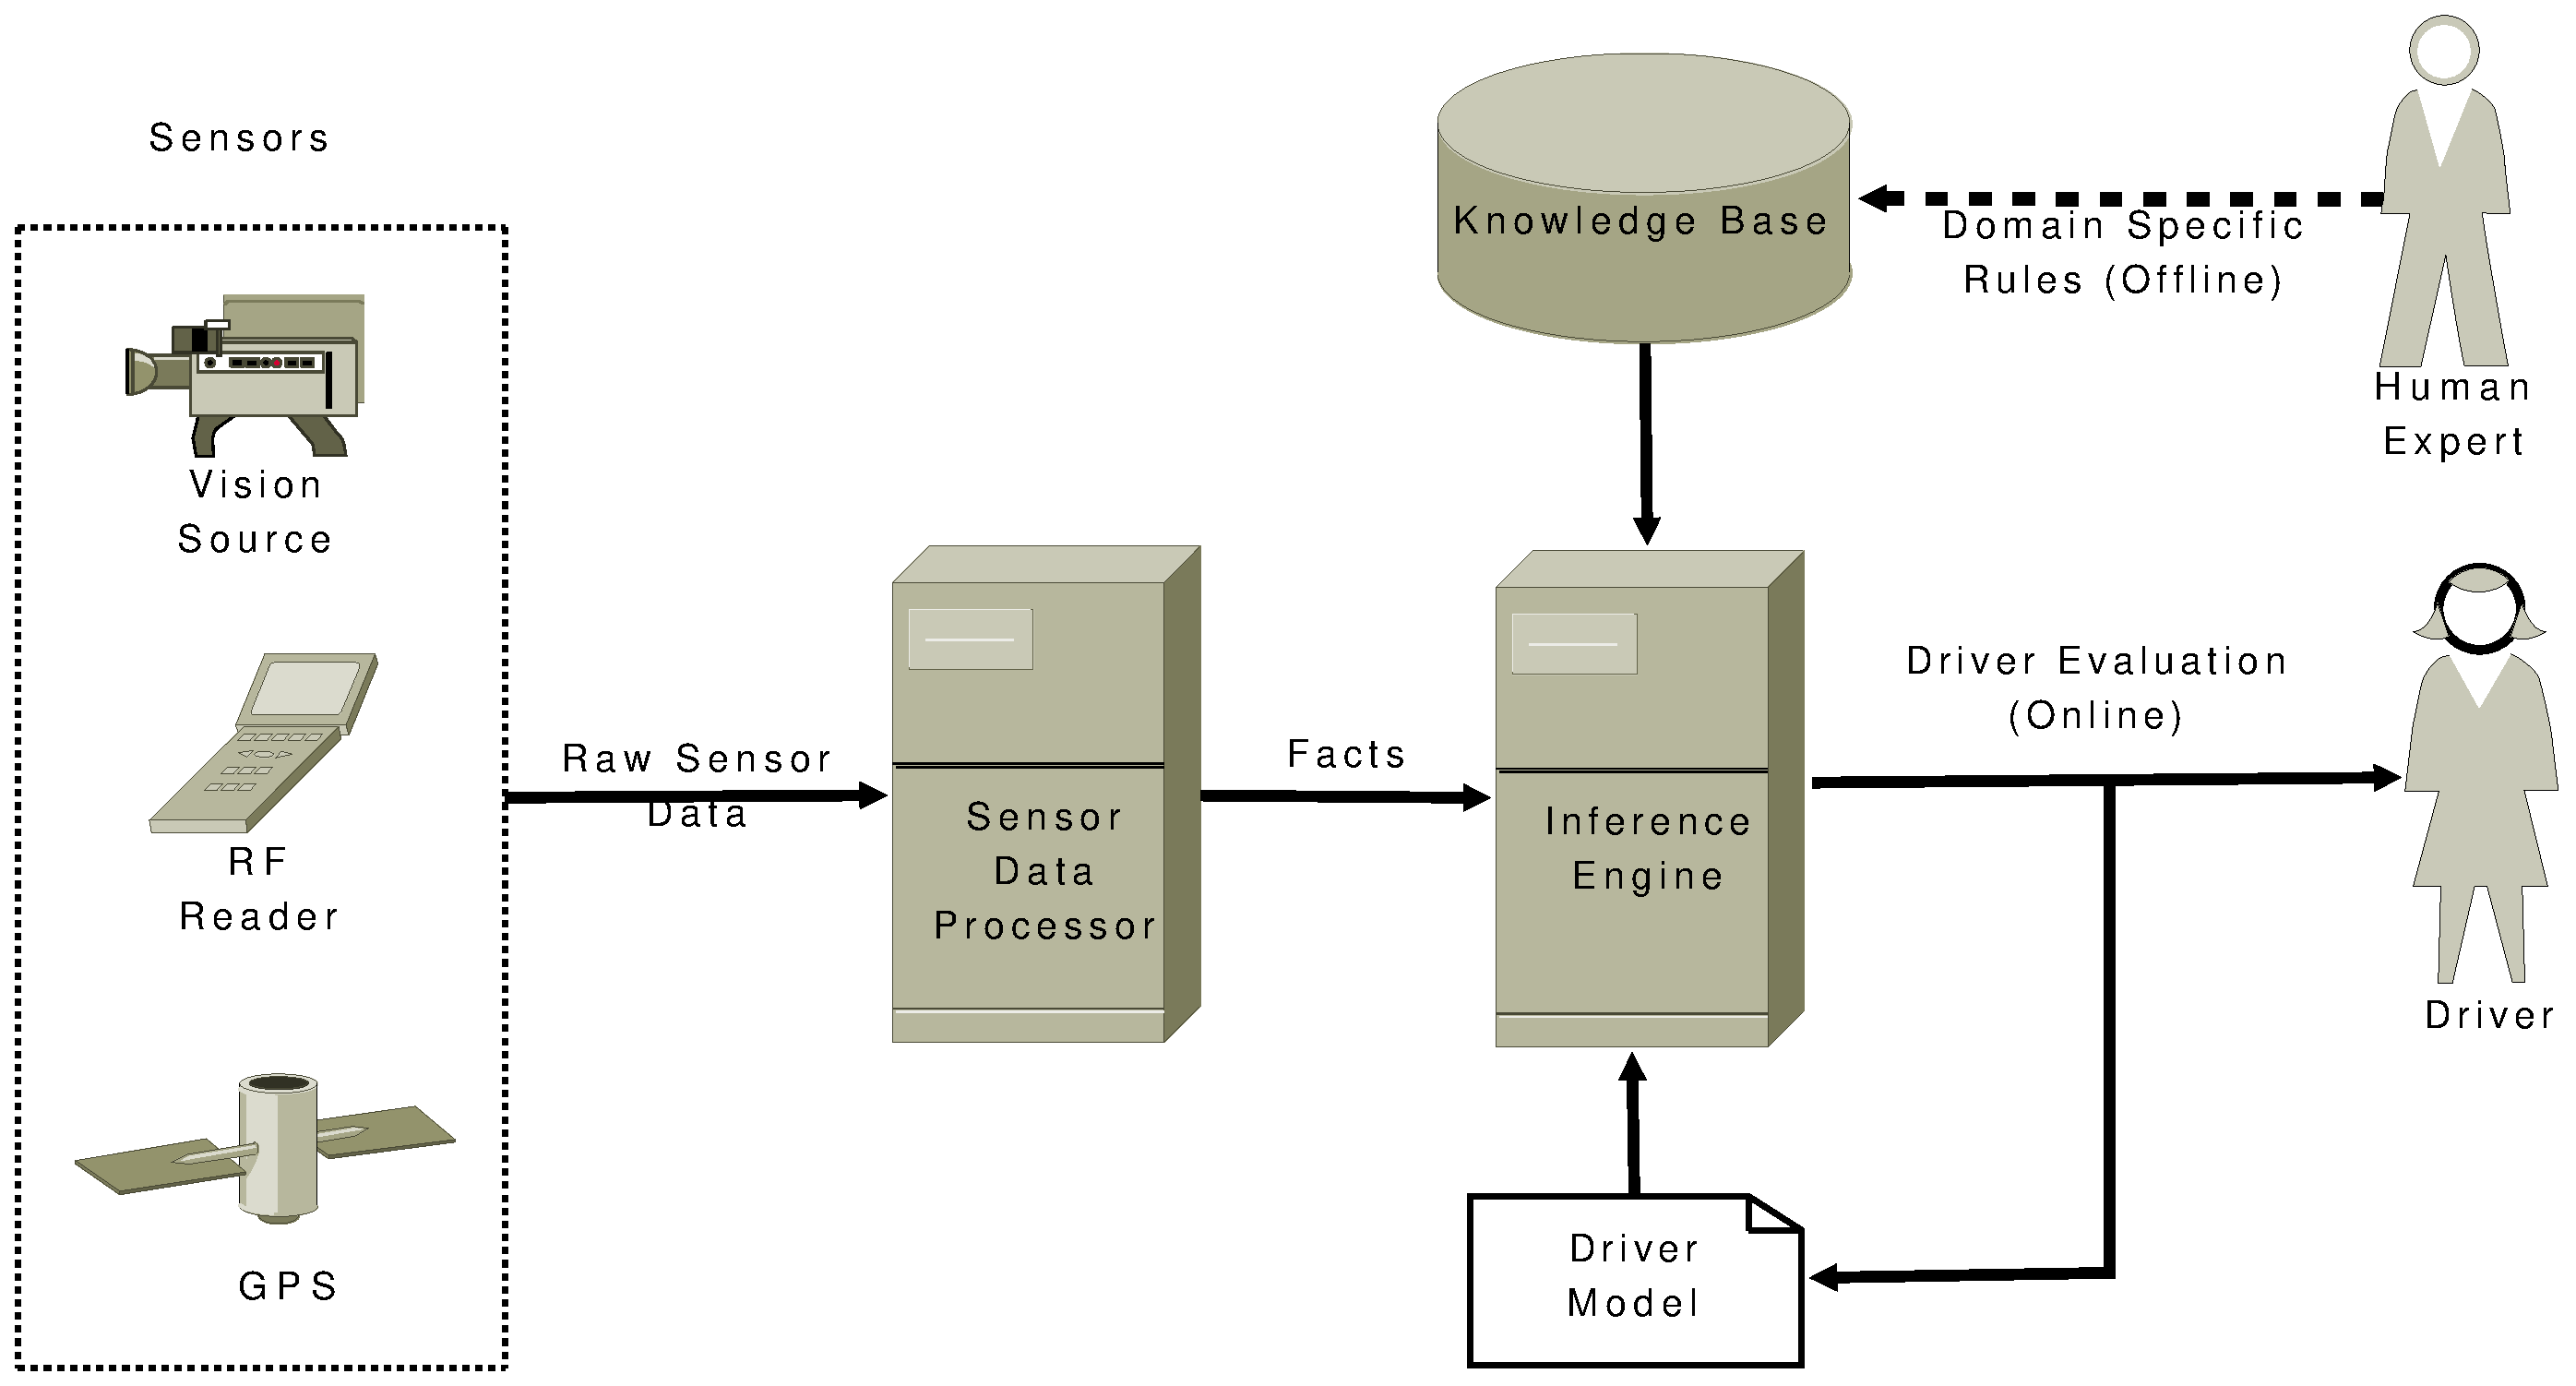
\includegraphics[width=141mm,height=69mm]{img/sys3.eps}
\caption{Basic system architecture of ADES project.}
\label{fig:sys}
\end{center}
\end{figure}

\section{Data Acquisition and Processing}
The most common sensors for mobile agents are video cameras, global navigation satellite systems, light and radio waves based detection and ranging systems. The proposed approach utilizes a single video camera which is placed in the front of the vehicle where the road and other important objects can be seen easily. The RFID technology also inspected in order to reduce the possibility of the errors and increase the reliability of the system. In addition to these modules, there are other commonly used devices for gathering position data and communicating with the vehicle itself.

\subsection{Vision Module}
Since the vision sensors usually provide valuable information about the environment, they are inevitable for most of the autonomous systems. ADES project based on a mono vision sensor, which is a video camera placed on the vehicle. The goal of the vision module is not only capture the image of the environment, but also process this image in order to provide valuable information for the inference engine. The proposed vision processing subsystem will be able to detect and track lane markings and traffic signs. However there are ongoing research projects for detecting traffic lights and various obstacles like other vehicles and pedestrians \cite{shen_robust_2009, gavrila_real-time_1999}.

The set of images includes the defined traffic signs shown in Figure \ref{fig:signs}. The circular ones are regulatory and the triangular ones are the warning signs in Europe ~\cite{ece_revision_2004}. The proposed approach benefits from the red borders which is the most distinct common property of these signs. However, the proposed detection method can be used for different traffic signs in other countries with appropriate fitness functions.

\begin{figure}[ht]
\begin{center}
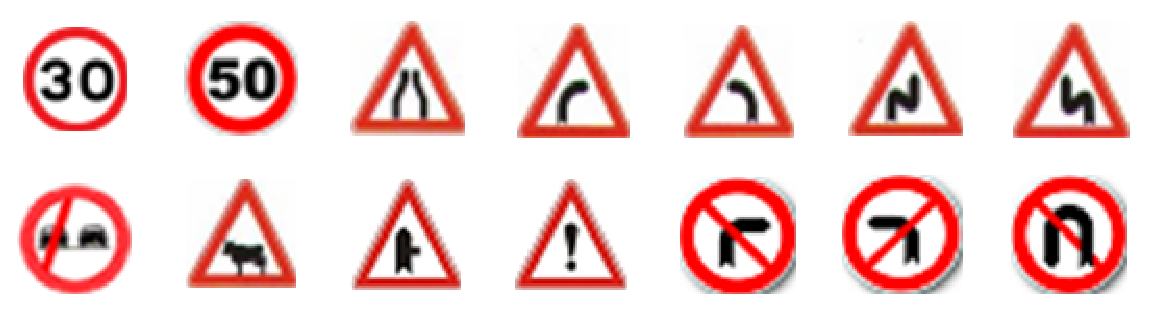
\includegraphics[width=80mm]{img/signs_vertical.eps}
\caption{Traffic signs recognized by the proposed system.}
\label{fig:signs}
\end{center}
\end{figure}
\par

\subsection{RF Module}
In the proposed solution the RF reader is placed within the vehicle due to power requirements. Since the required know-how and resources are beyond the scope of this project, the physical implementation is left as a future work. However, the RF reader and RFID tags are successfully modeled in the simulation environment.

\subsection{Other Sensor Technologies}
There are also other sensors in autonomous driving. One of the most common sensor is RADAR which is a system that uses electromagnetic waves to identify the range, altitude, direction, or speed of both moving and fixed objects. However, more recent applications use the laser scanning radar sensor LIDAR, which measures the relative position of the controlled vehicle with respect to its preceding vehicle. In addition to ranging sensors there are Global Navigation Satellite Systems (GNSS) which uses a version of triangulation to locate the receiver, through calculations involving information from a number of satellites. The most popular GNSS is probably the NAVSTAR GPS, maintained in the United States. There are other systems using satellites as references in the navigation process. Galileo is one GNSS system under development by the European Union (EU). Furthermore, Russia has a system under development called GLONASS \cite{kaplan_understanding_2006}.

\section{Inference Engine} 

The proposed inference system is designed to reason for specific traffic violations. The targeted rules and their fines ~\cite{egm_ceza_2011} are given  Table \ref{ceza}. Although the proposed system is focused on the previous rules, it can also be used for detecting the violations given in Table \ref{ceza2} with necessary improvements like obstacle recognition via vision module or cross-road awareness by GPS.

\begin{table}[ht]
\vskip\baselineskip
\caption{Targeted traffic rules.}
~\vskip -1mm
\centering
% Table generated by Excel2LaTeX from sheet 'tables'
\begin{tabular}{|l|r|}
\hline
{\bf Violation} & {\bf Fine} \\
\hline
Violating the red traffic light &     140 TL \\
\hline
Exceeding speed limits from 10 up to 30 percent &     140 TL \\
\hline
Exceeding speed limits more than 30 percent &     290 TL \\
\hline
Entering forbidden roads. &     140 TL \\\hline
Not obeying the signs and land markings &      66 TL \\
\hline
\end{tabular}    
\label{ceza}
\end{table}

In the current state of the project, there are two expert system implementations which are based on Prolog and Belief Networks. However, any expert system implementation which satisfies specific functionalities, which are detailed in Section \ref{sec:interface}, can be integrated easily to the system.

\begin{table} [ht]
\vskip\baselineskip
\caption{Other relevant traffic rules.}
~\vskip -1mm
\centering
% Table generated by Excel2LaTeX from sheet 'Sayfa1'
\begin{tabular}{|l|r|}
\hline
{\bf Violation} & {\bf Fine} \\
\hline
Not following the rightmost lane unless there is an overriding sign &      140 TL \\
\hline
Following the leading vehicle from an unsafe distance &      66 TL \\
\hline
Not slowing down while entering crossroads, passing hills, crosswalks &      66 TL \\
\hline
Driving too slow or decelerating unexpectedly &      66 TL \\
\hline
Entering the crossroad and blocking the traffic &      66 TL \\
\hline
Not obeying the STOP sign on the school buses &      140 TL \\
\hline
\end{tabular}  
\label{ceza2}
\end{table}
\par



\chapter{METHODOLOGY}
\label{methodology}
The realization of the proposed solution requires implementation and integration of several modules as described in the following sections.
\section{Vision Module}
Vision module is responsible for acquiring raw image data from the camera and processing it to provide information to the expert system implementation. The current implementation is capable of detecting lane markings and specific traffic signs. The overall process is shown in Figure \ref{fig:vision}.
\begin{figure}[ht]
\begin{center}
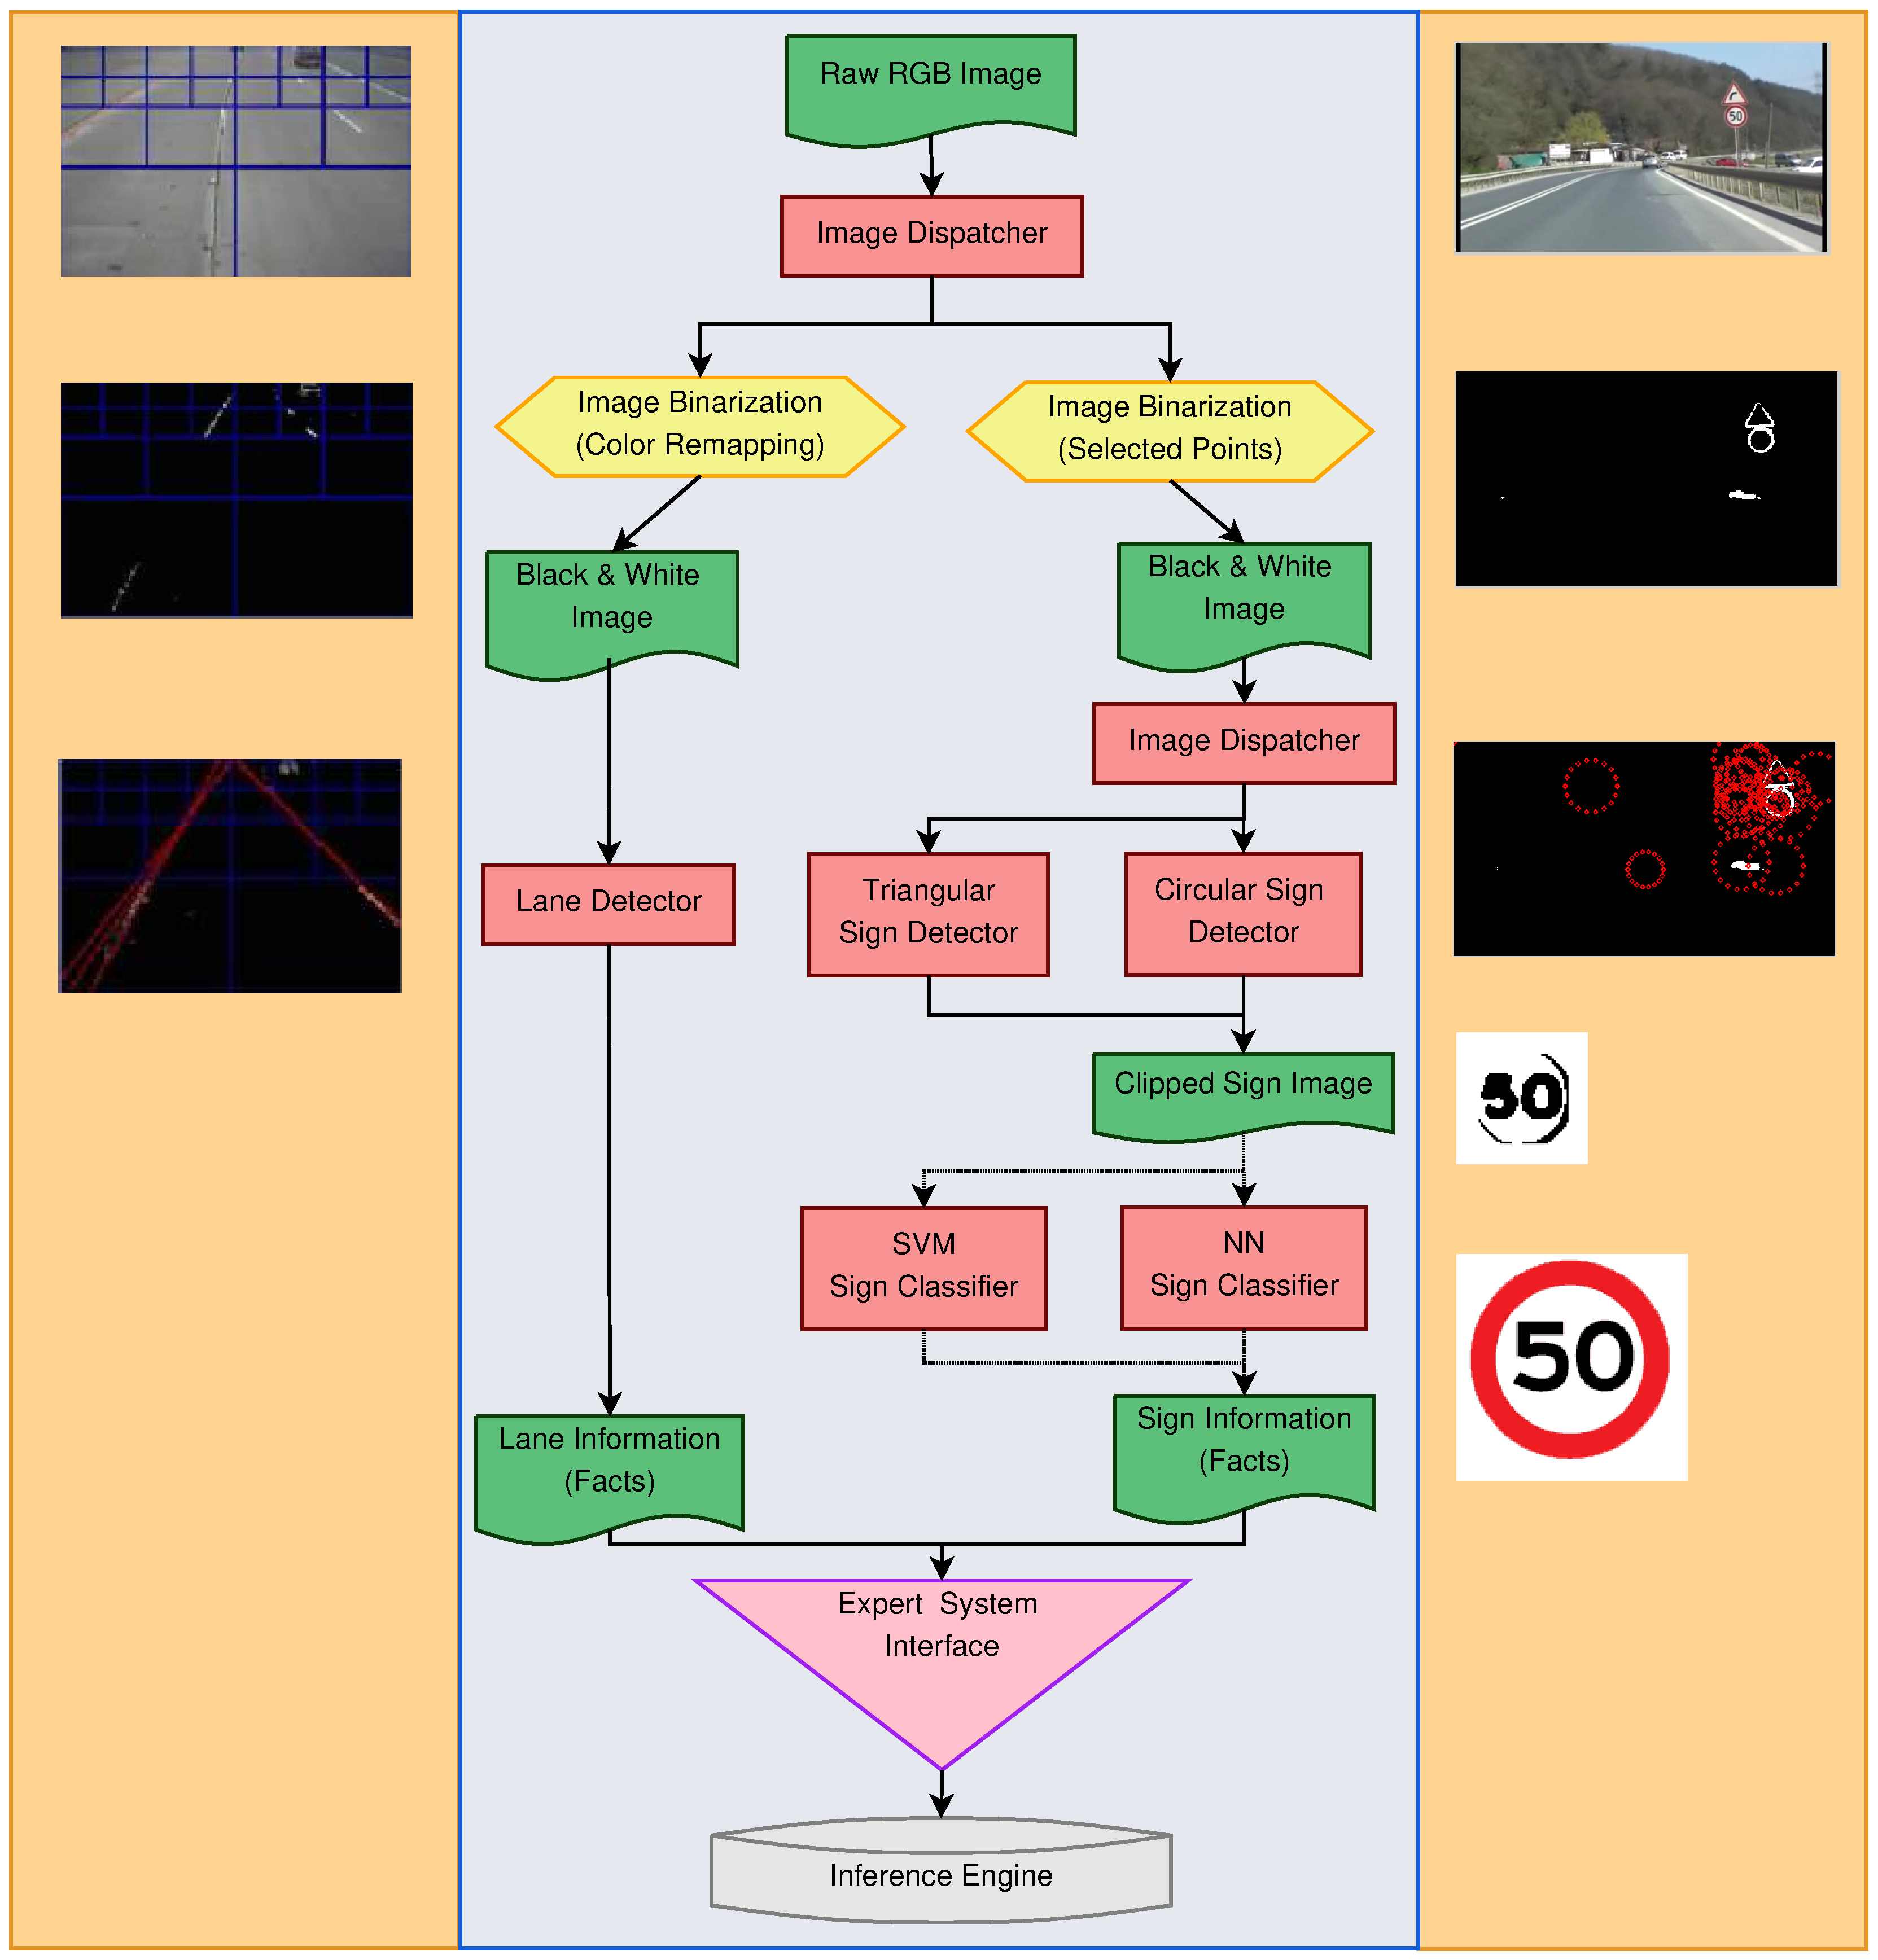
\includegraphics[width=140mm]{img/vision.eps}
\caption{Vision processing.}
\label{fig:vision}
\end{center}
\end{figure}
The entire process is triggered by the arrival of the raw RGB image data. The received image bytes are duplicated for parallel running processes. The first image is preprocessed by a color remapping function to indicate the white and yellow lane markings in the binarized image. The lane detection process then uses this binarized image to find the road lanes. The image binarization process for the sign detection process, however considers the red pixels in the image. The binarized image is duplicated again for the circular and triangular file detection processes. After the location of the traffic sign is detected, the clipped portion of the image is transferred to the predefined sign recognition processor. Currently two sign classification methods are implemented. One of the SVM and NN based sign recognition processors can be selected as desired. The performance of both methods are discussed in Chapter \ref{chapter:evaluation}. Although the current implementation of these classifiers are using grid based features, a Speeded Up Robust Features (SURF) \cite{bay_speeded-up_2008} based feature extraction mechanism is also implemented. The performances of these systems are discussed in the evaluation section.

\subsection{Image Binarization}
The performance of the image binarization process has a dramatic effect on the overall system performance since the remaining processes run on the selected white pixels. If these pixels are not selected properly or incorrectly mapped, the failure of the entire system is guaranteed. In addition, due to the complexity of the detection processes, the binarization process should be very fast for real time applications. Therefore, fast binarization processes with simple but effective mapping algorithms are proposed in this study.

\subsubsection{Color Remapping}
As the first step of the lane detection process, the image is converted to a binary image by using a color remapping function. The mapping for each pixel from the 24bit RGB value to a binary value is given in Table \ref{tabldtable2}. If each mapped value of the red, green, and blue components of the selected pixel is one, then this pixel is a white one in the resulting image. This binarization favors the white and yellow parts of the images. The values have been empirically determined for the video sample. However, for realistic applications an adaptive scenario should be used to accommodate changing lightning conditions.
\begin{table}
\vskip\baselineskip
\caption{Color remapping.}
~\vskip -1mm
\centering
{\footnotesize
% Table generated by Excel2LaTeX from sheet 'tables'
\begin{tabular}{|r|r|r|r|}
\hline
{\bf Pixel Value} & {\bf Red} & {\bf Green} & {\bf Blue} \\
\hline
{\bf 0-176} & 0 & 0 & 0 \\
\hline
{\bf 176-196} & 1 & 1 & 0 \\
\hline
{\bf 196-255} & 1 & 1 & 1 \\
\hline
\end{tabular}  }  
\label{tabldtable2}
\end{table}
\par

\subsubsection{Adaptive Image Binarization}
There are two main image binarization methods proposed for improving the sign detection performance. Both schema try to differentiate the red regions of the image by assigning the most proper values for the coefficients $\alpha$ and $\beta$ in Equation \ref{eq1}.
\begin{eqnarray}
\label{eq1}
f(r,g,b)&=& \left\{\begin{array}{l} 1 \rightarrow r>\alpha \times g, r>\beta \times b \\ 
																		0 \rightarrow o/w \end{array}\right.\\
\nonumber \alpha &>& 1 \\
\nonumber \beta &>& 1
\end{eqnarray}
The mean based image binarization uses the histogram calculations of the acquired frame. Sample scenes with corresponding red, green, blue histograms for 24bit RGB images are given in Figure \ref{fig:hist1}. The values of $\alpha$ and $\beta$ in Equation \ref{eq1} are calculated according to Equation \ref{eq2} where $HSL$ denotes the hue, saturation and lightness histogram arrays.
\begin{figure}[ht]
\begin{center}
\includegraphics[width=60mm,height=60mm]{img/hist1.eps}
\caption{Good, medium and poor conditions for traffic sign detection with corresponding red, green, and blue histograms.}
\label{fig:hist1}
\end{center}
\end{figure}
\begin{figure}

\begin{eqnarray}
\label{eq2}
HIST &=& Histogram(HSL_{rgb}) \\
\nonumber \alpha = \beta &=& 1 + \frac {L_{mean}}{2}
\end{eqnarray}
\end{figure}

However, for sign detection process, the red pixels should be considered. Therefore, in the second approach, the coefficients' values are adjusted according to the total number of white pixels in the binarized image. If the number of the white pixels is less than a predefined value then the coefficients are slightly relaxed. On the opposite side, if there are too many white pixels, then the coefficients are tightened. Since the number of white pixels in the binarized image represents the red-most pixels in the original image, this method is focused on the red pixels of the image.
\begin{figure}[ht]
\begin{center}
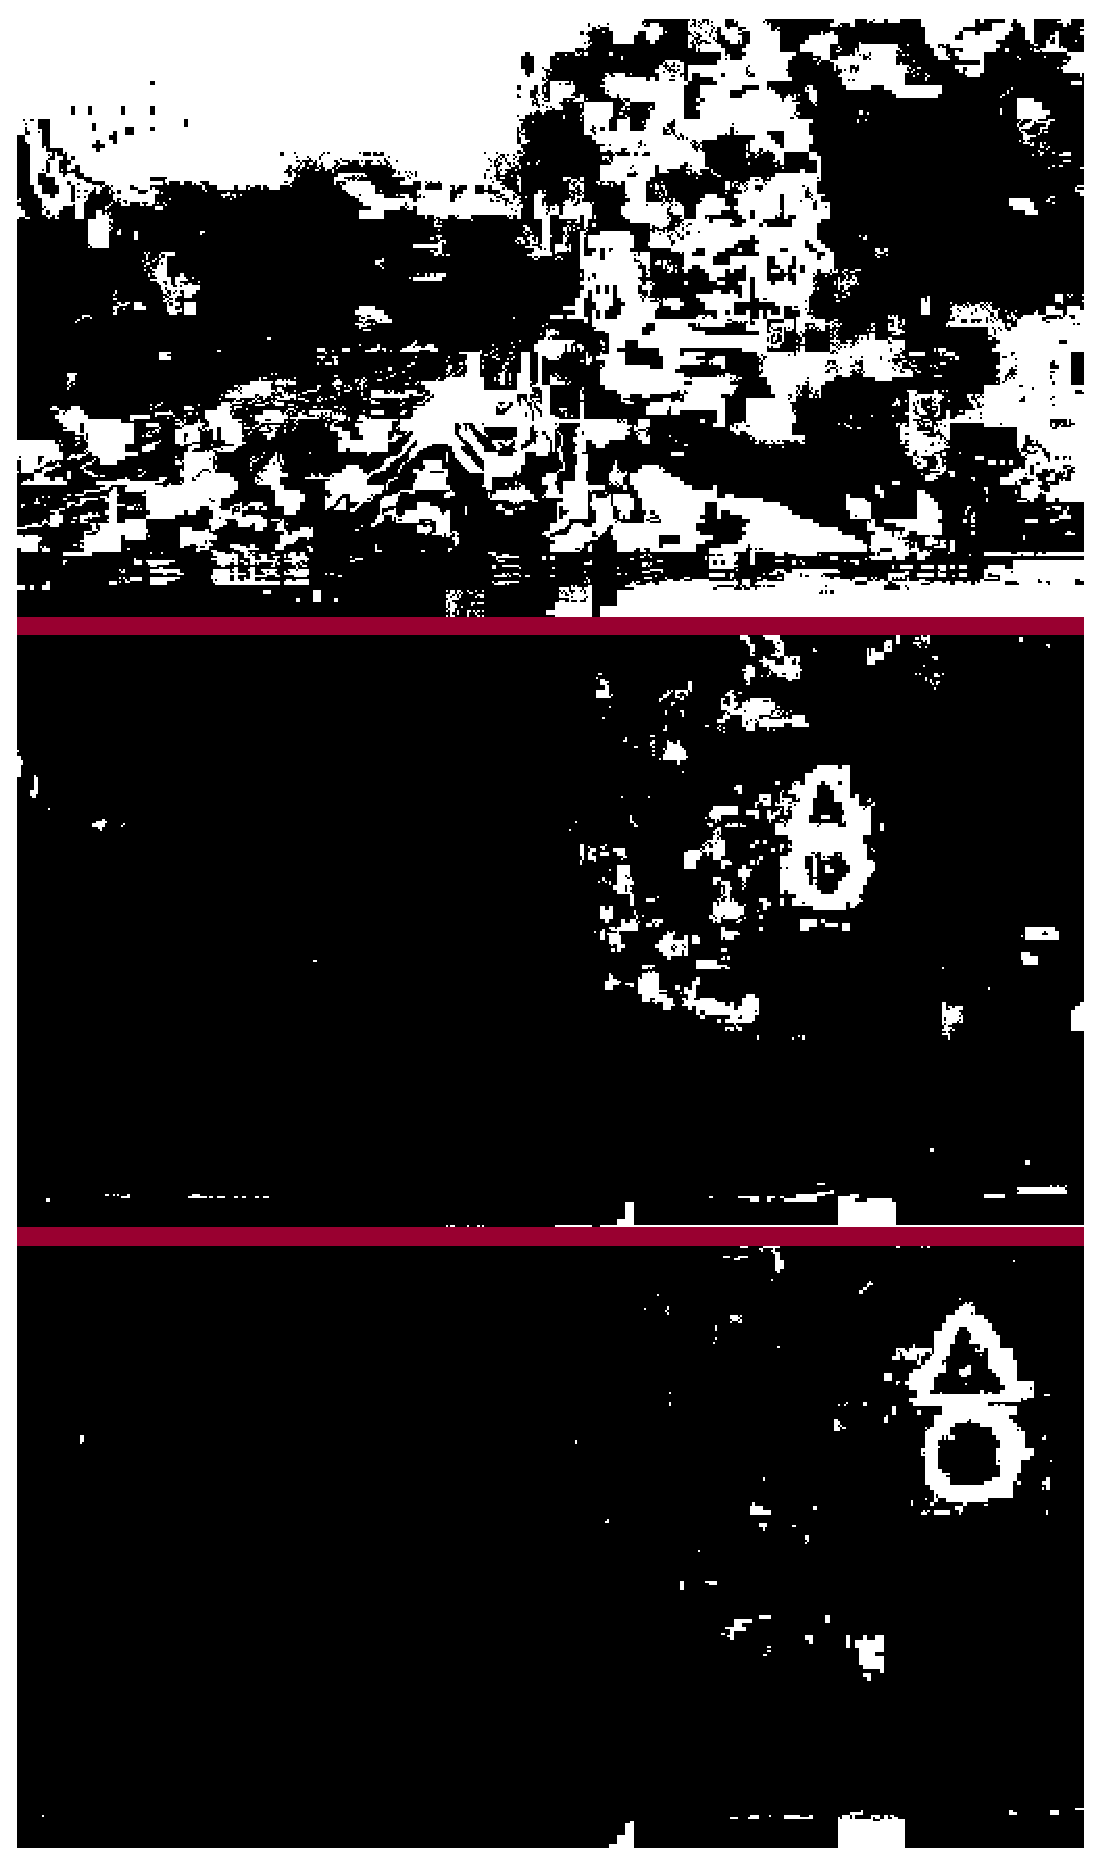
\includegraphics[width=40mm,height=60mm]{img/adapbright.eps}
\caption{Effect of selected point count on image binarization.}
\label{fig:adapbright}
\end{center}
\end{figure}
\begin{figure}

\begin{eqnarray}
\label{eq3}
p_{i} &=& \left\{\begin{array}{l} 1 \rightarrow p=white \\ 0 \rightarrow p=black \end{array}\right.\\
\nonumber p_{white} &=& \sum{p_{i}}, \forall p \in image \\
\nonumber \alpha &=& \left\{\begin{array}{l} \alpha \times \alpha' \rightarrow p_{white}>max_{white} \\ \frac{\alpha}{\alpha'}\rightarrow p_{white}<min_{white} \\ \alpha \rightarrow o/w \end{array}\right., \alpha'>1\\
\nonumber \beta &=& \left\{\begin{array}{l} \beta \times \beta' \rightarrow p_{white}>max_{white} \\ \frac{\beta}{\beta'}\rightarrow p_{white}<min_{white} \\ \beta \rightarrow o/w \end{array}\right., \beta'>1
\end{eqnarray}
\end{figure}

The process can be formulized by Equation \ref{eq3} where $p$ is a pixel on the binarized image. The values of $\alpha'$ and $\beta'$ are usually assigned slightly higher than one (e.g 1.05) to prevent major changes in the consecutive frames. However, the effect of the adaptation is not reduced because of the high frame rate of the streaming media. In Figure \ref{fig:adapbright} the sign becomes clearer as the $\alpha$ and $\beta$ values become 1.02, 1.04, and 1.104 respectively.
\subsection{Road Lane Detection and Tracking}
The classical Hough transformation approach processes the entire vision data in order to detect the lines. This scenario has two main drawbacks. First, the occluded lines (i.e. another car passing through the line) become noisy since the transformed relative intensity of the line decreases. Second, the relative intensity of the lines also decreases at the curves in the road. The proposed solution divides the road image into partitions, where the sizes of the partitions are inversely proportional to the distance of the partition to the vehicle.
\begin{figure}[ht]
\begin{center}
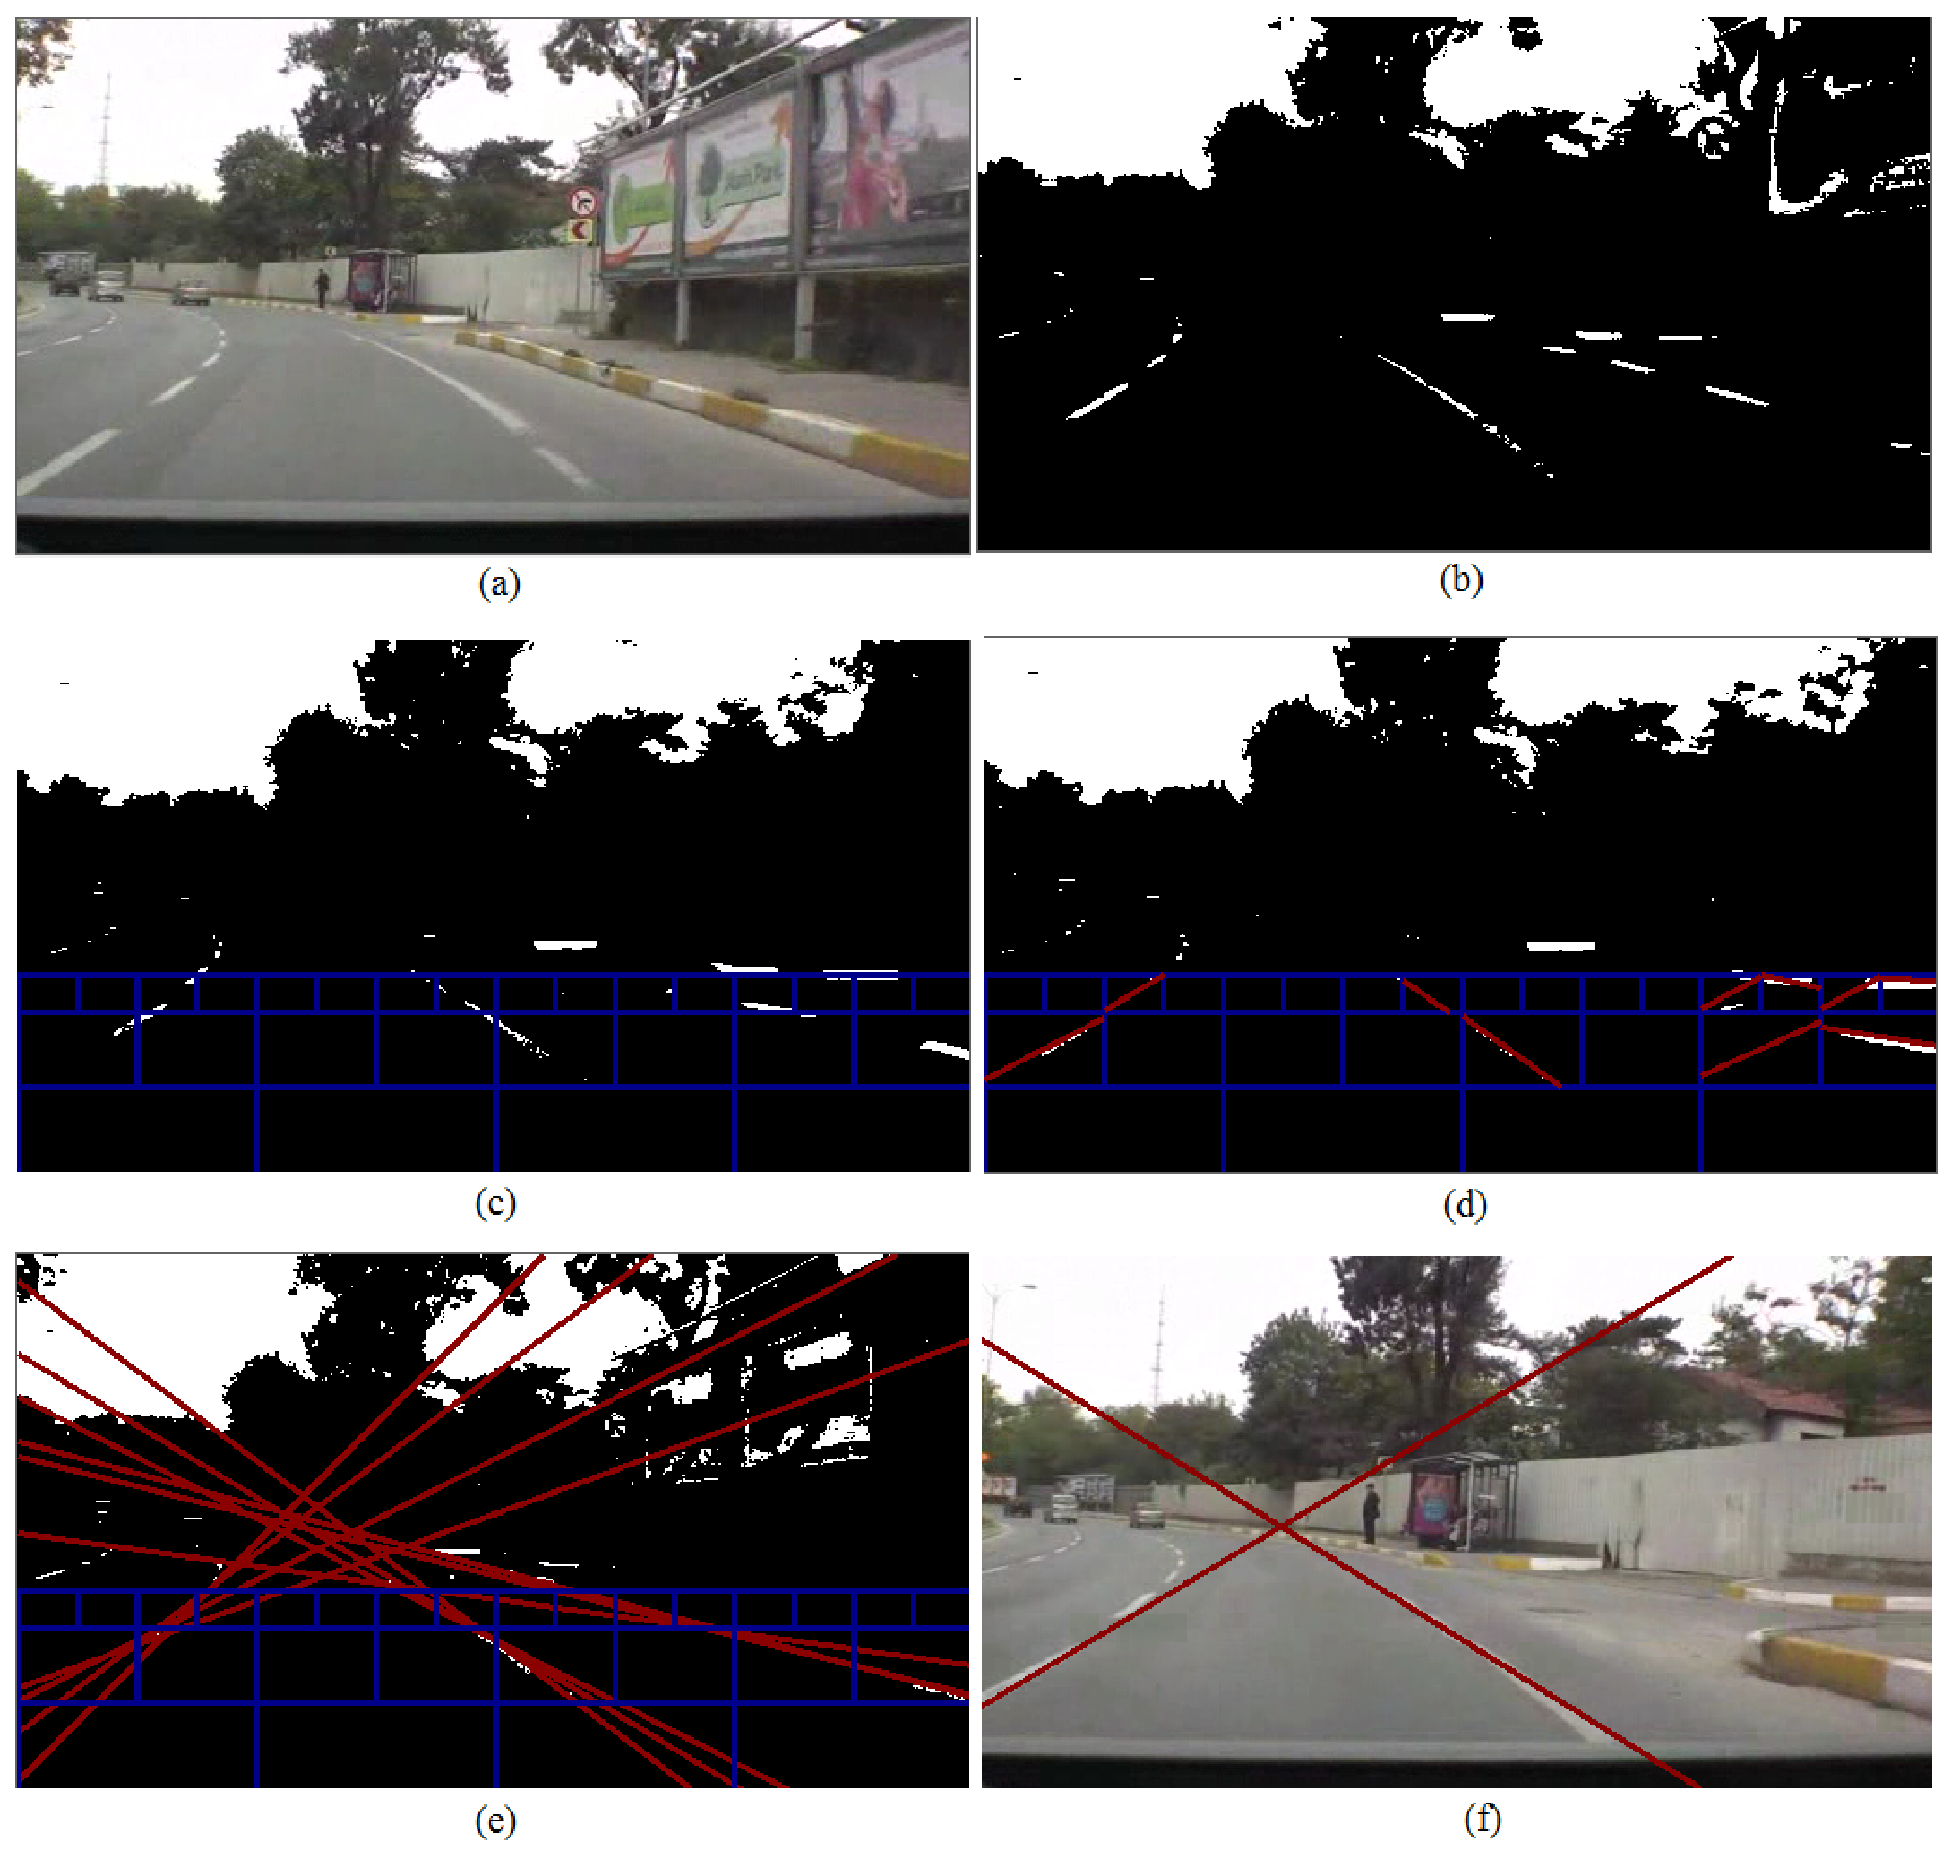
\includegraphics[width=140mm]{img/ldfigmain.eps}
\caption{(a) Original image, (b) Binarized image, (c) Partitions, (d) Hough line segments in partitions, (e) Transformed candidates, (f) Detected lane markings. }
\label{fig:ldfigmain}
\end{center}
\end{figure}
\par
The proposed approach employs Multiresolution Hough Transformation (MHT) for lane detection, followed by two Hidden Markov Process (HMM) models for radius and orientation of the candidate lanes \cite{kaplan_fast_2010}. After the image is partitioned, a separate Hough transformation is applied to each single partition as shown in Figure \ref{fig:ldfigmain}. The most intense line in each partition, which is the candidate line segment, is taken into consideration in order to find the global lanes in the image. Since the Hough lines are represented in polar coordinates \textit{(r, $\theta $)} instead of rectangular coordinates \textit{(x, y)}, the candidate lines are grouped according to their slopes and distances to the center of the image as well as their intensities. The center of the frame is chosen as the bottom most pixel. The transformation of the lines basically changes the center point of the polar coordinates for each transformed line which is achieved by Equation \ref{eq4}
\begin{equation} 
\label{eq4} 
\begin{array}{l} {r'\, \, =\, r+(x-x')\cos (\theta )+(y-y')\sin (\theta )} \\ {\theta '=\, \theta } \end{array} 
\end{equation}
\noindent where \textit{(r', $\theta $')} is the polar coordinates of the transformed Hough line \textit{(r, $\theta $)}. Note that the translation of the center of the Hough transformation is from \textit{(x, y)} to \textit{(x', y')}. 
After the lines are grouped, the most intense three clusters are assigned as the lanes. However, there may be less than three lanes if the sum of the intensities of the candidate lines is less than a threshold value.

For lane tracking, HMM ~\cite{rabiner_introduction_1986} is used to represent the relation between the current frame and its successor. Each line in a specific frame is represented by an individual \textit{(r, $\theta $)} pair. In the succeeding frame, the process will most probably observe the same line at \textit{(r', $\theta $')} which is not very far from the position of the line in the previous frame. The probability of observing \textit{(r', $\theta $')} pair in the next frame is modeled as an HMM problem. In addition, \textit{$\theta $} and $r$ values are modeled by two different HMM. The \textit{$\theta $} value is discretized as (0, 1, 2, 3\dots 178, 179) where the \textit{r} value is discretized at the pixel level. This discretization schema is used for the both transmission and emission matrices. The emission probability matrix shows the probability of observing \textit{$\theta $'} (or \textit{r'}) in the next frame, having observed \textit{$\theta $} (or \textit{r}) in the current frame. In our implementation, the observation and state transition matrix values are derived from two Gaussian distributions with different deviations. The deviation of the transition matrix is assigned to a smaller value than the observation matrix, which means, the state transition matrix aims to preserve the current state where the observation matrix promotes the exploration behavior.

\subsubsection{Implementation Details}
The first step of the implementation is for determining the partitions of the image on which the Hough transforms will be applied. Although the processed sample image is 288 pixels high, only the bottommost 116 pixels are used since the road remains in this lower part of the image. The accuracy of this assumption may slightly differ depending on the slope.
The proposed approach is implemented and tested on a relatively short video sequence of an urban drive. In addition, the new approach is compared with the classical Hough transform where the entire image is processed and the most intense lines are accepted as candidate lines. The properties of the video sequence are given in Table \ref{tab:ldtable1}.
\begin{table}
~\vskip -1mm
\caption{Properties of video sequence.}
\vskip\baselineskip
\centering
% Table generated by Excel2LaTeX from sheet 'tables'
{\footnotesize
\begin{tabular}{|l|r|}
\hline
{\bf Camera Position:} & Front console of the car. \\
\hline
{\bf Resolution:} & 512x288 \\
\hline
{\bf Frame Rate:} & 29.97 \\
\hline
{\bf Length:} & 34 sec. \\
\hline
\end{tabular}  
}
\label{tab:ldtable1}
\end{table}
\par

The widths of the partitions are 32, 64, and 128 pixels from top to bottom, and the heights are 32, 42, and 42 pixels respectively. These values are assigned according to the position of the camera. After the partitions are calculated, Hough transformation is applied to each partition as described in the previous section.  The most promising three lines are assigned as the candidate lane markers. But there may be less than three lines if the intensity of the calculated lines are less than an empirically assigned threshold. The experiments show that the proposed approach usually detects only two lines most of the time. 

After finding the lane markers, HMM method is used to track the lanes. The values of the emission and transition matrices are derived using Gaussian assumption. The deviation of the transition matrix is assigned as 1 and the deviation of the emission matrix is taken as 2. Two separate models are prepared for the \textit{$\theta $} and \textit{r} values of the candidate lane markers. The transition and emission matrices are given in Tables \ref{tab:ldtable3} and \ref{tab:ldtable4}. Since the \textit{$\theta $} values 0 and 179 are actually very close, the emission and transmission values are the same for 1 and 179 in \textit{$\theta $} matrices. In addition, the range of the \textit{r} matrices is (0, 282) because the maximum possible distance for any detected line is 282 pixels where the height of the processed part of the image is 116 and width of the image is 512.

\begin{table}
\vskip\baselineskip
\caption{(a) Transmission matrix for \textit{r}, (b) Transmission matrix for \textit{$\theta $}.}
~\vskip -1mm
\centering
{\scriptsize
\begin{tabular}{|r|r|r|r|r|r|r|r|r|r|}
\hline
{\bf {\normalsize $r$}} & {\bf 0} & {\bf 1} & {\bf 2} & {\bf 3} & ... & {\bf 279} & {\bf 280} & {\bf 281} & {\bf 282} \\
\hline
{\bf 0} & 0,3989 & 0,2420 & 0,0540 & 0,0044 & ... & 0,0000 & 0,0000 & 0,0000 & 0,0000 \\
\hline
{\bf 1} & 0,2420 & 0,3989 & 0,2420 & 0,0540 & ... & 0,0000 & 0,0000 & 0,0000 & 0,0000 \\
\hline
{\bf 2} & 0,0540 & 0,2420 & 0,3989 & 0,2420 & ... & 0,0000 & 0,0000 & 0,0000 & 0,0000 \\
\hline
... & ... & ... & ... & ... & ... & ... & ... & ... & ... \\
\hline
{\bf 280} & 0,0000 & 0,0000 & 0,0000 & 0,0000 & ... & 0,2420 & 0,3989 & 0,2420 & 0,0540 \\
\hline
{\bf 281} & 0,0000 & 0,0000 & 0,0000 & 0,0000 & ... & 0,0540 & 0,2420 & 0,3989 & 0,2420 \\
\hline
{\bf 282} & 0,0000 & 0,0000 & 0,0000 & 0,0000 & ... & 0,0044 & 0,0540 & 0,2420 & 0,3989 \\
\hline
\multicolumn{10}{c}{} \\
\hline
{\bf {\normalsize $\theta$}} & {\bf 0} & {\bf 1} & {\bf 2} & {\bf 3} & ... & {\bf 176} & {\bf 177} & {\bf 178} & {\bf 179} \\
\hline
{\bf 0} & 0,3989 & 0,2420 & 0,0540 & 0,0044 & ... & 0,0001 & 0,0044 & 0,0540 & 0,2420 \\
\hline
{\bf 1} & 0,2420 & 0,3989 & 0,2420 & 0,0540 & ... & 0,0000 & 0,0001 & 0,0044 & 0,0540 \\
\hline
{\bf 2} & 0,0540 & 0,2420 & 0,3989 & 0,2420 & ... & 0,0000 & 0,0000 & 0,0001 & 0,0044 \\
\hline
... & ... & ... & ... & ... & ... & ... & ... & ... & ... \\
\hline
{\bf 177} & 0,0044 & 0,0001 & 0,0000 & 0,0000 & ... & 0,2420 & 0,3989 & 0,2420 & 0,0540 \\
\hline
{\bf 178} & 0,0540 & 0,0044 & 0,0001 & 0,0000 & ... & 0,0540 & 0,2420 & 0,3989 & 0,2420 \\
\hline
{\bf 179} & 0,2420 & 0,0540 & 0,0044 & 0,0001 & ... & 0,0044 & 0,0540 & 0,2420 & 0,3989 \\
\hline
\end{tabular}  
}
\label{tab:ldtable3}
\end{table}

\begin{table}
\vskip\baselineskip
\caption{(a) Emission matrix for \textit{r}, (b) Emission matrix for \textit{$\theta $}.}
~\vskip -1mm
\centering
{\scriptsize
\begin{tabular}{|r|r|r|r|r|r|r|r|r|r|}
\hline
{\bf {\normalsize $r$}} & {\bf 0} & {\bf 1} & {\bf 2} & {\bf 3} & {\bf 4} & {\bf 5} & {\bf ...} & {\bf 281} & {\bf 282} \\
\hline
{\bf 0} & 0,1995 & 0,1760 & 0,1210 & 0,0648 & 0,0270 & 0,0088 & ... & 0,0000 & 0,0000 \\
\hline
{\bf 1} & 0,1760 & 0,1995 & 0,1760 & 0,1210 & 0,0648 & 0,0270 & ... & 0,0000 & 0,0000 \\
\hline
{\bf 2} & 0,1210 & 0,1760 & 0,1995 & 0,1760 & 0,1210 & 0,0648 & ... & 0,0000 & 0,0000 \\
\hline
{\bf 3} & 0,0648 & 0,1210 & 0,1760 & 0,1995 & 0,1760 & 0,1210 & ... & 0,0000 & 0,0000 \\
\hline
{\bf 4} & 0,0270 & 0,0648 & 0,1210 & 0,1760 & 0,1995 & 0,1760 & ... & 0,0000 & 0,0000 \\
\hline
... & ... & ... & ... & ... & ... & ... & ... & ... & ... \\
\hline
{\bf 281} & 0,0000 & 0,0000 & 0,0000 & 0,0000 & 0,0000 & 0,0000 & ... & 0,1995 & 0,1760 \\
\hline
{\bf 282} & 0,0000 & 0,0000 & 0,0000 & 0,0000 & 0,0000 & 0,0000 & ... & 0,1760 & 0,1995 \\
\hline
\multicolumn{10}{c}{} \\
\hline
{\bf {\normalsize $\theta$}} & {\bf 0} & {\bf 1} & {\bf 2} & {\bf 3} & {\bf 4} & {\bf 5} & {\bf ...} & {\bf 178} & {\bf 179} \\
\hline
{\bf 0} & 0,1995 & 0,1760 & 0,1210 & 0,0648 & 0,0270 & 0,0088 & ... & 0,1210 & 0,1760 \\
\hline
{\bf 1} & 0,1760 & 0,1995 & 0,1760 & 0,1210 & 0,0648 & 0,0270 & ... & 0,0648 & 0,1210 \\
\hline
{\bf 2} & 0,1210 & 0,1760 & 0,1995 & 0,1760 & 0,1210 & 0,0648 & ... & 0,0270 & 0,0648 \\
\hline
{\bf 3} & 0,0648 & 0,1210 & 0,1760 & 0,1995 & 0,1760 & 0,1210 & ... & 0,0088 & 0,0270 \\
\hline
{\bf 4} & 0,0270 & 0,0648 & 0,1210 & 0,1760 & 0,1995 & 0,1760 & ... & 0,0022 & 0,0088 \\
\hline
... & ... & ... & ... & ... & ... & ... & ... & ... & ... \\
\hline
{\bf 178} & 0,1210 & 0,0648 & 0,0270 & 0,0088 & 0,0022 & 0,0004 & ... & 0,1995 & 0,1760 \\
\hline
{\bf 179} & 0,1760 & 0,1210 & 0,0648 & 0,0270 & 0,0088 & 0,0022 & ... & 0,1760 & 0,1995 \\
\hline
\end{tabular} 
} 
\label{tab:ldtable4}
\end{table}

\subsection{Traffic Sign Detection and Tracking}
The proposed approach for sign detection and tracking in the ADES project is based on GA and a modified version of radial symmetric transform after an image binarization. 

The GA implementation uses the coefficients of a geometric transformation applied to a set of points which describes the characteristics of any searched template. The formulation of geometric transformation, which includes affine and perspective transformations is given in Equation \ref{eq5}
\begin{eqnarray}
\label{eq5}
\left| \begin{array}{ccc} u' \\ v' \\ w \end{array} \right| &=& 
\left| \begin{array}{ccc} a & b & c \\ d & e & f \\ g & h & 1 \end{array} \right| \left| \begin{array}{ccc} x \\ y \\ 1 \end{array} \right| \\
\nonumber u &=& u'/w \\
\nonumber v &=& v'/w 
\end{eqnarray}
\noindent where $x$ and $y$ are the coordinates of the sample point from the template describing set of points. $u$ and $v$ are the transformed point on the image. $a$, $b$, $d$, $e$  provides rotation, scaling and shearing where $c$ and $f$ used for translation. In addition, $g$ and $h$ provides perspective transformation in two dimensions. These coefficient values or a subset of them can be used in the chromosome encoding of the GA.

The effect of the transformation can be visualized better with a simple example. Assume that $a$, $b$, $c$, $d$, $e$, and $f$ coefficients are used in the encoding of the GA chromosome. In addition, $g$ and $h$ are left zero for simplicity. Also assume that 12 points are used in representing the characteristics of a circular object. For this scenario, we can conclude that a chromosome with the transformation coefficients in Equation \ref{eq6} can yield to the transformed circle points in Figure \ref{fig:sdfig6}. The points on the left hand side of the figure are the characteristic points of the circular template, which are 12 equidistant points on the unit circle, and the right points are the translated, scaled, and rotated counter parties in the transformed domain. 
\begin{eqnarray}
\label{eq6}
\left| \begin{array}{ccc} u' \\ v' \\ 1 \end{array} \right| &=& 
\left| \begin{array}{ccc} 2 & 1 & 100 \\ 1 & 2 & 50 \\ 0 & 0 & 1 \end{array} \right| \left| \begin{array}{ccc} x \\ y \\ 1 \end{array} \right|
\end{eqnarray}
\begin{figure}[ht]
\begin{center}
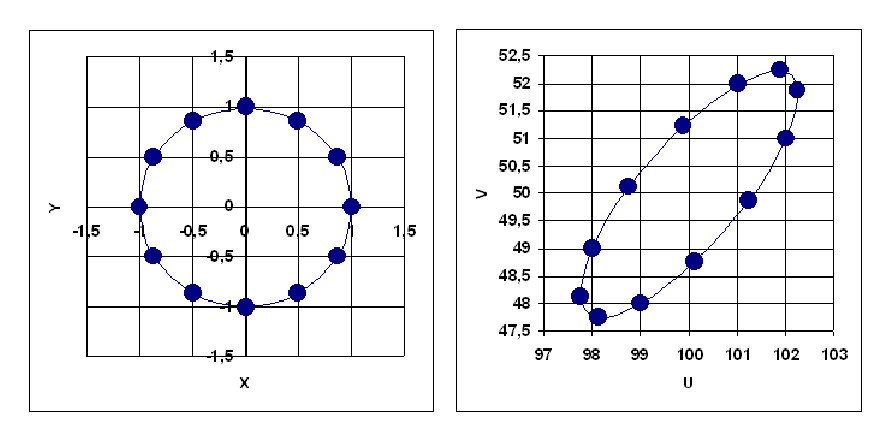
\includegraphics[width=142mm,height=65mm]{img/sdfig6.eps}
\caption{Template characteristic points in $(x,y)$ domain,  and $(u,v)$ domain after the geometric transformation.}
\label{fig:sdfig6}
\end{center}
\end{figure}
\par
These new points are used to calculate the fitness of the candidate traffic sign location. The fitness value is formed as a function of the colors of the underlying pixels for each transformed point in the processed snapshot. 
\subsubsection{Implementation Details}
Similar to the lane detection, the sign detection process also starts with an image binarization process. The second step is creating the population for the GA process. The chromosome encoding is based on the coefficients of the geometric transformation matrix as defined in problem statement section. However, for simplicity, only the two translation and one scaling coefficients are included in the chromosome. The resulting transition matrix is given in Equation \ref{eq7}.
\begin{eqnarray}
\label{eq7}
\left| \begin{array}{ccc} u \\ v \\ 1 \end{array} \right| &=& 
\left| \begin{array}{ccc} a & 0 & c \\ 0 & a & f \\ 0 & 0 & 1 \end{array} \right| \left| \begin{array}{ccc} x \\ y \\ 1 \end{array} \right|
\end{eqnarray}
\par
The crossover process is also a function of these coefficient as given in Equation \ref{eq8}.
\begin{eqnarray}
\label{eq8}
\nonumber a_{newchromosome}&=&\alpha.a_{chromosome1}+\beta.a_{chromosome2} \\
c_{newchromosome}&=&\alpha.c_{chromosome1}+\beta.c_{chromosome2} \\
\nonumber f_{newchromosome}&=&\alpha.f_{chromosome1}+\beta.f_{chromosome2} \\
\nonumber 1&=&\alpha+\beta
\end{eqnarray}
Empirically determined parameters of the GA process are as follows,
\begin{itemize}
		\item Population Size: 100
		\item Number of Iterations: 5
		\item Mutation Rate: 0.05
		\item Selection Rate: 0.9
		\item Selection Method: Elitist
\end{itemize}
In addition to these properties, half of the best chromosomes in a frame is transferred to the next frame in order to provide an initial knowledge about the image. Therefore the number of iterations is kept small. The fitness of the chromosome is evaluated according to the color of the transformed point $(u,v)$ on the binary image. If the value of the pixel is one which means it is a red point on the original image, the fitness of the chromosome is increased. However, this method fails for completely red regions, therefore another set of template points are introduced in order to indicate the non-red points on the template. These points are also subject to the transformation. In this implementation these non-red points are selected to place in the inside of the unit circle. For the example in the problem statement section, if we add the non-red points to the Figure \ref{fig:sdfig6} we end up with Figure \ref{fig:sdfig7} where the red points increase the fitness values when they are white in the binary image, and the black points increase the fitness value when they are black in the binary image. If the expected color cannot be found then the fitness is decreased for each failed point.
\begin{figure}[ht]
\begin{center}
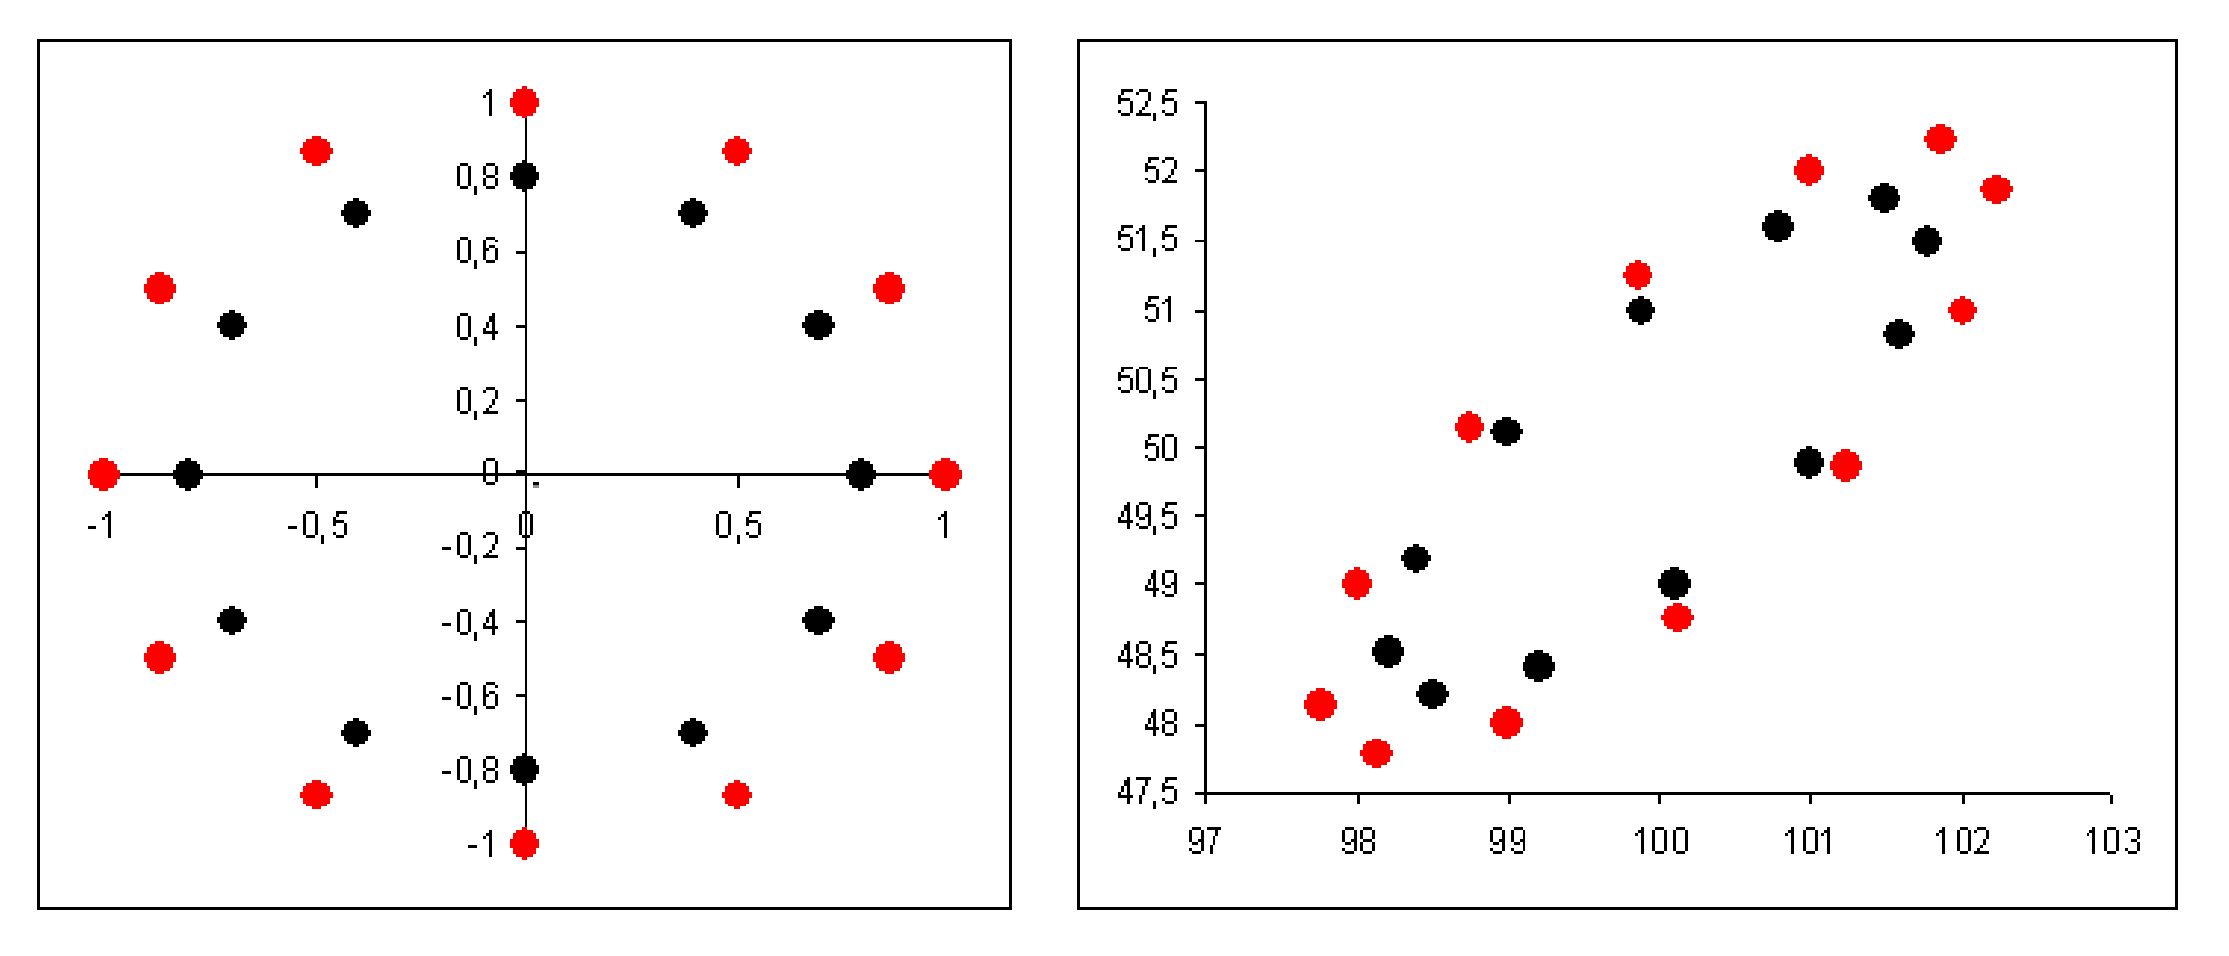
\includegraphics[width=100mm,height=35mm]{img/sdfig7.eps}
\caption{Red and non-red template points.}
\label{fig:sdfig7}
\end{center}
\end{figure}
\par
At each iteration the fitness values are calculated for each chromosome and at the end of the process the chromosomes are expected to converge around the circular sign as shown in Figure \ref{fig:sdfig4}
\begin{figure}[ht]
\begin{center}
\includegraphics[width=60mm,height=35mm]{img/sdfig3.eps}
\includegraphics[width=60mm,height=35mm]{img/sdfig4.eps}
\caption{Initial and converged chromosomes.}
\label{fig:sdfig4}
\end{center}
\end{figure}
\par
Finally if the best chromosome has a fitness value greater than a threshold value, then the points of this chromosome should be on a circular traffic sign on the original image as shown in  Figure \ref{fig:sdfig5}. This complete process takes nearly 50 milliseconds when it is executed on the same hardware specified in Chapter \ref{chapter:evaluation}.
\begin{figure}[ht]
\begin{center}
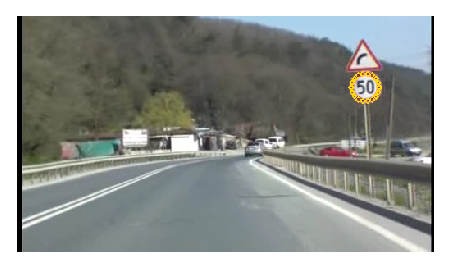
\includegraphics[width=60mm,height=35mm]{img/sdfig5.eps}
\caption{Detected traffic sign.}
\label{fig:sdfig5}
\end{center}
\end{figure}
\par
\subsection{Traffic Sign Classification System}
After the detection phase, the detected image should be classified to provide the sign information to the inference engine. In the ADES project, three different methods are proposed for this purpose.
\subsubsection{Grid Based Neural Network Implementation}
\begin{figure}[ht]
\begin{center}
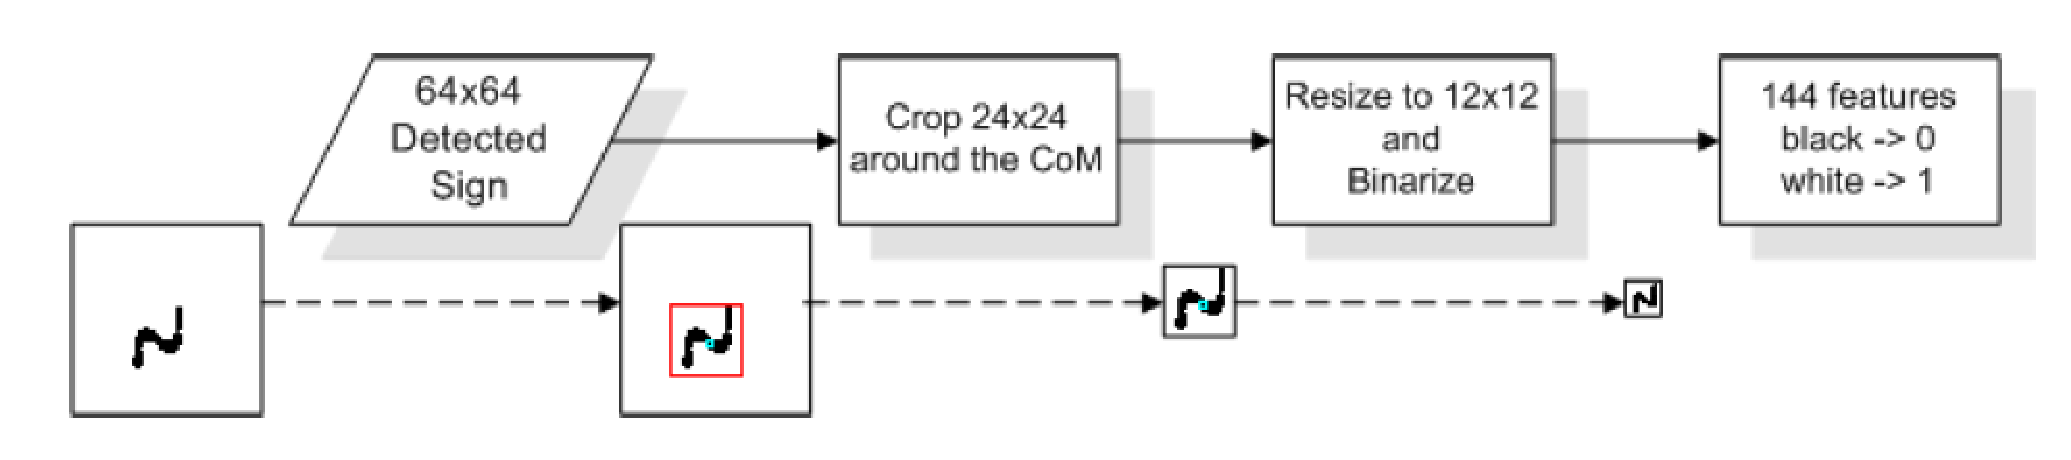
\includegraphics[width=140mm,height=30mm]{img/nn12.eps}
\caption{Input array formation for Grid based NN and SVM implementations.}
\label{signfig23}
\end{center}
\end{figure}
The detected sign is serialized to a binary input array with 144 items where each item is an input for the classifier network as shown in Figure \ref{signfig23}. In the current implementation, each sign has its own network, i.e. the network trained in order to classify that sign, with 144 inputs, 4 hidden layers and one output layer. The networks are trained by using Levenberg-Marquardt learning technique \cite{wilamowski_efficient_1999} which based on solving Equation \ref{eq9}
\begin{eqnarray}
\label{eq9}
	(J^{t}J + \lambda I)\phi &=& J^{t}E
\end{eqnarray}  
\noindent where $J$ is the Jacobian matrix for the system, $\lambda$ is the Levenberg's damping factor. $\phi$ is the weight update vector which is usually found by solving this equation using LU Decomposition. $E$ is the error vector containing the output errors for each input vector used on training the network. The $\phi$ tell us by how much we should change our network weights. The $J^{t}J$ matrix can also be known as the approximated Hessian. The $\lambda$ damping factor is adjusted at each iteration according to the difference in error.

\subsubsection{SURF Based Neural Network Implementation}
SURF \cite{bay_speeded-up_2008} is a scale and rotation invariant feature detector approach. It is basically derived from SIFT \cite{lowe_object_1999} but outperforms it in terms of speed, robustness and distinctiveness. SURF has several parameters that may affect its output:
\begin{itemize}
    \item Upright: This parameter determines whether to run Upright SURF (U-SURF) or not. U-SURF better fits the horizontal camera cases. It runs invariant of image rotation and therefore consumes less CPU time.
    \item Octaves: The scale space is divided into a number of octaves. The filter size is affected by the octave levels.
    \item Intervals: This is the sampling interval. Together with the number of octaves, it determines the number of filters to be applied. (Number of filters = octaves $\times$ intervals)
    \item Threshold: A threshold value used to control the accuracy of the results. Increasing the threshold value will decrease the number of detected interest points.
\end{itemize}
The SURF process finds a set of interest points, which have the following properties.
\begin{itemize}
    \item $(x, y)$: The center of the SURF interest point.
    \item Orientation: This is the orientation of the detected feature in radians. 
    \item Scale: Scale takes values from 1 up to the number of octaves.
    \item Laplacian: A value of 1 indicates bright blobs on dark backgrounds, and -1 indicates just the reverse case.
\end{itemize}
In the early implementations of the project, the neural network was fed by the properties of a constant number of SURF interest points. However, this schema suffers from the ordering of the inputs of the network. Therefore a new schema, which uses the number of SURF points found in predefined parts of the detected image as the input of the network, was developed. \cite{kurtul_road_2009}.

\subsubsection{SVM Implementation}
SVM \cite{cortes_support-vector_1995} models were originally defined for the classification of linearly separable classes of objects. For any particular set of two-class objects, an SVM finds the unique hyperplane having the maximum margin. The solution to a classification problem is represented by the support vectors that determine the maximum margin hyperplane. SVM can also be used to separate classes that cannot be separated with a linear classifier. In such cases, the input values are mapped to a high-dimensional feature space in which the two classes can be separated with a linear classifier. Since the feature space is high dimensional, the nonlinear mapping is computed with special nonlinear functions called kernel. Kernels have the advantage of operating in the input space. The solution of the classification problem is a weighted sum of kernel functions evaluated at the support vectors. 
\par
In our implementation, we used the same input values, which are generated according to the process in Figure \ref{signfig23} to train the SVM with radial basis kernel function (RBF). The RBF kernel function is given in Equation \ref{eq10}
\begin{eqnarray}
\label{eq10}
	k(u,v) &=& e^{-\gamma \times |u-v|^2}
\end{eqnarray}
\noindent where $k$ is the kernel function which gives the distance between the support vector $u$ and the test point $v$. The coefficient $\gamma$ is found by trying sample values at different exponential scales.
\par

\section{RF Module}
The RF module provides information gathered from the RFID tags which are placed special points on the roads ~\cite{sato_development_2006}. An RFID system consists of an antenna and a transceiver which can read the radio frequency and transfer the information to a processing device (reader) and a  transponder, or RF tag, which contains the RF circuitry and information to be transmitted.  The antenna provides the means for the integrated circuit to transmit its information to the reader that converts the radio waves reflected back from the RFID tag into digital information that can then be passed on to computers that can analyze the data. The most common types of RFID modules and specific properties are given in Table \ref{tab:rfid1} ~\cite{finkenzeller_fundamentals_2010}.

\begin{table}[ht]
\vskip\baselineskip
\caption{Properties of most common RFID systems.}
~\vskip -1mm
\centering
{\scriptsize
\begin{tabular}{|r|r|r|r|r|}
\hline
{\bf Band} & {\bf Low Frequency} & {\bf High Frequency} & {\bf Ultra-High Frequency} & {\bf Microwave} \\
\hline
{\bf Typical RFID Frequencies} & 125-134 kHz &  13.56 MHz & 433, 865-956 MHz &   2.45 MHz \\
\hline
{\bf Read Range} &     \textless 0.5m &     \textless 1.5m &       \textless 5m &      \textless 10m \\
\hline
{\bf Data Transfer Rate} &   1 kbit/s &  25 kbit/s & 30-100 kbits/s & \textless 100 kbit/s \\
\hline
{\bf Sample Application} & Car Immobilizer & Contact-less travel cards &  Logistics & Electronic toll collection \\
\hline
\end{tabular} 
}
\label{tab:rfid1}
\end{table}
\par
\subsection{Challenges of RFID Technology}
Although the RFID technology is a commonly used technology especially when fast identification is necessary, it has several challenges for the proposed application \cite{finkenzeller_fundamentals_2010}. 
\begin{itemize}
	\item Power consumption: The most important constraint of the RFID systems is the required power. If the tags are passive, then only the RF reader requires the power. However, for active tags, both the reader and the tags should be connected to a power source. Since the power requirement of the tags are relatively less, they can be equipped with small size batteries. On the other hand, the reader usually requires more power because it provides the current for the antenna. 
	\item Reading range: After the power is supplied to the system, the reading distance of the reader system is calculated according to the structure and positioning of the antenna. Since the proposed application requires omnidirectional reading within two or three meters, the system may require additional amplifiers and power source. In addition, the passive tag solutions are not applicable to the proposed system because of their very low reading distances.
	\item Antenna: The antennas in the current active tag applications are usually designed for static implementations. Therefore the size and the shape of these antennas may result in more complicated designs for the RFID system on the vehicles.
	\item Metal interference: Although there are RFID systems which are not affected from rain or other weather conditions, most of these systems are sensitive to metal interference. The reason of this interference is the reflection and cancellation of the reader's electromagnetic field by metallic objects other than the transponder within the tag.
	\item Passive tag limitations: The passive tags are cheap, easy to place and replace, and require no power source. They are the best candidates for identifying the traffic signs and other important objects. However, the required reading distance by the proposed solution is not available with the current readers without additional equipments. In addition, the limited power source on the vehicle also reduces the performance of the reader system.	
\end{itemize}
\subsection{Tag ID Assignment}
\label{sec:tagid}
The implementation of the RFID technology for the proposed application will contain a reader which is capable of reading tags up to two meters. If the RF reader can be placed somewhere near the front bumper, this distance is sufficient for reading the necessary markings. If we consider the directional restrictions, we place an RFID tag very close to the related regulation sign. In order to detect the violation of the restriction, another RFID tag is also placed a few meters ahead the crossroad in the restricted direction. According to this setup, the system can easily conclude that the driver violates the traffic rule if the RF reader on the car detects the first RFID tag  and then the second tag in this specific order. 

A slightly different scenario can be applied for the traffic lamps. However this time the first RFID tag should be an active one which is activated only when the red light is on. The violation of traffic rule can be detected in the same way as it is done in the previous scenario. The easiness of producing similar scenarios for different traffic rules makes the RFID technology very promising for the ADES project. 

However, to accomplish these scenarios a predefined tag identification number assignment strategy should be designed. In Table \ref{tagid} the tag ID assignment strategy for ADES project is given. In this strategy the RF tags are identified by their global positions, referring traffic rule ids. Finally a redundancy check field is also added for robustness. Since the total number of byte required for indicating a specific rule is eight, several rules can be included within a single tag. This strategy reduces the required number of total tags and the cost of the system.

\begin{table}[ht]
\vskip\baselineskip
\caption{Tag ID assignment strategy.}
~\vskip -1mm
\centering
{\footnotesize
\begin{tabular}{|r|r|r|r|}
\hline
{\bf Tag Part} & {\bf Length (Bytes)} & {\bf Explanation} & {\bf Example} \\
\hline
  UniqueID &          4 & Latitude and Longitude & 41.013144-29.081244 \\
\hline
    RuleID &          1 & Predefined Rule ID & 13 (no trun left) \\
\hline
Pre/Post/Single &          1 & Type of Tag & Pre - no turn left \\
\hline
Matching Tag ID &          1 & Matching Tag for pre/post tags  & UniqueID of pre tag for a post tag \\
\hline
       CRC &          1 & Redundancy Check &   01010101 \\
\hline
           & {\bf Total: 8 bytes} &            &            \\
\hline
\end{tabular} 
}
\label{tagid}
\end{table}



\section{Usage of GPS/GIS and CAN Bus Integration}
The ADES system includes a simple Geographic Information System (GIS) system design and uses this to retrieve the existing traffic rules at the global position of the vehicle \cite{harmon_design_2003}. The proposed GIS database holds the rules as an XML file. A simple example of this XML file is given in Figure \ref{gisxml}.

\begin{mylisting}
\begin{verbatim}
<?xml version="1.0" encoding="utf-8" ?>
<GIS>
  <NodeProp lat="0,0.04,N" lon="0,0.00,W" rule="1"/>
  <NodeProp lat="0,0.12,N" lon="0,0.00,W" rule="13" 
            type="pre" matching="0,0.12,N:0,0.00,W"/>
  <NodeProp lat="0,0.13,N" lon="0,0.02,W" rule="13" 
            type="post" matching="0,0.12,N:0,0.00,W"/>
</GIS>
\end{verbatim}
\end{list}\caption{Simple GIS XML for ADES.}
\label{gisxml}
\end{mylisting}

The attribute properties are similar to the RF Tag ID assignment strategy given in Section \ref{sec:tagid}. The $lat$ attribute gives the latitude of the definition at a predefined resolution. Similarly the $lon$ attribute presents the longitude. The $rule$ presents the existing rule id for the global position defined by the previous attribute. Since there may be only one definition for a specific rule in the defined position, the combination of the $lat$, $lon$, and $rule$ attributes can be considered as the unique ID of the GIS data. The resolution of the system depends on the precision of the $lat$ and $lon$ attributes. In the given example, each rule is effective in nearly 25 square meters in the simulated environment. The $type$ attribute provides additional information about the rule. Finally the $matching$ attribute provides corresponding rule for pre/post rule pairs.

One other tool which can be used to obtain valuable information from the vehicle is the Control Area Network (CAN) bus integration. The CAN is a serial communications protocol developed by Robert Bosch GmbH. It supports distributed real-time control with a high level of security \cite{bosch_specification_1991}. There are many ADAS applications which uses CAN bus integration for obtaining the sensor readings from the vehicle \cite{navet_controller_1998}.  Although advance statistical analyses can be performed on the information obtained from the CAN bus, it also provides simple information like the speed of the vehicle and sensor readings from throttle, break, and steering control units \cite{wang_intelligent_2004, ulmer_vita-autonomous_1992}.

In the ADES simulation environment the speed of the vehicle is provided to the system via the vehicle itself. This scenario can be realized in real life examples by using the CAN bus integration.

\section{Inference Engine}
Expert system is a computer program that uses knowledge and inference functions to solve problems which requires human expertise for their solution \cite{merritt_building_2001}. The knowledge base and inference rules are either hand coded or learned by the system by observing another expert, possibly a human expert. The most important difference of an expert system from a conventional computer application is its inference engine. As an example, a dictionary may be a conventional computer program where a successful translator can be addressed as an expert system. 
\par
The knowledge base consist of the information encoded in a specific way and the basic functions to deal with this data. The inference engine is the main part of the expert system which uses these functions on available information to come up with a solution. However, an expert system has to explain its solution in a way that an human observer can understand. Moreover, an expert system may also utilize a learning subsystem to update its information and inference capabilities.
\par
The expert system models can be categorized into two categories which are probabilistic and rule based models \cite{castillo_expert_1991}. The major properties of these models and their comparison are shown in Table \ref{tab1} and Table \ref{tab2}.
\begin{table} [ht]
\vskip\baselineskip
\caption{Properties of expert system models.}
~\vskip -1mm
\centering
{\footnotesize
\begin{tabular}{|p{50mm}|p{40mm}|p{40mm}|}
\hline
 & {\bf Probabilistic Model} & {\bf Rule Based Model} \\
\hline
{\bf Knowledge Base} & Probabilistic Structure,  Facts & Rules, Facts \\
\hline
{\bf Inference Engine} & Conditional probability evaluation (Bayes theorem) & Backward chaining, Forward chaining \\
\hline
{\bf Explanation Subsystem} & Based on conditional probabilities & Based on triggered rules \\
\hline
{\bf Learning Subsystem} & Change in probabilistic structure and probabilities & Adding, removing rules \\
\hline
\end{tabular}
}
\label{tab1}
\end{table}

\begin{table}[ht]
\vskip\baselineskip
\caption{Comparison of expert systems models.}
~\vskip -1mm
\centering
{\footnotesize
\begin{tabular}{|p{50mm}|p{40mm}|p{40mm}|}
\hline
 & {\bf Probabilistic Model} & {\bf Rule Based Model} \\
\hline
{\bf Advantages} & Easy learning, Easy probability propagation & Easy explanation, Easy modification \\
\hline
{\bf Shortcomings} & High number of parameters & Performance issues, Certainty implementation \\
\hline
\end{tabular}  
}
\label{tab2}
\end{table}
There are advantages and disadvantages of both models. The probabilistic model provides a proper handling of uncertainty with easy learning capabilities. Statistical information can be used directly to form a probabilistic model. However, high number of parameters even in small models makes the model more complicated to understand and manage. On the other hand, the rule based systems are easier to maintain. However, this advantage usually causes performance issues when extensive rule chaining is required for complex problems.

\subsection{Expert System Interface}
\label{sec:interface}
In order to integrate various expert system implementations into the ADES project, we defined an interface as shown in Fig. \ref{fig:interface}. 

\begin{mylisting}
\begin{verbatim}
public interface ExpertSystems
        {
            string init(params object[] esParams);
            string assertFact(params object[] esParams);
            string retractFact(params object[] esParams);
            string[] query(params object[] esParams);
            void setThreshold(double threshold);
            double getThreshold();
        }
\end{verbatim}
\end{list}\caption{ADES Interface for Expert Systems.}
\label{fig:interface}
\end{mylisting}


The $init$ function initializes the expert system with various parameters like network definition files for BN based expert systems or the built in predicates of the Prolog based expert system. The $assertFact$ function provides the high level information to the expert system. This information is formed by processing the data acquired from different sensors. The $retractFact$ function is used when a previously introduced information is invalidated. However, the expert systems are free to retract their facts according to their internal operations. The $query$ function is the main procedure triggered right after a fact is asserted or retracted. This function is expected to return the kind of violation and its probability if there is a traffic violation. Finally, the $setThreshold$ and $getThreshold$ functions are used for arranging the threshold level of the expert system for deciding a violation. In the current state of the projects there are two implementations of this interface which are the Prolog based and Belief Network's based expert systems.

\subsection{Implementation with Prolog}

Prolog is a programming language for symbolic computation \cite{bratko_prolog_1986}. It is suitable for solving problems which contains objects and relations between these objects. The relations with variables are called the \textit{rules}. Rules have condition and conclusion parts. On the other hand, the \textit{facts} are means of stating that relations exist between objects. Therefore, the relations of the facts only contains atoms \cite{bratko_prolog_1986, sterling_art_1994}. The power of Prolog comes from three major features of the language which are rule-based programming, built-in pattern matching and backtracking execution. Pattern matching and backtracking features provide automatic control of the flow in the program which make it possible to realize many types of expert systems \cite{merritt_building_2001}. 

Writing a Prolog program is not similar to writing a program in a conventional programming language. The Prolog programmer should consider the formal relationships exist in the problem domain. In other words, Prolog approach is more like describing the facts and rules about the problem domain instead of prescribing a procedural algorithm \cite{clocksin_programming_1994}.

\subsubsection{Probabilistic Prolog Enhancement}
In real life problems, the relations between the objects are not always very clear. Therefore, an expert system should also consider the uncertainties associated with the supplied data. There are different ways to provide certainty factors or probabilities to the facts in Prolog. In the simplest way the facts can be coupled with their probabilities as shown in Figure \ref{fig:ppe}.

\begin{mylisting}
Rules and Facts
\vspace*{2pt}\hrule
\begin{verbatim}
weather(fine,P) :- sky(sunny,PS),temp(high,PT),P is PS*PT.
sky(sunny,0.8).
temp(high,0.9).
\end{verbatim}

Query
\vspace*{2pt}\hrule
\begin{verbatim}
?- weather(X,P).
X = fine
P = 0.72 (0,016 sec)
\end{verbatim}
\end{list}\caption{Probabilistic Prolog example.}
\label{fig:ppe}
\end{mylisting}

\noindent In this example, the probability of a fine weather condition is calculated according to the probabilities of the sky and temperature facts with given probability values. This method works well for small examples, however, unnecessary probability calculation overhead in the rules and the additional parameters in the fact definitions can increase the complexity in more complicated applications. 

The second approach use operators to give probabilities to the facts. Unlike the previous examples, the rules do not have additional parameters for probability calculations. We can modify the previous example as shown in Figure \ref{fig:fwo}.

\begin{mylisting}
Rules and Facts
\vspace*{2pt}\hrule
\begin{verbatim}
weather(fine):-sky_sunny,temp_high.
"0.8::sky_sunny".
"0.9::temp_high".
\end{verbatim}

Query
\vspace*{2pt}\hrule
\begin{verbatim}
?- weather(X).
Prob for sky_sunny is 0,8
Prob for temp_high is 0,9
Prob for this answer:0,72
X = fine (0,000 sec)
\end{verbatim}
\end{list}\caption{Facts with operators.}
\label{fig:fwo}
\end{mylisting}

In this project this method is preferred and the probability operator '::' is implemented within the Prolog engine. However, there are other implementations where the probability processing extensions can be consulted as libraries without changing the engine itself \cite{de_raedt_problog_2007}.

Another common example for visualizing the operation of the probabilistic Prolog is the path finding application. In this example a small Prolog application is presented to find a path on a graph. The probability of the achieved path is calculated from the probability values assigned to the  edges of a graph. If the directed graph in Figure \ref{fig:graph} is considered, there are three acyclic path from node one to node five.

\begin{figure}[ht]
\begin{center}
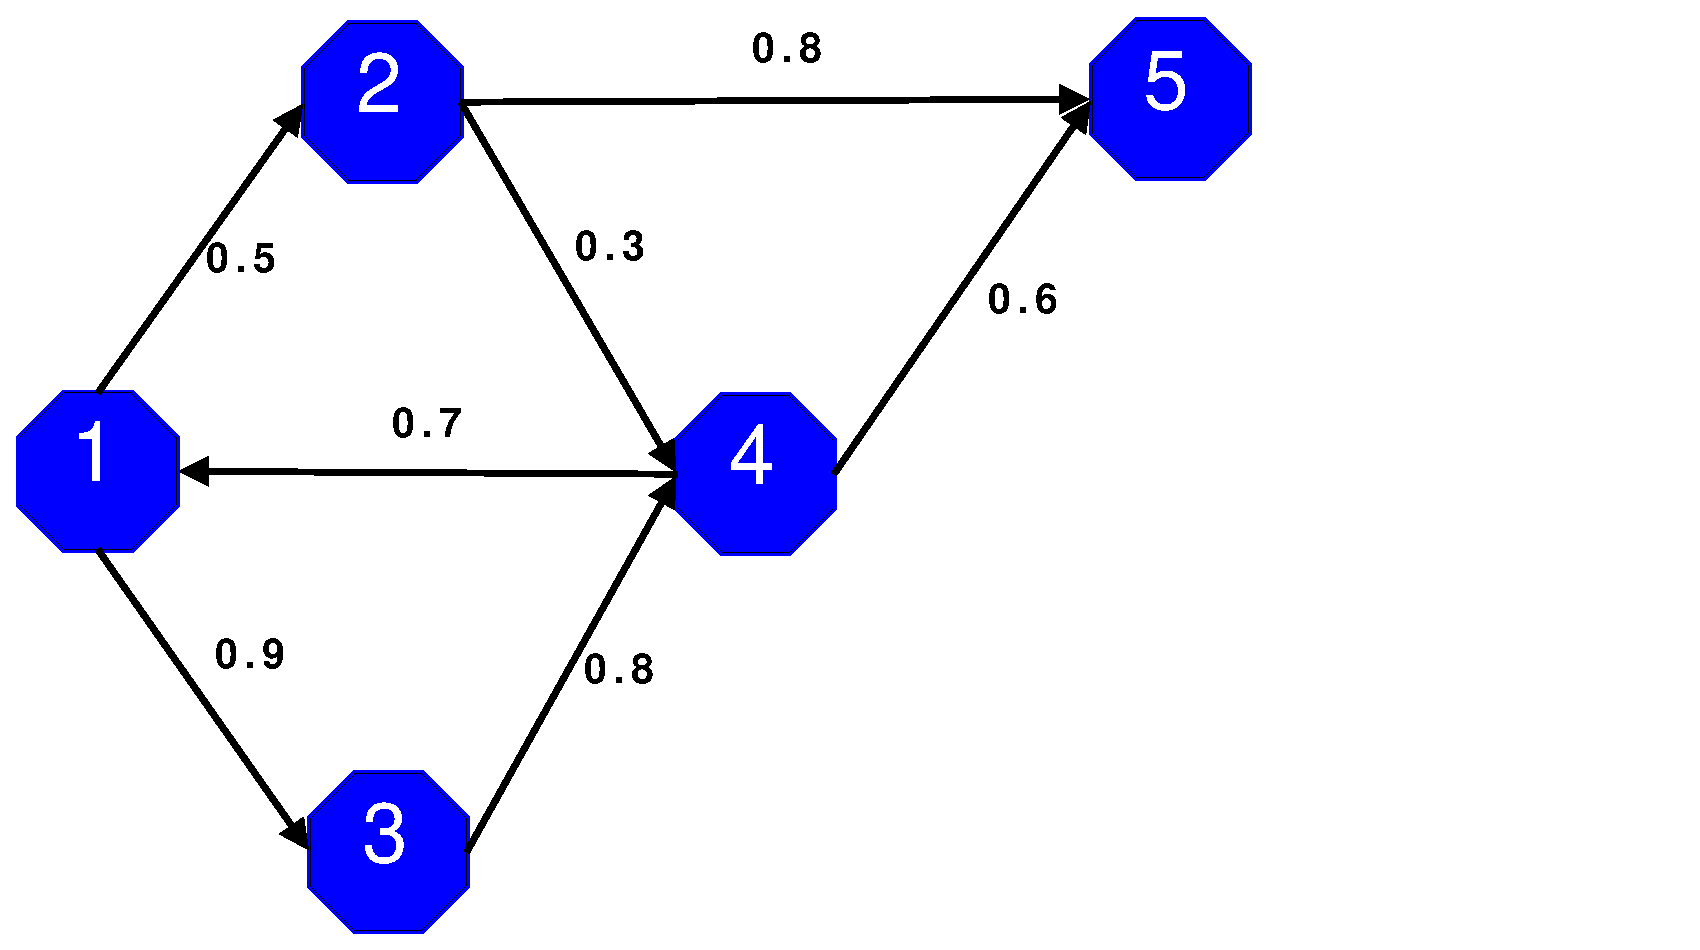
\includegraphics[width=80mm,height=40mm]{img/graph.eps}
\caption{Directed graph with probability values.}
\label{fig:graph}
\end{center}
\end{figure}

The representation of the graph by facts, the Prolog program which returns the paths between two nodes, and the result of a sample query are given in Figure \ref{fig:ppfge}.

\begin{mylisting}
Rules and Facts
\vspace*{2pt}\hrule
\begin{verbatim}
path(X,Y,[X|NL]) :- pathX(X,Y,L), reverse(L,[],NL), notvisited(X,NL).

pathX(X,Y,L) :- pathX(X,Y,_,L).
pathX(X,X,A,A).
pathX(X,Y,A,R) :- X\==Y, edge(X,Z), notvisited(Z,A), pathX(Z,Y,[Z|A],R).

notvisited(X,[Y|Z]):- X \= Y, notvisited(X,Z).
notvisited(_,[]).

reverse([X|Y],Z,W) :- reverse(Y,[X|Z],W).
reverse([],X,X).

"0.9::edge(1,3)".
"0.5::edge(1,2)".
"0.3::edge(2,4)".
"0.8::edge(2,5)".
"0.8::edge(3,4)".
"0.7::edge(4,1)".
"0.6::edge(4,5)".
\end{verbatim}

Query
\vspace*{2pt}\hrule
\begin{verbatim}
?- path(1,5,L).
Prob for this answer:0,432
L = [1,3,4,5] (0,000 sec) more? (y/n);
Prob for this answer:0,09
L = [1,2,4,5] (0,000 sec) more? (y/n);
Prob for this answer:0,4
L = [1,2,5] (0,000 sec) more? (y/n);
no
\end{verbatim}
\end{list}\caption{Prolog program for graph example.}
\label{fig:ppfge}
\end{mylisting}

This program finds a path without traversing a node twice and returns the list of nodes on the path. The algorithm keeps a list of visited nodes which prevents infinite loops on cyclic links. As mentioned before, the rule definitions do not deal with the probability issues, which means they do not have any object, or parameter related with probability calculations. The probability values of the edges are given within the fact definitions.
\subsubsection{Time-Decaying Facts}
Although the probabilistic extension to the Prolog engine provides mechanisms for dealing with uncertainty, the required expert system should possess additional properties. One of these improvements is the time-decaying property of the probabilistic facts. This enhancement is required when the asserted fact has some time limitations. For example, if the sensors indicate that there is a directional restriction on the way, then we may want to assign an expiration time like 30 seconds for that fact. 

The decay function can be any monotonically decreasing one which starts from one and eventually decreases to zero. In the proposed system sigmoid functions are used as the decay function. The characteristic behavior of the sigmoid function, given in Equation \ref{eq11}, is illustrated in Figure \ref{fig:sigmoid} where $\alpha$ is 0.5 and $\beta$ is 30. According to this function the probability of the given fact will halve within 30 seconds, and the fact will retracted from the database before 45th second. It is clear that the decaying characteristics can be easily controlled by modifying the $\alpha$ and $\beta$ parameters.

\begin{equation}
\label{eq11}
f(x) = 1- \frac{1}{1+e^{\alpha\times(\beta-x)}}
\end{equation}

\begin{figure}[ht]
\begin{center}
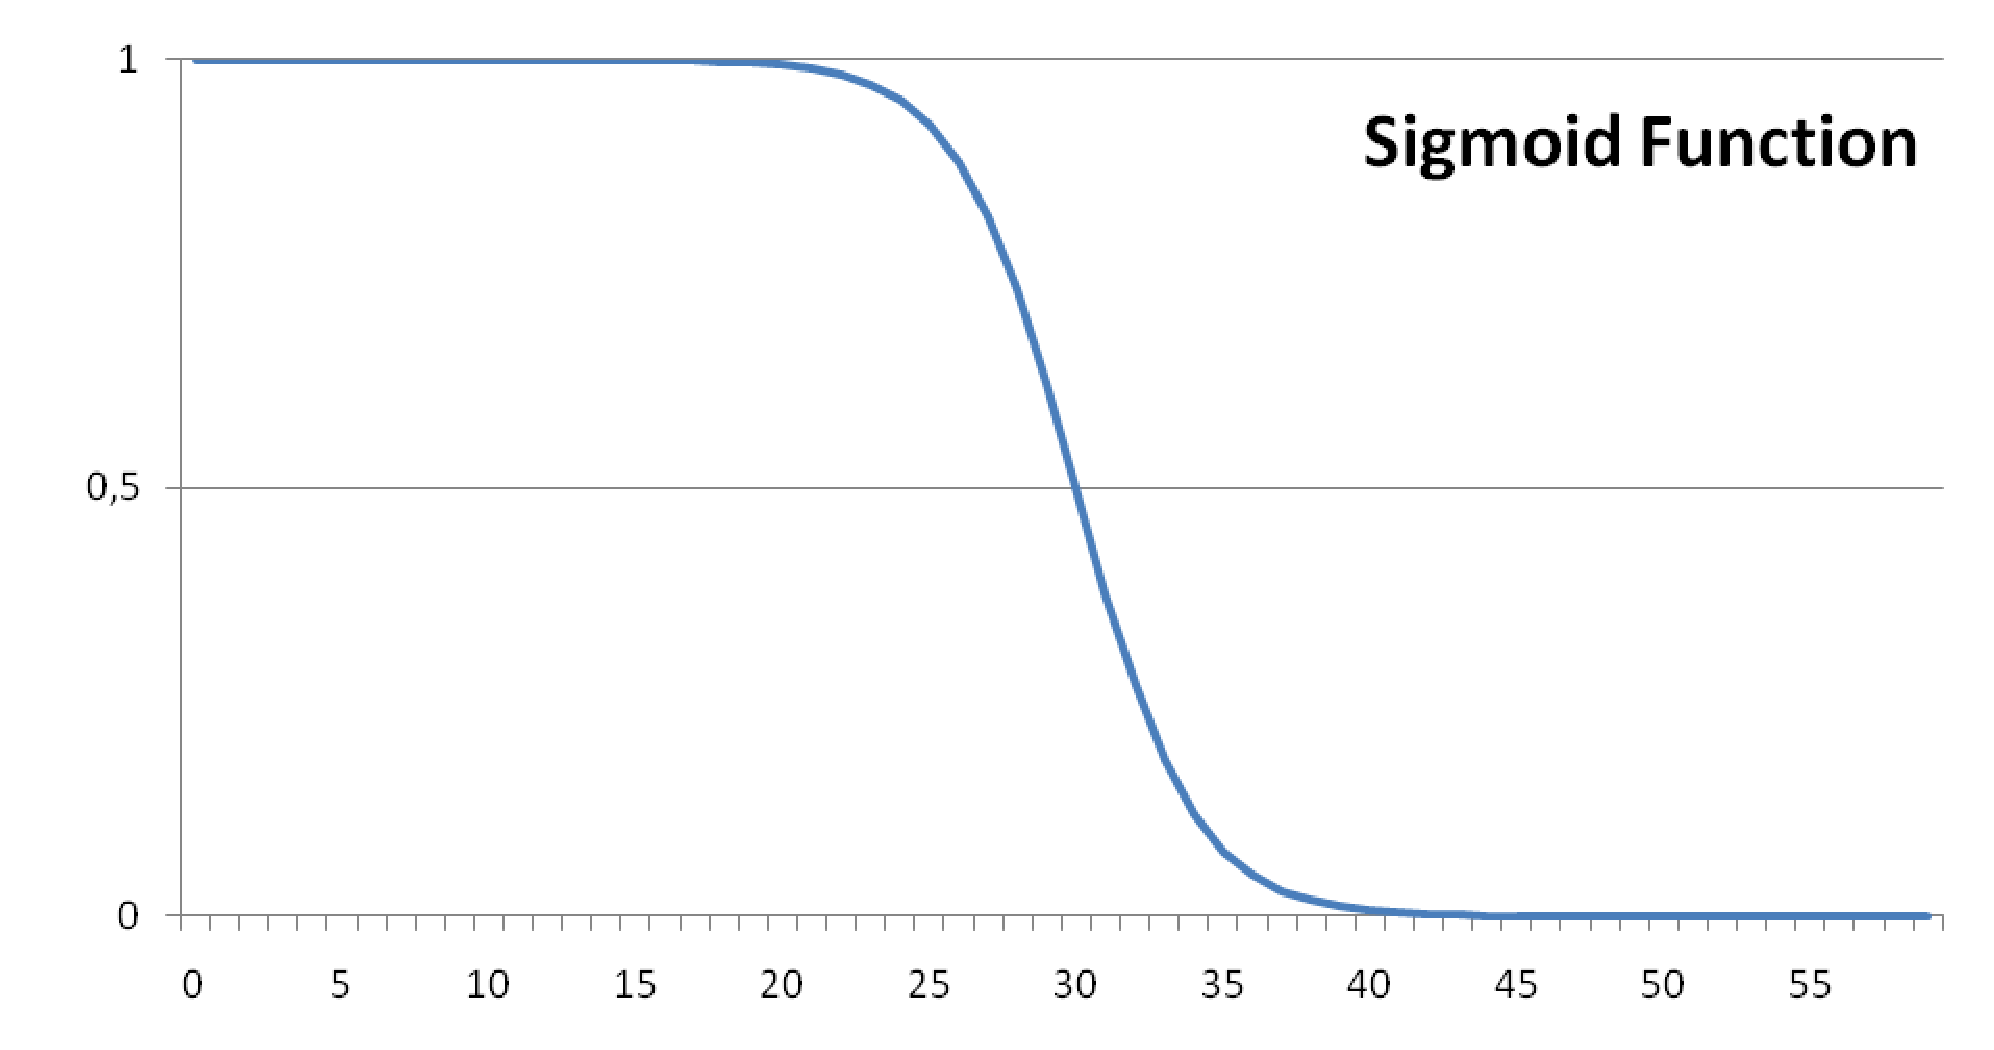
\includegraphics[width=80mm,height=40mm]{img/sigmoid.eps}
\caption{Sigmoid function used for time-decaying facts.}
\label{fig:sigmoid}
\end{center}
\end{figure}

The time-decaying property of the facts are given in their definitions. In the previous graph example, assume that the probability of the edge between second and fourth nodes is decreasing over time. According to our sigmoid function, the probability of this edge becomes 0.15 at 30th second after the fact is asserted. And finally the fact will no longer be available after 45 seconds as shown in Figure \ref{fig:tdf}.

\begin{mylisting}
Rules and Facts
\vspace*{2pt}\hrule
\begin{verbatim}
%only replace the fact about edge(2,4)
%remaining facts and rules are the same...
"0.3::T::edge(2,4)".
\end{verbatim}

Query
\vspace*{2pt}\hrule
\begin{verbatim}
%initial response to the query
?- path(2,4,L).
Prob for this answer:0,299999908226781
L = [2,4] (0,000 sec) more? (y/n);
no

%waiting for 30 seconds
?- path(2,4,L).
Prob for this answer:0,155176213884928
L = [2,4] (0,000 sec) more? (y/n)
no

%after 45 seconds
?- path(2,4,L).
no
\end{verbatim}
\end{list}\caption{Time decaying facts.}
\label{fig:tdf}
\end{mylisting}
The $T$ literal between two probability operators '::' indicates that the probability of the fact will decay according to the built-in decay function, which is the sigmoid function in the proposed implementation. An integer value can also be placed instead of the $T$ value to enlarge or shorten the duration of the value as shown in the Figure \ref{fig:gewtdf}.

\begin{mylisting}
Rules and Facts
\vspace*{2pt}\hrule
\begin{verbatim}
%replace T value with -20 to speed up the decay process
"0.3::-20::edge(2,4)".
\end{verbatim}

Query
\vspace*{2pt}\hrule
\begin{verbatim}
%initial response to the query
?- path(2,4,L).
Prob for this answer:0,299999908226781
L = [2,4] (0,000 sec) more? (y/n);
no

%waiting for 10 seconds
?- path(2,4,L).
Prob for this answer:0,155176213884928
L = [2,4] (0,000 sec) more? (y/n)
no

%after 25 seconds
?- path(2,4,L).
no
\end{verbatim}
\end{list}\caption{Graph example with time decaying facts.}
\label{fig:gewtdf}
\end{mylisting}

\subsection{Implementation with Belief Networks}

A belief network (BN) is an acyclic graph used for modeling the uncertainty in a domain \cite{pearl_fusion_1986}. The nodes of the graph are random values and the arcs are conditional dependencies between these variables. BN's are reasoning tools that depend on the laws of probability. Although it is possible to design multiply-connected (or cyclic) BN's, probabilistic inference using this type of networks is NP-hard \cite{cooper_computational_1990}.

The BN based expert system developed for the ADES project uses discrete random variables represented by a singly-connected graph. The value of a discrete random variable should be a member of the discrete values from a finite set of states. In addition, the sum of the probabilities of those states for each variable should be equal to one.

\subsubsection {Microsoft Bayesian Network Editor}
The Microsoft Bayesian Network Editor \\
\noindent (MSBNx) is a Microsoft Windows library for creating and evaluating Bayesian Networks \cite{kadie_msbnx:_2001}. It can be used as a standalone modeling and inference application, or the run-time components which provide Bayesian reasoning services can be integrated to custom applications. The graphical interface for developing BN graphs can be used in both cases. The resulting BN files can be consulted by the custom application during run-time. The main purpose of MSBNx environment is diagnostic and troubleshooting inference using complicated evidences.

In the ADES project, MSBNx is used for implementing the BN expert system. The networks are created by using the MSBNx editor. These networks are loaded to the application when the application initializes. 


When BN is selected as the active expert system, in case of an arrival of information, the probabilities of the states in the initial nodes are arranged according to the certainty of the information. After this arrangement, all of the loaded networks are queried for a possible violation. The networks respond to this inquiry by returning their derived beliefs for the \textit{YES} state of the violation variable. The belief of this state highly depends on the subjective probabilities entered by experts.

\subsection{Regulation Implementations}
In the ADES Project, the goal is to detect the traffic violations according to the sensor values. The proposed inference engine includes rules for detecting the violations given in Table \ref{viol} to accomplish this mission.
\begin{table}[!ht]
\vskip\baselineskip
\caption{Targeted traffic violations.}
~\vskip -1mm
\centering
{\tiny
\begin{tabular}{|r|r|c|}
\hline
&&\\
{\scriptsize No Turn Left} & 
\includegraphics[scale=0.3]{img/noleft} & {\scriptsize Sign Detection,}\\
&&\\
\cline{1-2}
&&\\
{\scriptsize No Turn Right} & 
\includegraphics[scale=0.3]{img/noright} & {\scriptsize RFID Detection,}\\
&&\\
\cline{1-2}
&&\\
{\scriptsize No U Turn} & 
\includegraphics[scale=0.3]{img/nouturn} & {\scriptsize GPS/GIS Information,}\\
&&\\
\cline{1-2}
&&\\
{\scriptsize No Entrance} & 
\includegraphics[scale=0.3]{img/noenter} & {\scriptsize Vehicle Speed,}\\
&&\\
\cline{1-2}
&&\\
{\scriptsize Speed Limit} & 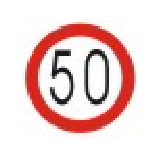
\includegraphics[scale=0.3]{img/speedlimit} & {\scriptsize Steering Angle,} \\
&&\\
\cline{1-2}
&&\\
{\scriptsize No Overtaking} & 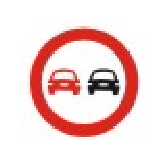
\includegraphics[scale=0.3]{img/overtake} & {\scriptsize Lane Detection,}\\
&&\\
\cline{1-2}
&&\\
{\scriptsize Traffic Lights} & 
\includegraphics[scale=0.3]{img/trafficligt} & {\scriptsize Time Elapsed}\\
&&\\
\hline
\end{tabular}  
}
\label{viol}
\end{table}
The assertion and retraction of each fact triggered from the sensors are given in Table \ref{assert}. It is the responsibility of the expert system to keep the facts up to date according to these rules. The speed of the vehicle is not included in the table because it is retracted and asserted again by the system before each validation query.

\begin{table}[!ht]
\vskip\baselineskip
\caption{Assertion and retraction of the facts.}
~\vskip -1mm
\centering
\label{assert}
{\footnotesize
% Table generated by Excel2LaTeX from sheet 'Sayfa1'
\begin{tabular}{|r|l|l|}
\hline
{\bf Regulation} & {\bf Assertion of Facts} & {\bf Retraction of Facts} \\
\hline
Directional & Traffic sign detection & After a period of time. \\
\cline{2-3}
           & GPS node rule from GIS & Exiting the node. \\
\cline{2-3}
           & RFID tag detection (Pre/Post) & After a period of time, \\
\cline{3-3}
           &            & Detecting another RFID tag for the same rule. \\
\hline
     Speed & Traffic Sign Detection & Restriction ends sign detection, \\
\cline{3-3}
           &            & Another speed limit sign. \\
\cline{2-3}
           & RFID tag detection & After detecting another RFID tag for the same rule. \\
\cline{2-3}
           & GPS node rule from GIS & Exiting the node. \\
\hline
Traffic Lights & GPS node rule from GIS & Exiting the node. \\
\cline{2-3}
           & RFID tag detection (Pre/Post) & Detecting another RFID tag for the same rule. \\
\hline
Illegal Overtake & Traffic sign detection & Restriction ends sign detection. \\
\cline{2-3}
           & GPS node rule from GIS & Exiting the node. \\
\cline{2-3}
           & Solid Lane Departure & Immediately after query. \\
\hline

\end{tabular}  
}
\end{table}

In the following sections the explanations of these rules are given. In the expert system design, it is assumed that the inference engine acquires data from three sensor systems which are the vision system, the RFID system and the GPS system. Additional systems can be introduced to the application as long as they can provide facts to the inference engine with their certainty factors. 

\subsubsection{Violation of Directional Regulations}
The directional regulations considered in our application are `no turn left', `no turn right', `no U turn', and `no entrance' conditions. For detecting such violations, inputs from the vision, the RFID and the GPS systems are utilized in the proposed rule. A sample scenario is illustrated in Figure \ref{fig:dirreg}.

\begin{figure}[ht]
\begin{center}
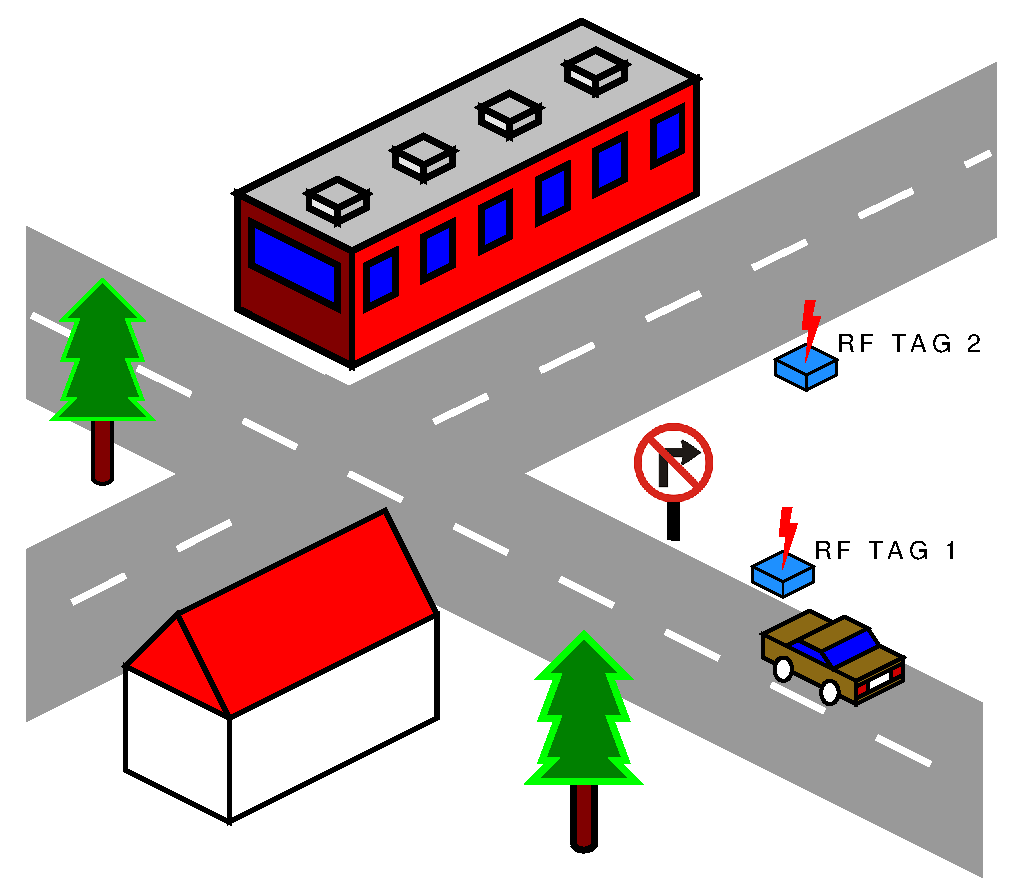
\includegraphics[width=60mm,height=50mm]{img/rfid2.eps}
\caption{Sample scenario for detecting directional regulation violations.}
\label{fig:dirreg}
\end{center}
\end{figure}

In the prolog implementation as shown in Figure \ref{fig:dir}, the rule definition for violation detection and examples for possible facts asserted by the sensor systems are given below. 

Please note that the probabilities are decreasing over time after the facts are asserted. Therefore, the probability of the violation may slightly differ from the multiplication of the probabilities of the facts.

\begin{mylisting}
Rules
\vspace*{2pt}\hrule
\begin{verbatim}
%rule declaration
violation(V,A,P) :- sign_detected(V),
                    rfid_detected(pre,V),
                    rfid_detected(post,V), 
                    gps_node_property(post,V), 
                    gps_node_property(pre,V), 
                    A is "N/A",
                    prob(P),
                    P>0.8.
\end{verbatim}

Query
\vspace*{2pt}\hrule
\begin{verbatim}

Exec: assert("0.9999::T::sign_detected(no_turn_left)").
Exec: assert("1::T::rfid_detected(pre,no_turn_left)").
Exec: assert("0.9110::T::gps_node_property(pre,no_turn_left)").
Exec: assert("0.8962::T::gps_node_property(post,no_turn_left)").
Exec: assert("1::T::rfid_detected(post,no_turn_left)").

Exec: violation(V,A,P).
Prob for this answer:0.816324396689487

P = 0.816324396689487
V = no_turn_left
A = "N/A"
\end{verbatim}
\end{list}\caption{Prolog program for directional regulation violations.}
\label{fig:dir}
\end{mylisting}

In the BN design, the network and the human expert provided probability values are given in Figure \ref{fig:bnsign}. The probability values may be assigned considering the possible false recognition of the signs. For example, the 'no U turn' sign can be detected as 'no left turn' sign by the vision module. If the human expert considers these possible conflicts while making the probability assessments, then the system has more chance of recovering its error by using the information provided by the other sensors.
\begin{figure}[ht]
\begin{center}
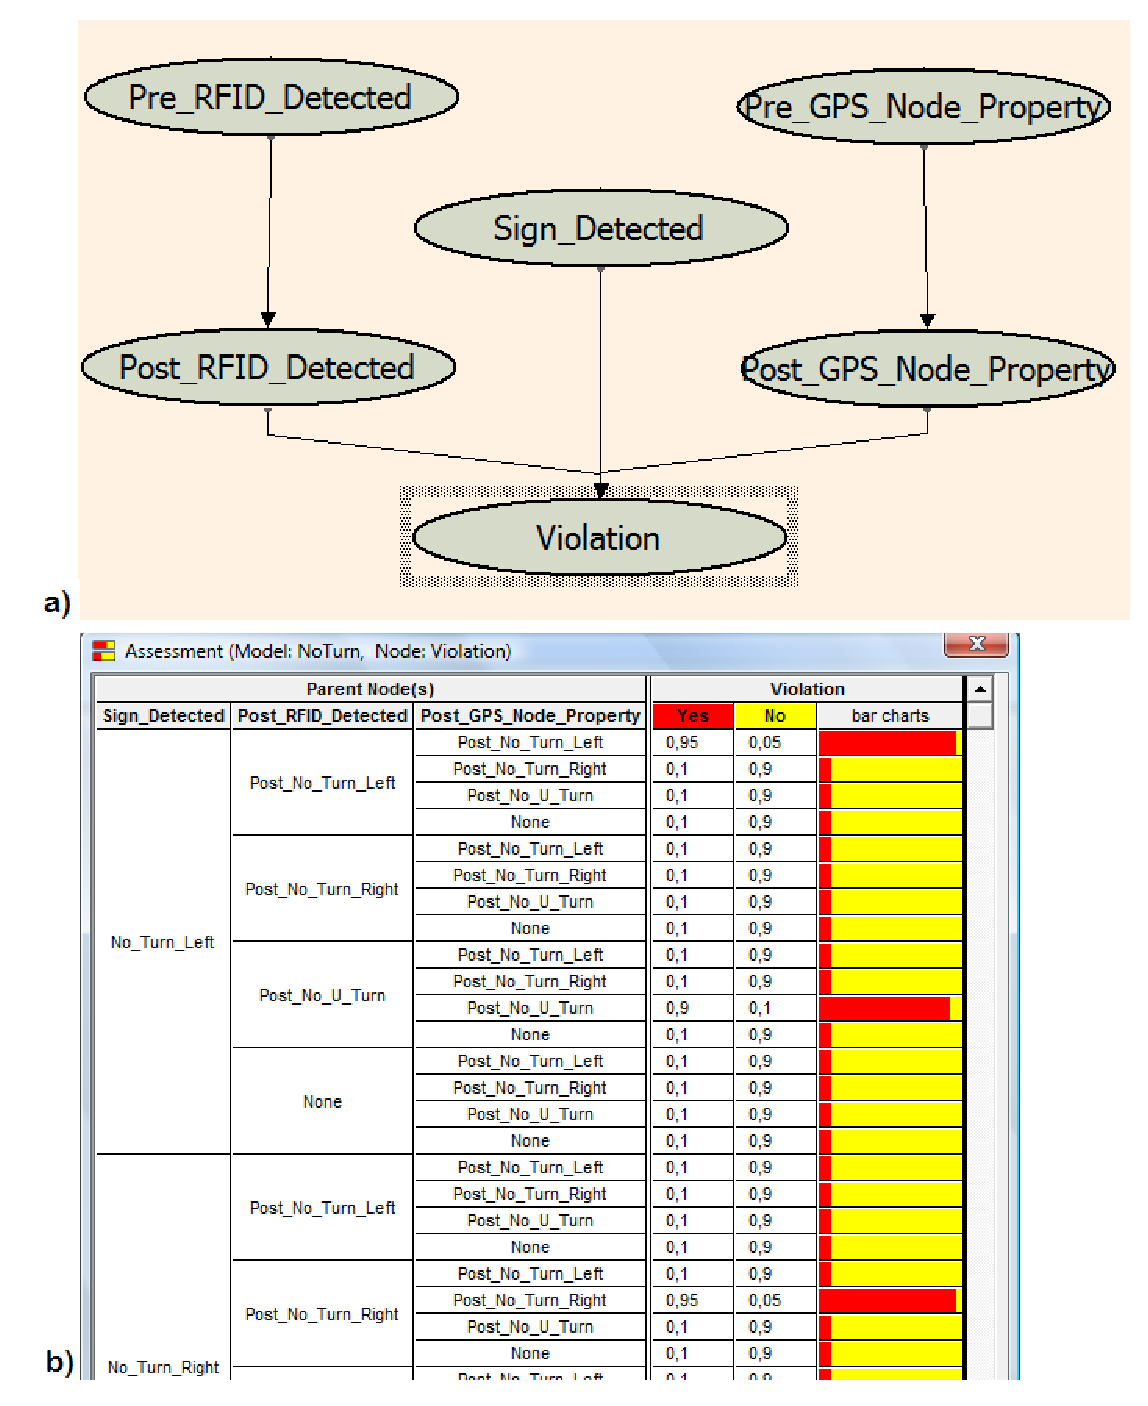
\includegraphics[scale=0.666]{img/no_turn_bn.eps}
\caption{Directional regulation's a) belief network and b) property assessments.}
\label{fig:bnsign}
\end{center}
\end{figure}

\subsubsection{Violation of Speed Limitation}

Speed limitations are usually indicated by red circular signs across Europe. These circular signs contain a number which is the maximum allowed speed limit for the motorway it is assigned for. GPS input can be used as well as visual and RF inputs for detecting the speed limit violations \cite{ogrady_garmin_2009}. In addition, the proposed method also uses information gathered from the vehicle itself. The speed of the vehicle is assumed to be supplied by the vehicle.

\begin{figure}[ht]
\begin{center}
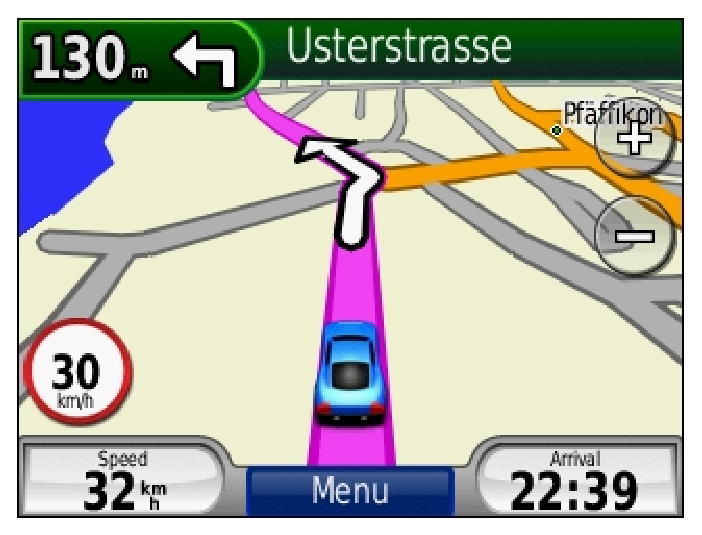
\includegraphics[width=44mm,height=33mm]{img/gpsspeed.eps}
\caption{Speed limit aware GPS application.}
\label{fig:gpsspeed}
\end{center}
\end{figure}

The prolog rules for speed limit violation detection are given in Figure \ref{fig:slv}.

\begin{mylisting}
Rules
\vspace*{2pt}\hrule
\begin{verbatim}
%rule declaration
violation(V,A,P) :- gps_node_property(V,L),
                    velocity_exceeds(S),
                    sign_detected(V,L),
                    S>=L,
                    atom_chars(S,L1), append(L1,[95],L2), 
                    atom_chars(L,L3), append(L2,L3,L4), atom_chars(A,L4),
                    prob(P),
                    P>0.9.
\end{verbatim}

Query
\vspace*{2pt}\hrule
\begin{verbatim}

Exec: assert("1.0000::T::sign_detected(speed_limit,30)").
Exec: assert("0.9759::T::gps_node_property(speed_limit,30)").
Exec: assert("1::T::velocity_exceeds(50)").

Exec: violation(V,A,P).
Prob for this answer:0.975898794128071

P = 0.975898794128071
V = speed_limit
A = '50_30'

\end{verbatim}
\end{list}\caption{Prolog program for speed limit violations.}
\label{fig:slv}
\end{mylisting}

Similarly, the BN implementation benefits from the vision, RF and GPS inputs. The probability assessments are again given by the human expert. The network diagram and assessments are shown in Figure \ref{fig:bnspeed}.

\begin{figure}[ht]
\begin{center}
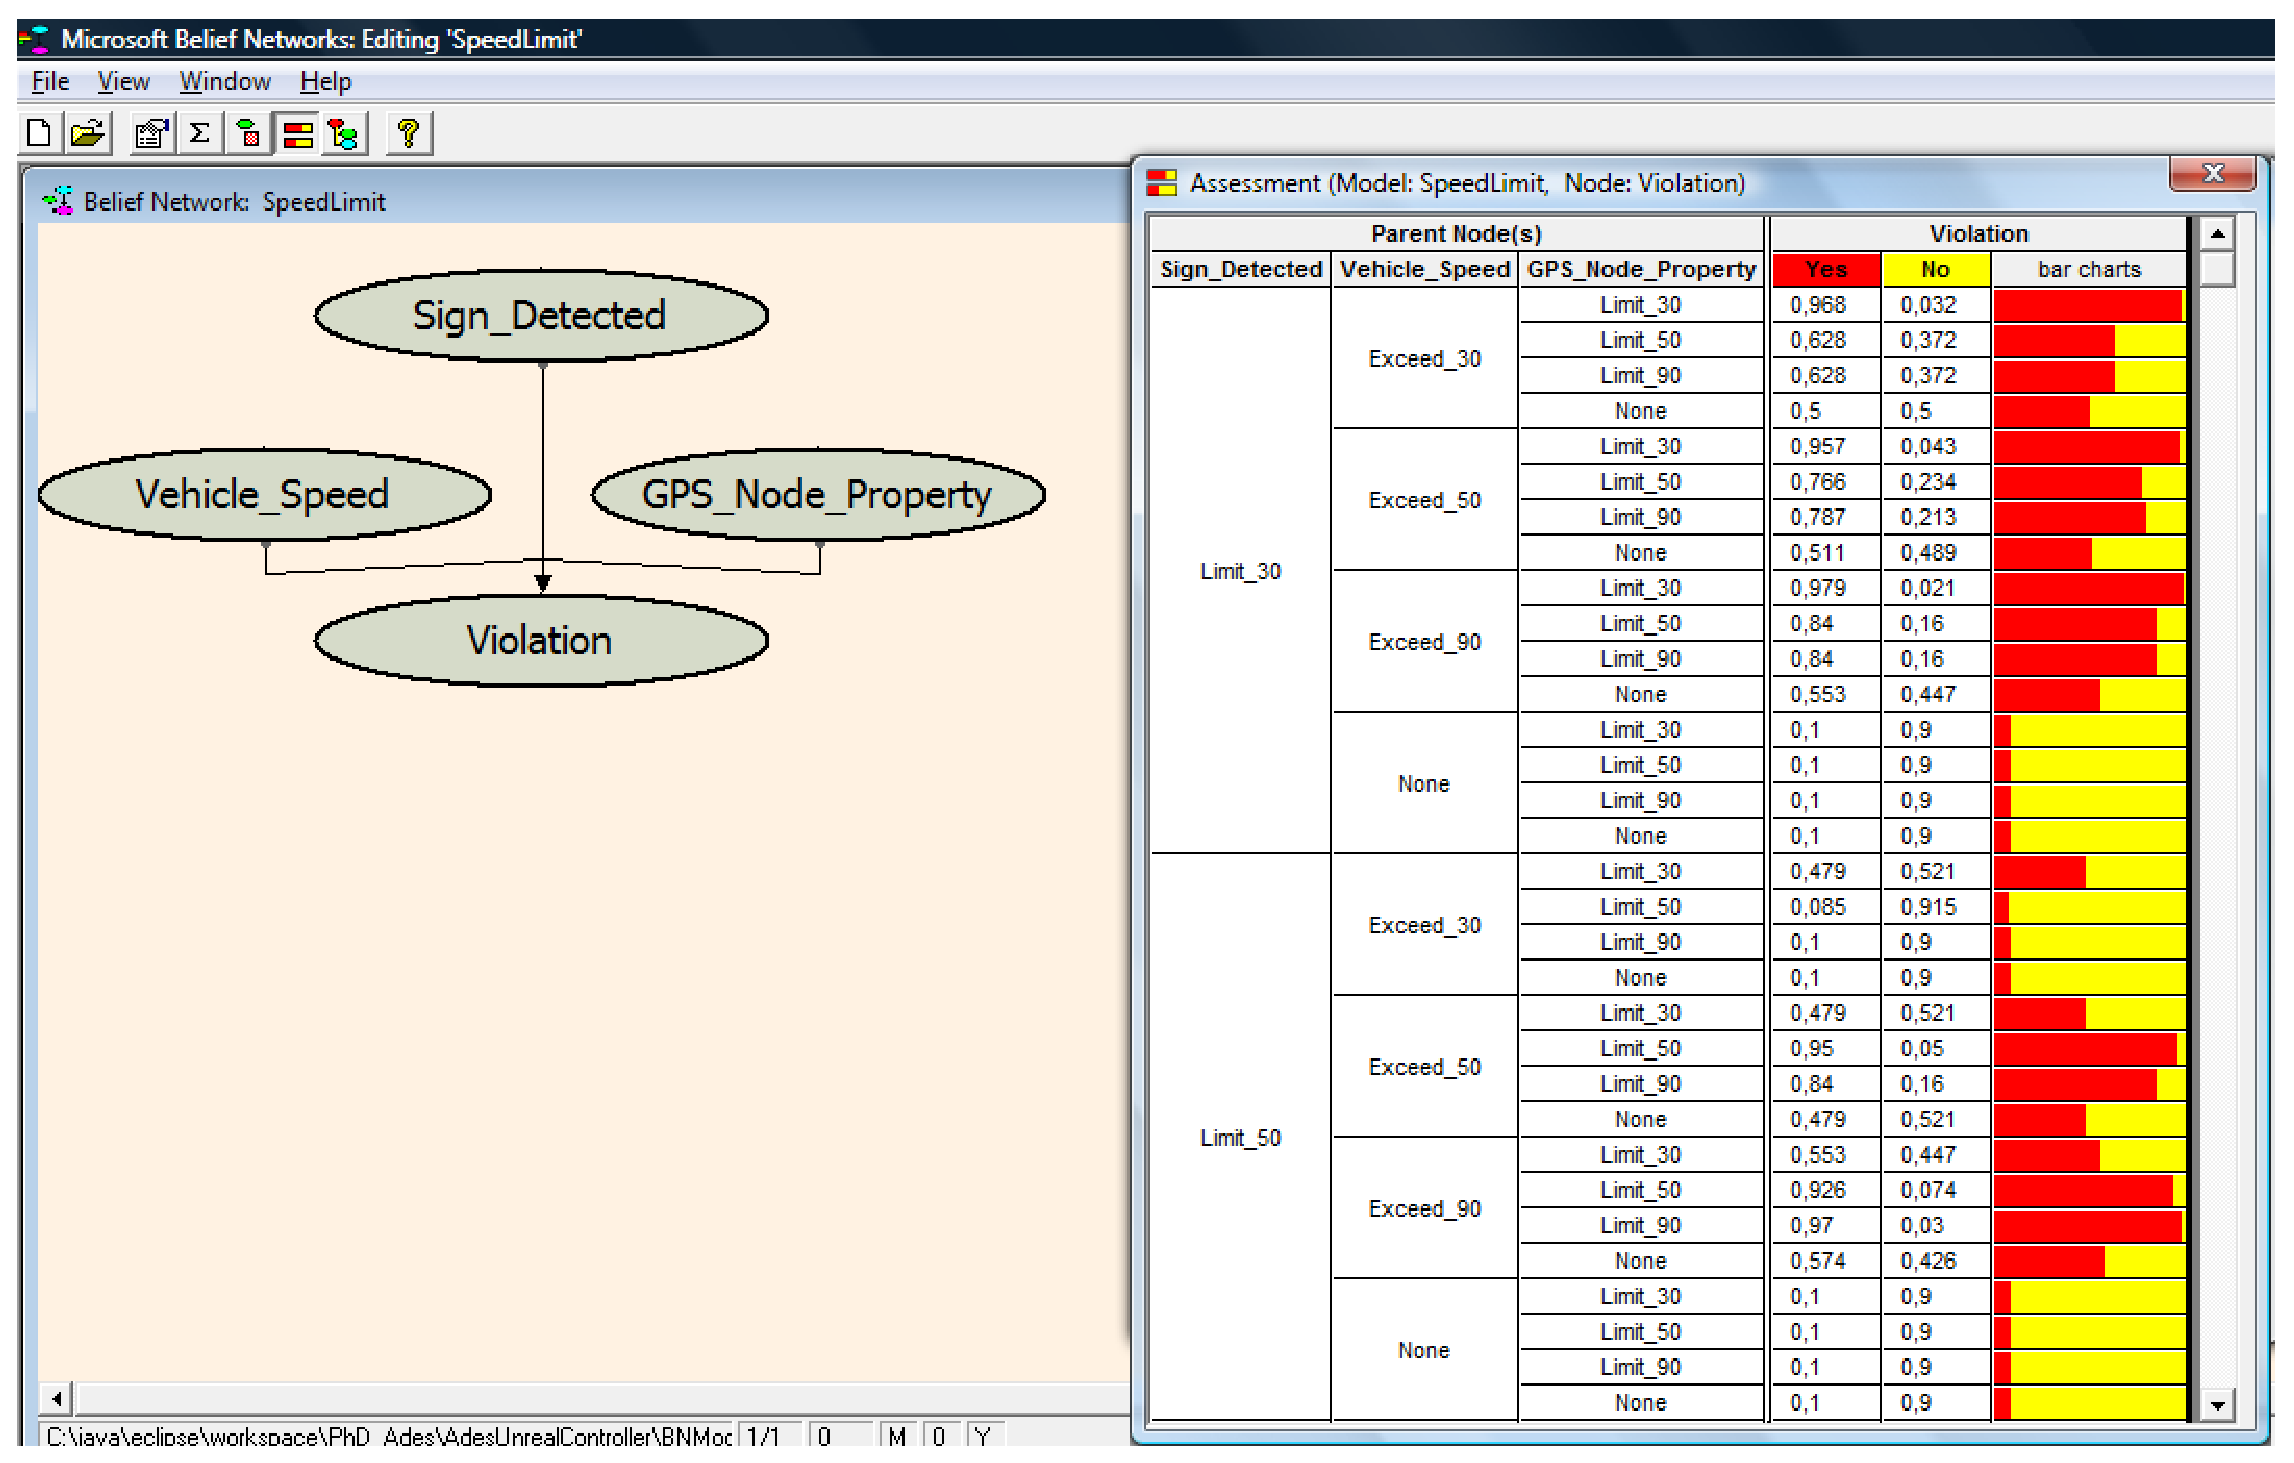
\includegraphics[width=150mm]{img/speed_bn.eps}
\caption{The belief network and it's property assessments for speed limitations.}
\label{fig:bnspeed}
\end{center}
\end{figure}

\subsubsection{Illegal Overtaking}

Illegal overtaking occurs during the course of passing a slower car under unsafe conditions. The overtake forbidden sign is given in Figure \ref{fig:otfb}

\begin{figure}[ht]
\begin{center}
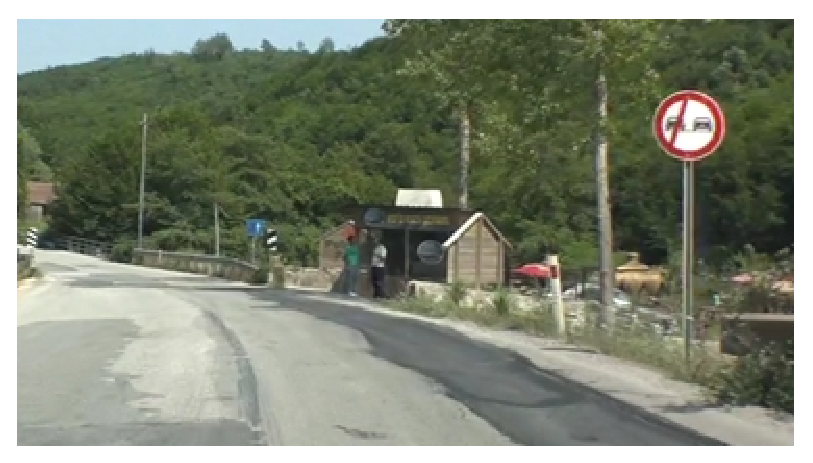
\includegraphics[width=64mm,height=36mm]{img/otfb.eps}
\caption{Overtake forbidden sign.}
\label{fig:otfb}
\end{center}
\end{figure}

The prolog rules for illegal overtaking detection are given in Figure \ref{fig:illeg}.

\begin{mylisting}
Rules
\vspace*{2pt}\hrule
\begin{verbatim}
%rule declaration
violation(V,A,P) :- sign_detected(no_overtake),
                    rfid_detected(no_overtake),
                    gps_node_property(no_overtake),
                    lane_departure(left),
                    A is "N/A",
                    V is "no_overtake",
                    prob(P).
\end{verbatim}
\end{list}\caption{Prolog program for illegal overtaking.}
\label{fig:illeg}
\end{mylisting}

The BN implementation of illegal overtaking is similar to speed limitation. However the probability assessment is relatively easy since the nodes has less attributes. The network and the probability assessment are given in Figure \ref{fig:bnillegal}.

\begin{figure}[ht]
\begin{center}
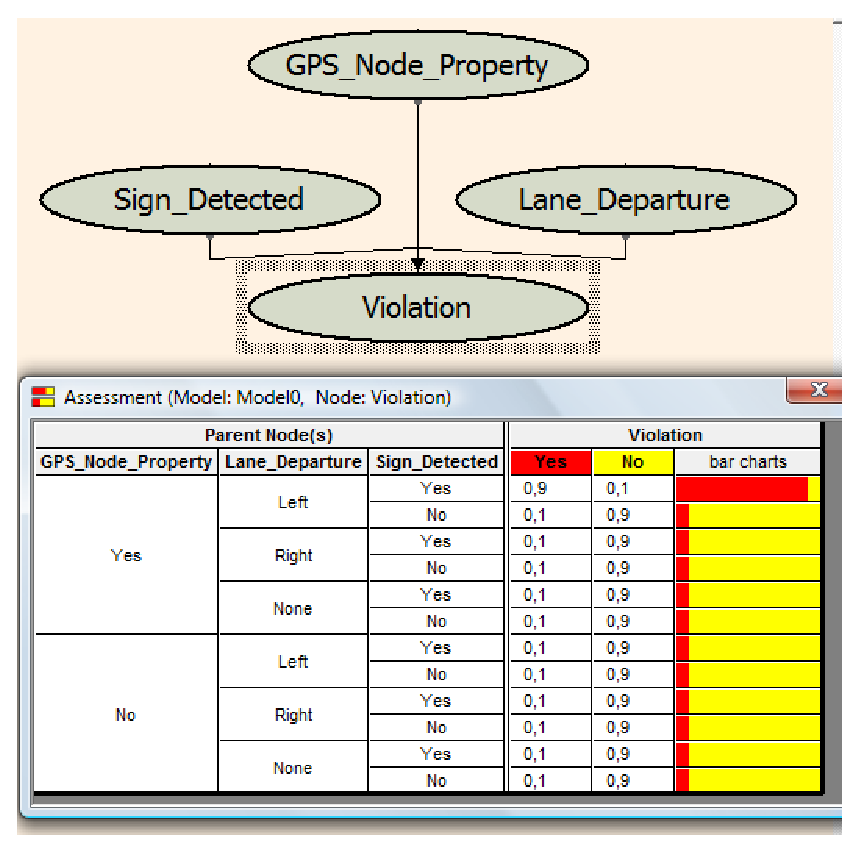
\includegraphics[width=100mm]{img/overtake_bn.eps}
\caption{The belief network and it's property assessments for illegal overtaking.}
\label{fig:bnillegal}
\end{center}
\end{figure}

\subsubsection{Violation of Red Traffic Lights}

The assertion of the red light rule is similar to directional regulations as shown in Figure \ref{fig:rfid3}.  However, red light rules are temporary. Which means that, the rule is strongly related with time. Since it is usually hard to recognize the traffic signs with the vision system, an RFID system with active tags can be used for this purpose. However, the RF system should contain active RF tags since the tags should be responding for a specific period of time. The system certainly can benefit from a visual feedback for the traffic lights. The traffic light detection can be used for enforcing the rules on crossroads like blocking the road in heavy traffic conditions.

\begin{figure}[ht]
\begin{center}
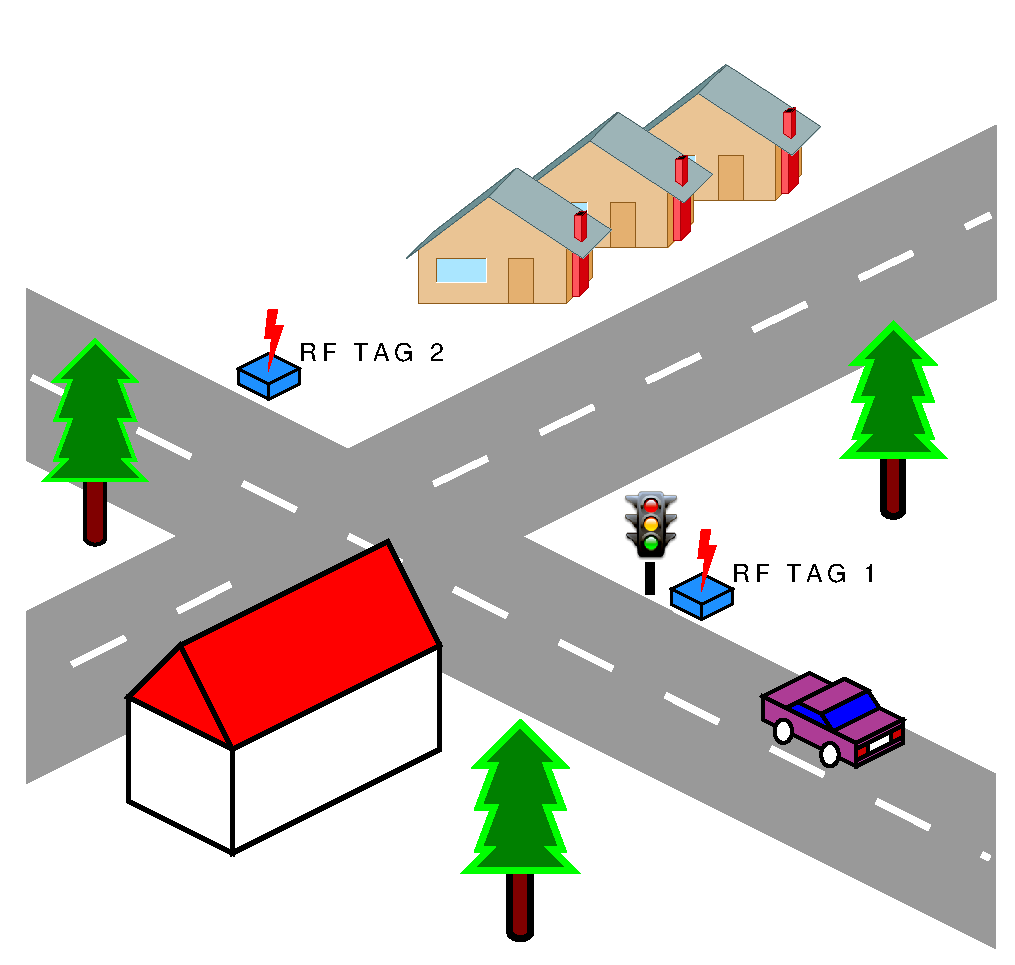
\includegraphics[width=60mm,height=50mm]{img/rfid3.eps}
\caption{Sample scenario for red light violations.}
\label{fig:rfid3}
\end{center}
\end{figure}

The prolog rules for red ligth violation detection are given in Figure \ref{fig:red}.

\begin{mylisting}
Rules
\vspace*{2pt}\hrule
\begin{verbatim}
%rule declaration
violation(V,A,P) :- rfid_detected(pre,light_red),
                    rfid_detected(post,light_red),
                    gps_node_property(traffic_lights),
                    A is "N/A",
                    V is "red_light",
                    prob(P).
\end{verbatim}
\end{list}\caption{Prolog program for red light violation.}
\label{fig:red}
\end{mylisting}

The BN implementation of traffic light regulations is similar to directional regulations. The vehicle should sense both pre and post RF tag to violate the traffic rule. The network and the probability assessment are given in Figure \ref{fig:bnredlight}.

\begin{figure}[ht]
\begin{center}
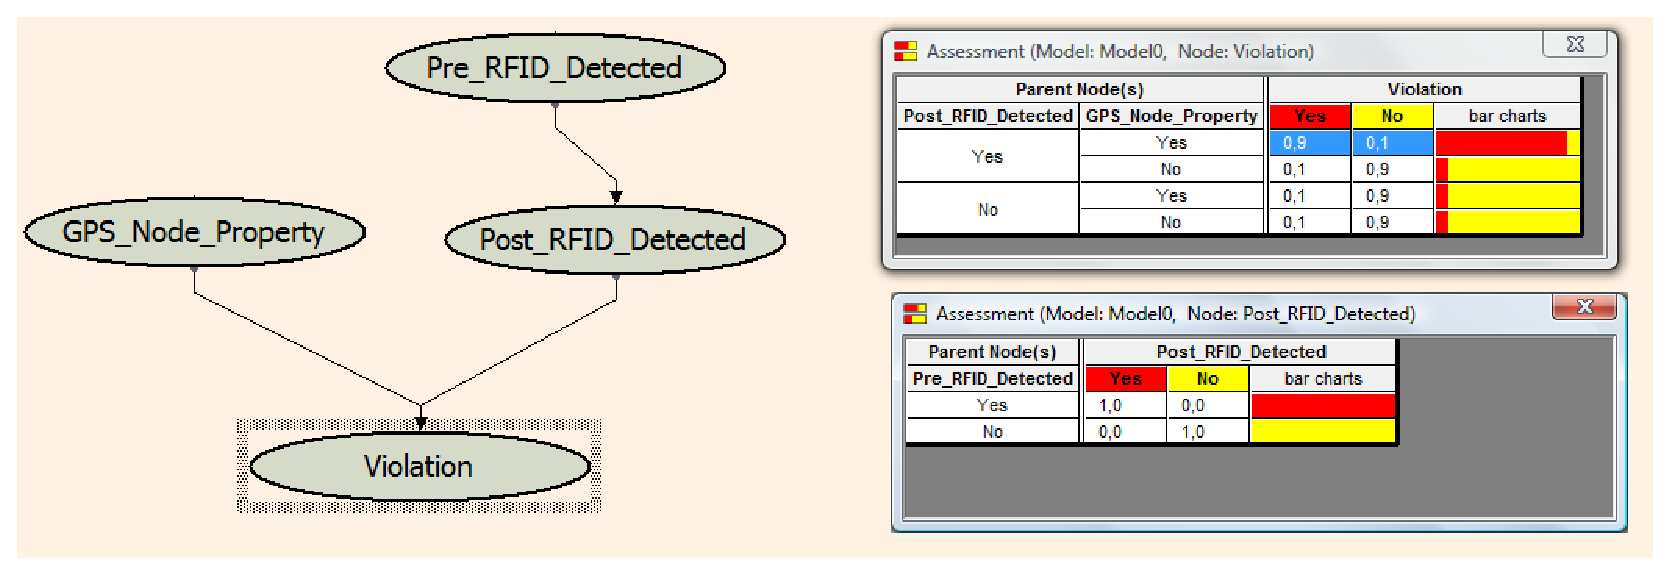
\includegraphics[width=140mm]{img/redlight_bn.eps}
\caption{The belief network and it's property assessments for traffic light regulations.}
\label{fig:bnredlight}
\end{center}
\end{figure}


\section{Modeling Driver Aggressiveness}

There are various social studies about the causes of driver aggressiveness \cite{lajunen_does_1999} or results of this aggression \cite{shinar_aggressive_1998}. According to the Florida Department of Highway Safety and Motor Vehicles' Aggressive Driver Study \cite{florida_aggresive_1999}, there is no well defined definition of the term \textit{aggressive driving}. A driver who performs actions such as weaving in and out of traffic lanes to get ahead, or tailgating can be defined as an aggressive driver. Exceeding speed limits, changing lanes frequently, and cutting other drivers way ahead are common behaviors of aggressive drivers. The aggressive drivers exhibit more hard deceleration, acceleration, and swerve maneuvers during baseline driving than did the safe drivers, which may increase drivers' relative crash risk above that of normal driving \cite{klauer_comparing_2008}.

In the ADES project, driver aggressiveness is measured using the number of traffic violations performed by the driver. Each violation increases the coefficient $c$ by one. If the driver does not violate any rules for a specific period of time, this coefficient is decreased by one. This coefficient is used as the multiplicand of the threshold value used against the violation probabilities of the expert systems as shown in Equation \ref{eq12}.
\begin{eqnarray}
\label{eq12}
Violation &=& \left\{\begin{array}{l} Yes \rightarrow p>t\times(1-\alpha{\times}c/c_{max}), 0<\alpha<1 \\ No \rightarrow o/w \end{array}\right.
\end{eqnarray}
The $c_{max}$ value is the maximum possible aggressiveness coefficient for any driver. $p$ is the output of the expert system and $t$ is the predefined threshold value for accepting the probability of the expert system output as violation. Finally, $\alpha$ is the strength of the effect of the driver aggression model on the threshold. Its value is set to $0.1$ in the current implementation which means the maximum effect of the driver aggression model can be $0.1$ on the threshold value.

\chapter{APPLICATIONS}
\label{chapapp}
Two main applications have been developed for the ADES project. The first one, the ADES detector, is used for detecting road lanes and traffic signs. The second application is a simulation environment which is used as a test bed for both sensor modules and the inference engine. 

\section{The ADES Detector}
\label{adesdetector}
The ADES detector application is designed for processing video feedbacks for detecting road lanes and recognizing traffic signs. This video feedback can be a real-time streaming video feed from a camera, a recorded video stream, a stream fed from network or any memory mapped image source. The main purpose of this tool is to test the performances of the vision processors. The results of different processors can be visualized in real-time as shown in Figure \ref{fig:adesdetector}. The red lines on the figure are the detected road lanes where the rightmost images are the recognized circular traffic sign and the detected triangular sign.
\begin{figure}[ht]
\begin{center}
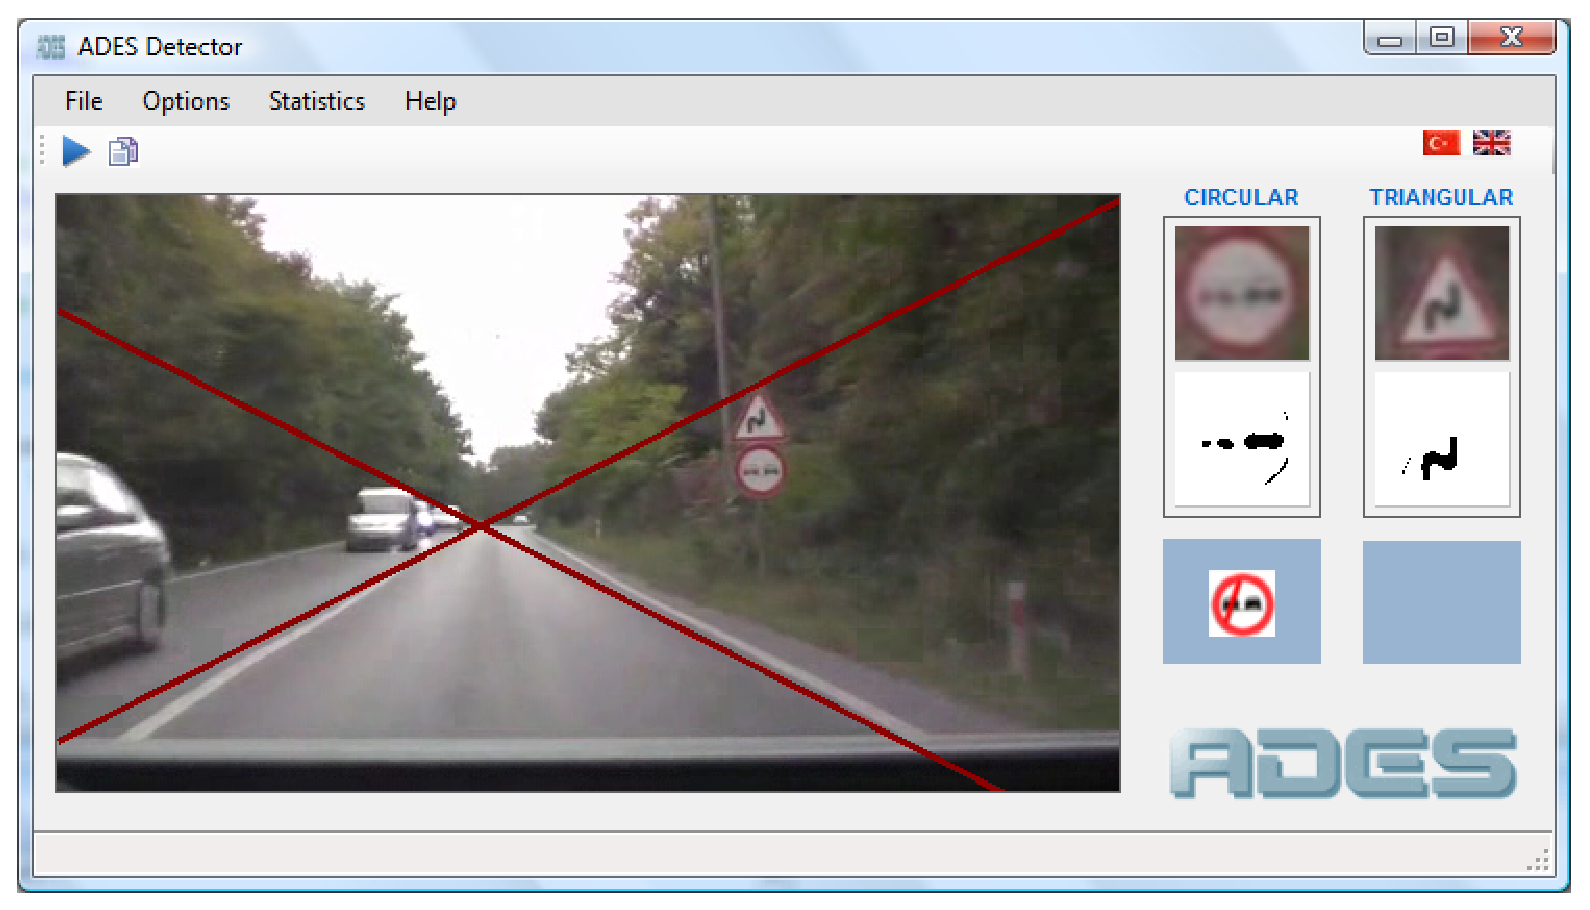
\includegraphics[width=120mm]{img/ADESDetector.eps}
\caption{The ADES Detector.}
\label{fig:adesdetector}
\end{center}
\end{figure}
Another very important service of the ADES detector application is the training of the neural networks and support vector machines used for sign identification. The user can initiate the training sequence after appropriately placing the training files to the corresponding file folders. The NN training phase creates a network for each sign. The SVM training phase creates a single model for all signs.

The application also provides an option for using the Linear Discriminant Analysis (LDA) features instead of all input vector for traffic signs \cite{bochkanov_alglib_2008,mika_fisher_1999}. The LDA process traverses all training files and figures out the most important parametric number of pixels on the traffic sign images. Then the training can be done by using these features, and similarly the test process can also use these features.

\section{ADES Simulation Environment}
Although the ADES project targets the real physical environment, the development process can be accelerated by the use of a realistic simulation environment. Our choice for the simulation engine is the \textit{Unreal Engine} which provides the physics engine and the renderer. The success of this engine makes it a favorite tool for both robotic researchers and game developers. 

The interaction between the Unreal Engine, USARSim and the Unreal ADES controller is shown in Figure \ref{fig:unrealades}. The system has three components, each of which can be run on separate computers. The first part is the Unreal Engine with the USARSim expansion. This is the core of the simulation system where rendering and physics calculations are performed. The second part is the extended version of the USARSim Image Server (UPIS). The role of this part is serving vision information to the custom applications rather than the Unreal Engine's default client application. The last part, which is the ADES Unreal Controller, is a client for the USARSim and the UPIS servers. The details of each module are given in the following sections.

\begin{figure}[ht]
\begin{center}
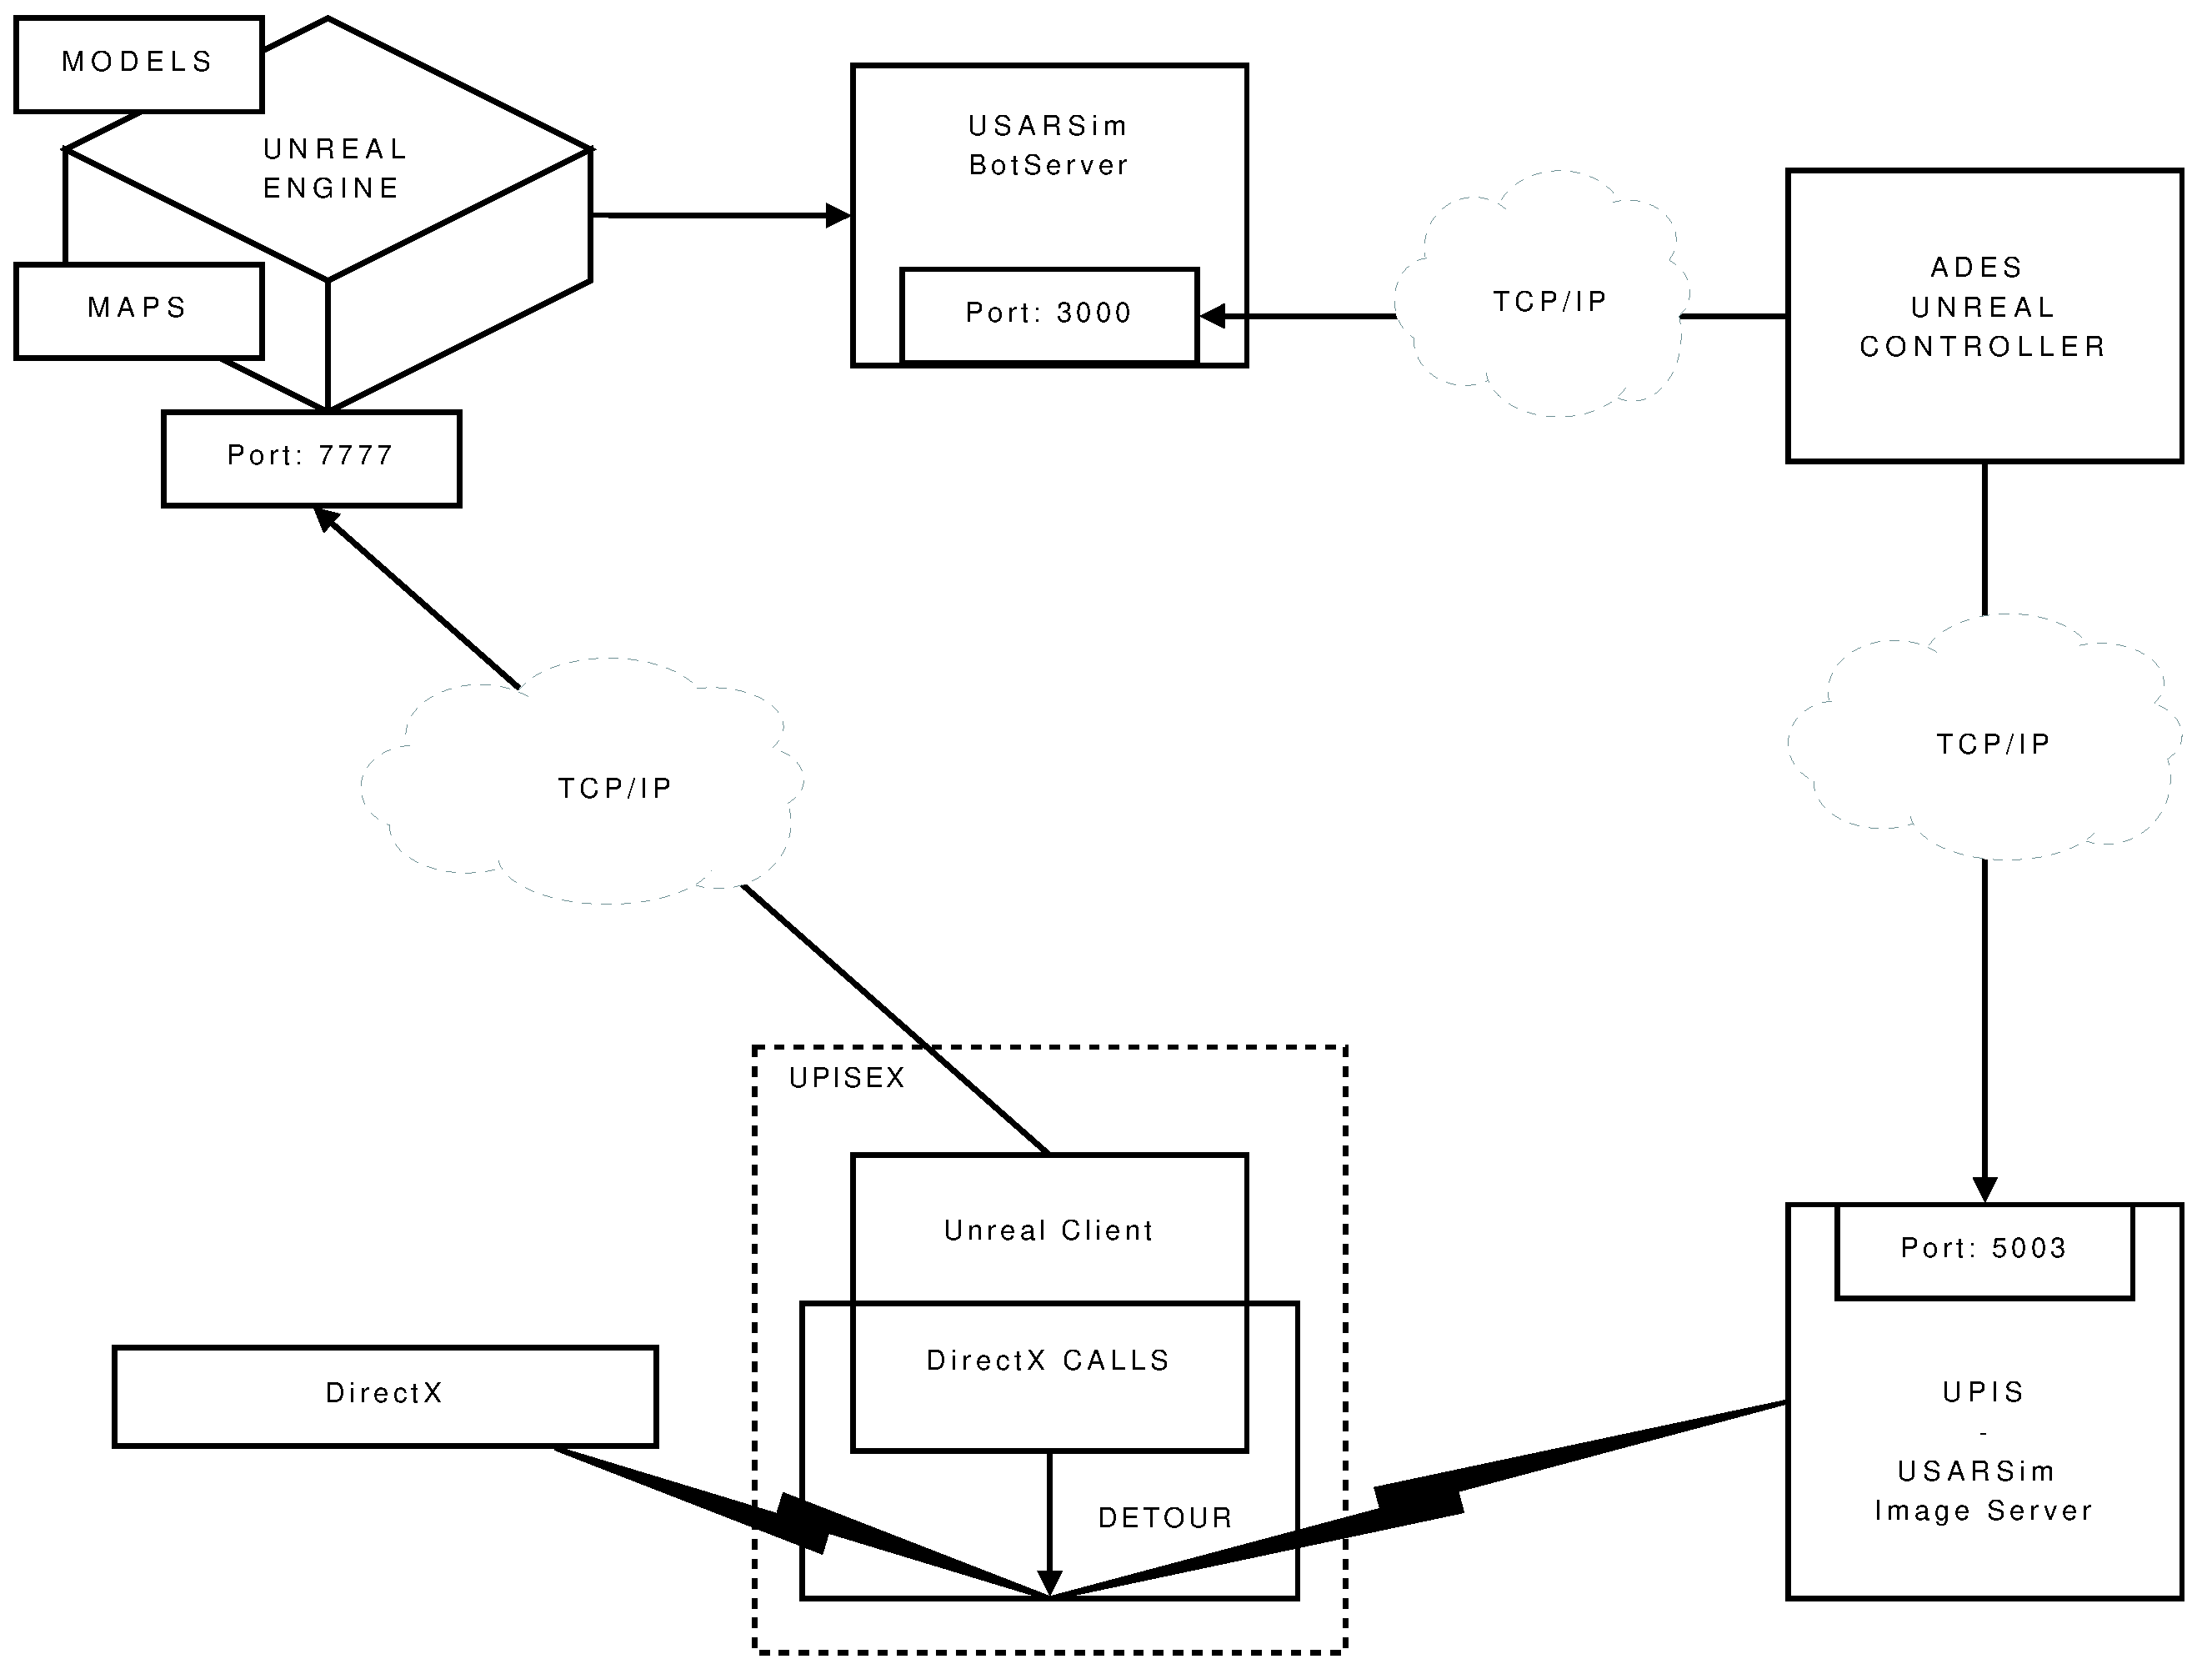
\includegraphics[width=100mm,height=90mm]{img/unrealades.eps}
\caption{Interaction between Unreal Engine, USARSim and Unreal ADES controller.}
\label{fig:unrealades}
\end{center}
\end{figure}

\subsection{Unreal Engine}
The Unreal Engine is a commercial game engine developed by Epic Games. Its first version, UE1, was announced in 1998. In 2002, the next version, UE2, was released. The ADES simulation environment is based on UE2.5, which is an improved version of UE2 and released a few years later. However, the latest version of the engine is UE3 and equipped with many advanced techniques. However the hardware requirements for this engine are not compatible with our project. Unfortunately, the UE2.5 engine is not freeware and can be obtained by purchasing the Unreal Tournament 2004 game. It also includes the physics engine, which is known as the Karma engine \cite{epic_karma_2002}.

Unreal Engine also provides an object oriented programming called the UnrealScript which is a high level programming environment for game developers. The Java style coding with built in basic tasks like object's event handling, automatic garbage collection, and many base classes for different kinds of actors enables fast and neat game development.

\subsection{USARSim}

USARSim is an Unreal Engine expansion for urban search and rescue (USAR) robots and environments. It is an open source research tool for the study of various kinds of robotic applications. USARSim platform can be used in many domains like Defense Advanced Research Projects Agency (DARPA) Urban Challenge or National Institute of Standards (NIST) Reference Test Facility for Autonomous Mobile Robots for Urban Search and Rescue. However, RoboCup Rescue Virtual Robots Championship is maybe the most important domain for us where the USARSim platform is used. The know-how gained from this project can also be transferred to the teams of our researchers in our laboratory who are planning to participate in this competition.

The USARSim environment provides numerous models for the use of researchers. We are using the Sedan class as our vehicle in the simulated environment. The object hierarchy and brief descriptions of these classes are given in Table \ref{tab:Sedan}.

\begin{table}[ht]
\vskip\baselineskip
\caption{The class hierarchy of Sedan class.}
~\vskip -1mm
\centering
{\scriptsize
\begin{tabular}{|r|r|r|}
\hline
           & \multicolumn{ 2}{|l|}{{\bf Unreal Classes (Commercial)}} \\
\hline
           & {\bf Class} & {\bf Description} \\
\hline
         1 &      Actor & The base class of every object that have a position in the Unreal world. \\
\hline
         2 &       Pawn & Parent class for all controlled entities. \\
\hline
         3 &    Vehicle & Parent class for all vehicles controlled by the player. \\
\hline
         4 &   KVehicle & Vehicles Karma physics. \\
\hline
           & \multicolumn{ 2}{|l|}{{\bf USARSim Classes (Open Source)}} \\
\hline
           & {\bf Class} & {\bf Description} \\
\hline
         5 &     KRobot & USARSim's physical robot base \\
\hline
         6 & GroundVehicle & Vehicles with wheels and steering \\
\hline
         7 & AckermanSteeredRobot & Ackerman Steered Vehicles \\
\hline
         8 &      Sedan & The Sedan class used by ADES Unreal Controller \\
\hline
\end{tabular}
}
\label{tab:Sedan}
\end{table}
In addition to various vehicle classes, USARSim also provides numerous sensors to equip these vehicles. In the current implementation of ADES simulation, the camera and the RF reader sensors are mounted on the Sedan as shown in Figure \ref{fig:Sedan}. In order to mount a sensor to the vehicle, it is sufficient to append the descriptive line to the definition of the vehicle in the Usarsim.ini file located at the System directory of the Unreal Engine. The current definition of the Sedan class is given in Figure \ref{fig:sedanconf}.
\begin{figure}[ht]
\begin{center}
\includegraphics[width=100mm,height=80mm]{img/Sedan.eps}
\caption{The Sedan in the ADES Unreal world.}
\label{fig:Sedan}
\end{center}
\end{figure}

\begin{mylisting}
From the Usarsim.ini file in UT2004$\backslash$System directory. 
\vspace*{2pt}\hrule
{\scriptsize
\begin{verbatim}
[USARBot.Sedan]
bDebug=False
Weight=5
Payload=2
ChassisMass=10
MaxTorque=200.0
MotorTorque=200.0
bMountByUU=False
JointParts=(PartName="RightFWheel",PartClass=class'USARModels.SedanTireRight' ...
JointParts=(PartName="LeftFWheel",PartClass=class'USARModels.SedanTireLeft',. ..
JointParts=(PartName="RightRWheel",PartClass=class'USARModels.SedanTireRight', ...
JointParts=(PartName="LeftRWheel",PartClass=class'USARModels.SedanTireLeft', ...
MisPkgs=(PkgName="CameraPanTilt",PkgClass=Class'USARMisPkg.CameraPanTilt')...
Cameras=(ItemClass=class'USARBot.RobotCamera',...
Sensors=(ItemClass=class'USARBot.GroundTruth', ...
Sensors=(ItemClass=class'USARBot.RFIDSensor', ...
Sensors=(ItemClass=class'USARBot.GPSSensor', ...
\end{verbatim}
}
\end{list}\caption{The definition of Sedan class.}
\label{fig:sedanconf}
\end{mylisting}

In this definition, there are several parameters about the physical properties of the vehicle. In addition, the tires of the vehicle also represented since the Sedan class is extended from AckermanSteeredRobot class. MisPkgs are used for defining objects which can accept Mission Packages. For example, the pan and tilt of a camera can be controlled by using Mission Packages. In the ADES project, since all of the sensors on the vehicle are fixed, Mission Packages are not used. The sensors on the Sedan are RF reader, Camera and GroundTruth. The GroundTruth sensor provides information about the position and orientation of the vehicle. Since this sensor is prone to cumulative errors, it is not used in the current implementation. However, the GPS sensor, which is also available in USARSim, will be used in near future.

USARSim also provides the USARDeathMatch game type which enables the BotServer. The BotServer opens a communication channel between the Unreal Engine and the outside world. Custom objects derived from the \textit{pawn} class can be initiated from remote controlling applications by connecting to this server. USARSim also provides its own communication protocol. The details of this protocol can be found on the USARSim manual \cite{carpin_usarsim:_2007}.

The USARSim games require maps to run on. Therefore, we developed an initial version of the ADES Unreal world by using the Unreal level editor.

\subsection{UnrealEd: Level Editor}

The ADES simulated environment is developed using the UnrealEd, which is the level editor of Unreal Engine. UnrealEd user interface is based on quad viewports which are side, front, top views and an additional perspective view as shown in Figure \ref{fig:UnrealEdQuad}.

\begin{figure}[ht]
\begin{center}
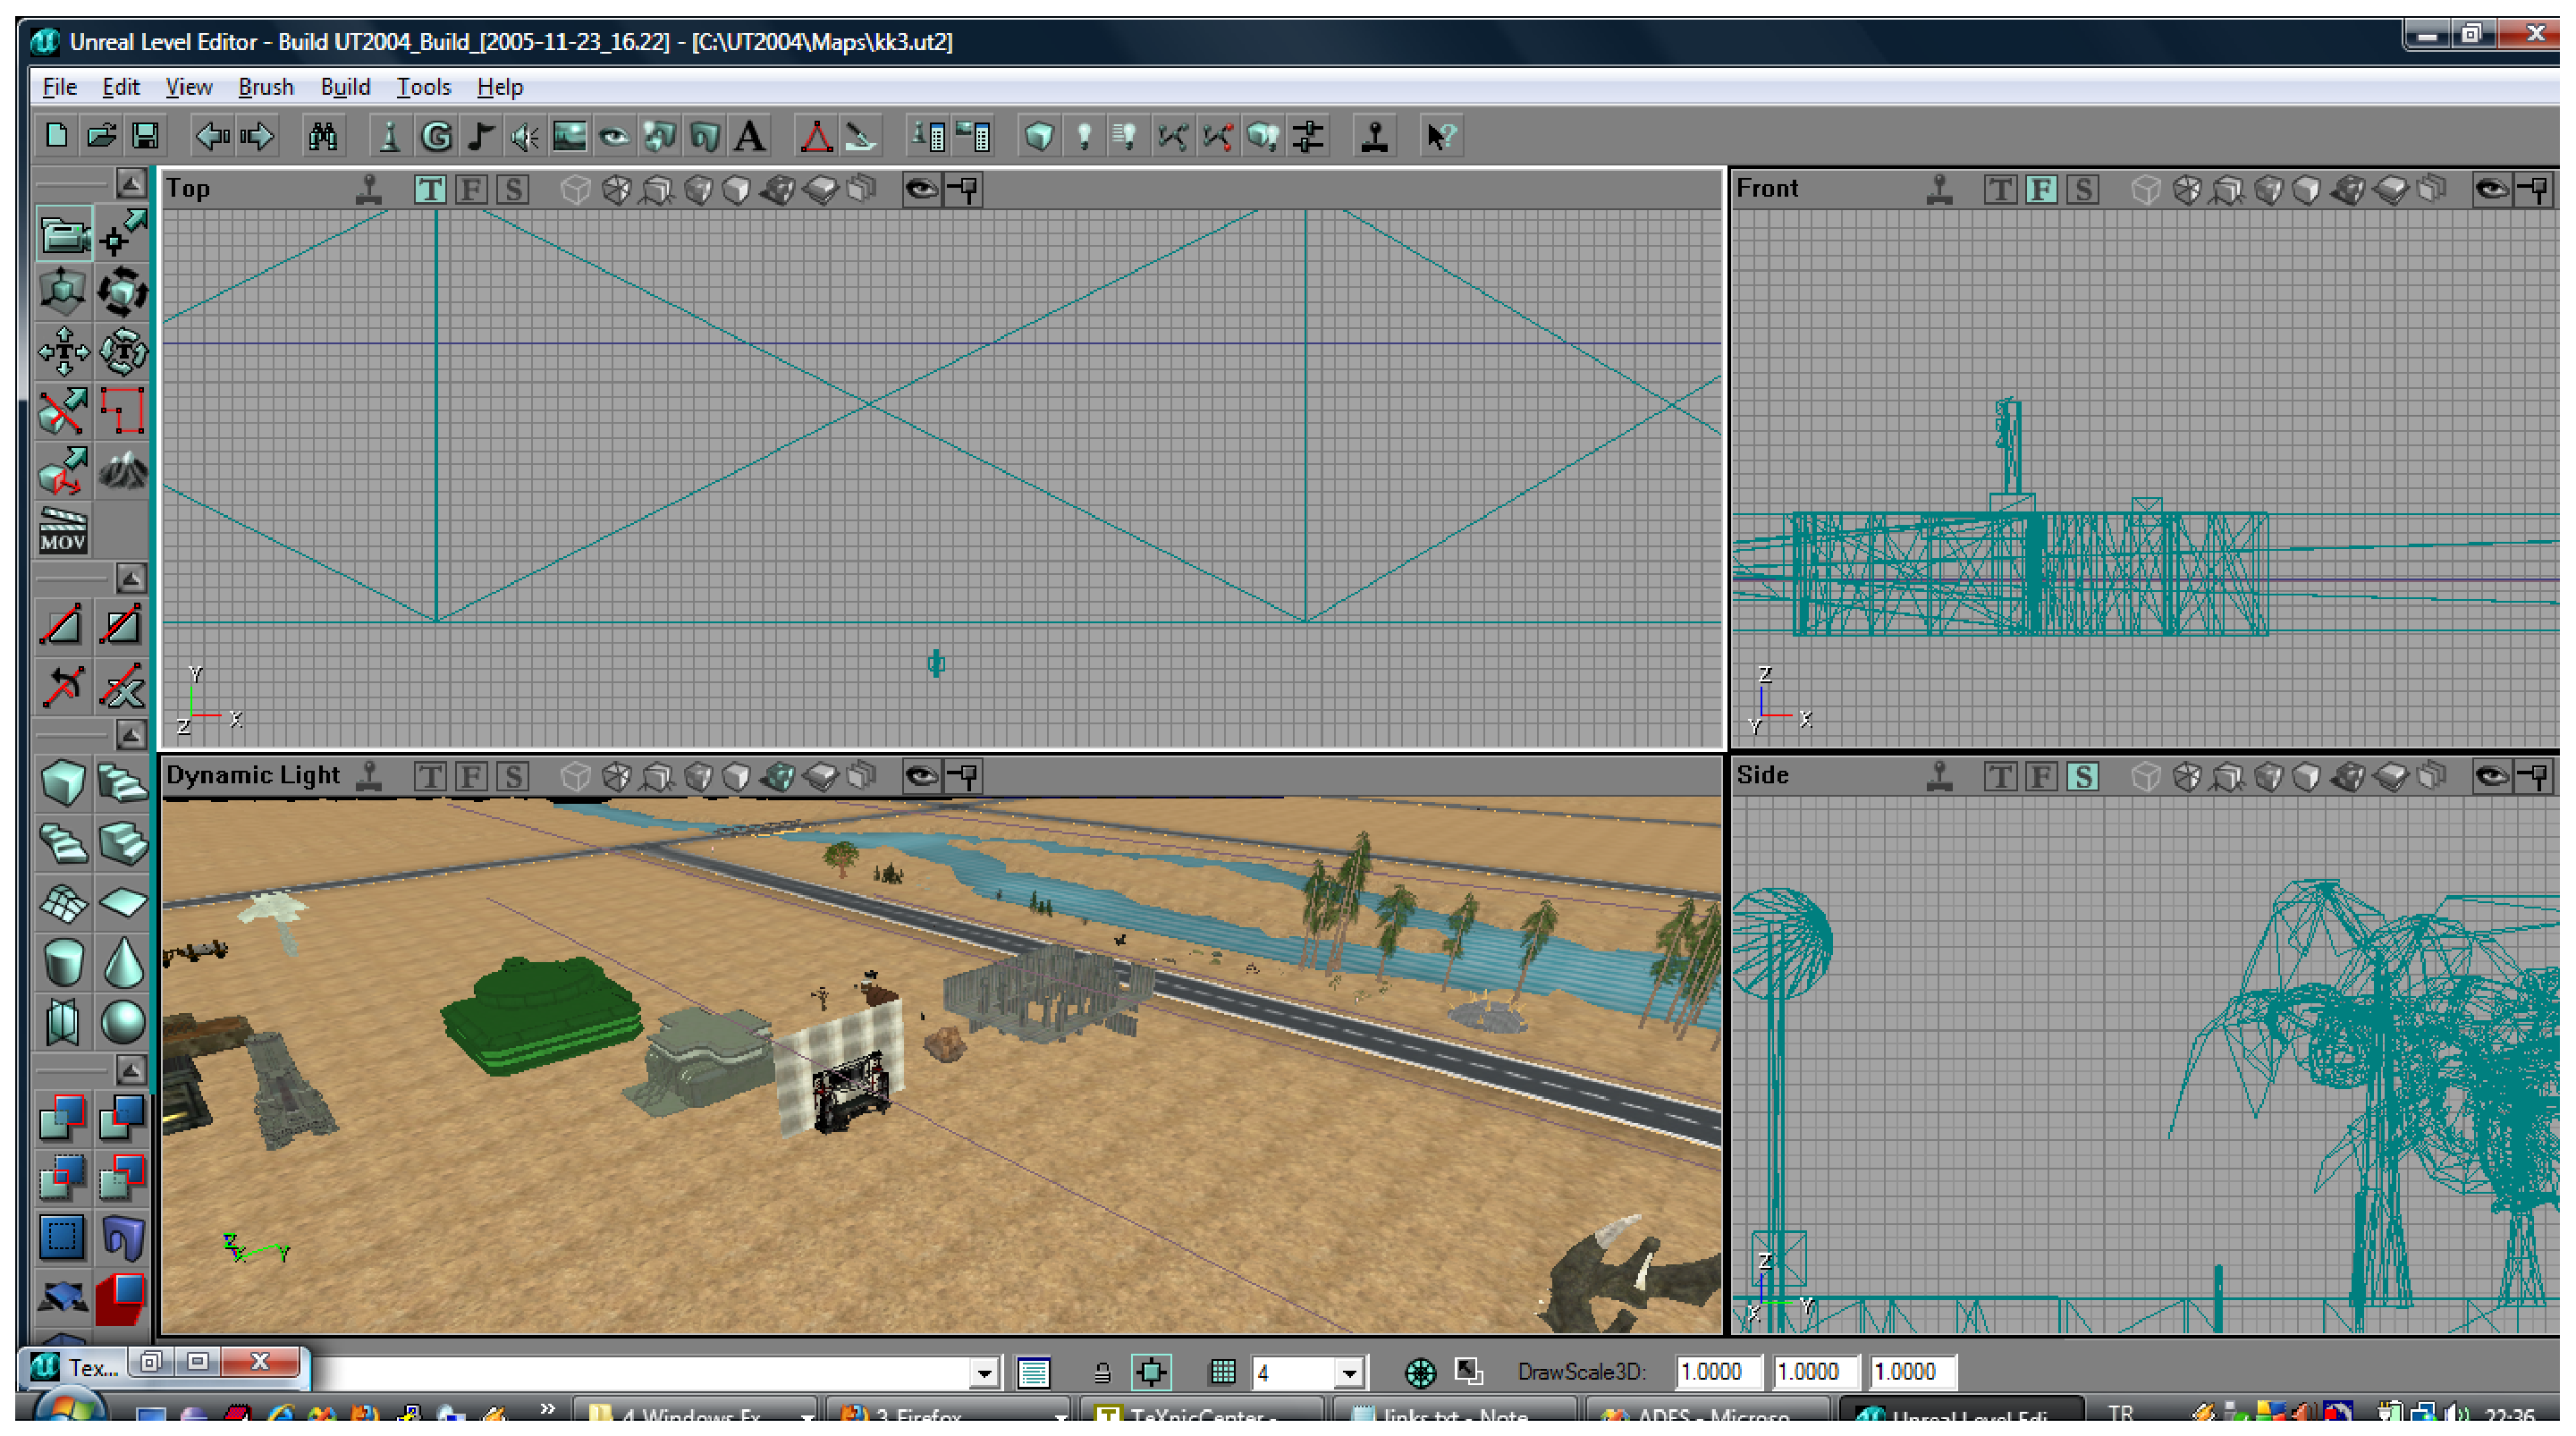
\includegraphics[width=150mm,height=90mm]{img/UnrealEdQuad.eps}
\caption{The ADES Unreal world in UnrealEd.}
\label{fig:UnrealEdQuad}
\end{center}
\end{figure}

The UnrealEd has subtractive and additive brushes for adding or removing objects with various shapes. Although the latest version of the UnrealEd supports both empty and filled initial spaces, we are using the former version which only supports filled initial spaces. Therefore, the initial step for creating an environment is carving a quite big rectangular object from the space.

The unreal editor has the following set of artifacts;
\begin{itemize}
    \item Actors: Any object that can be placed into the environment. These objects can be controlled pawns like Sedan, or, other items like pickups, decorations, zone information etc.
    \item Textures: Textures are images which can be applied to the new created shapes by using brushes.
    \item Static Meshes: The reusable objects which contain previously created shapes covered with textures.
    \item Meshes and Animations: Set of meshes which forms repeating animations for shapes.
    \item Other Artifacts: Sounds, Music, Prefabs (saved brushes).
\end{itemize}

In the ADES project different textures and static meshes are used. Some examples are given in Figure \ref{fig:StaticMesh}. Different actors are also placed for different purposes. 

\begin{figure}[ht]
\begin{center}
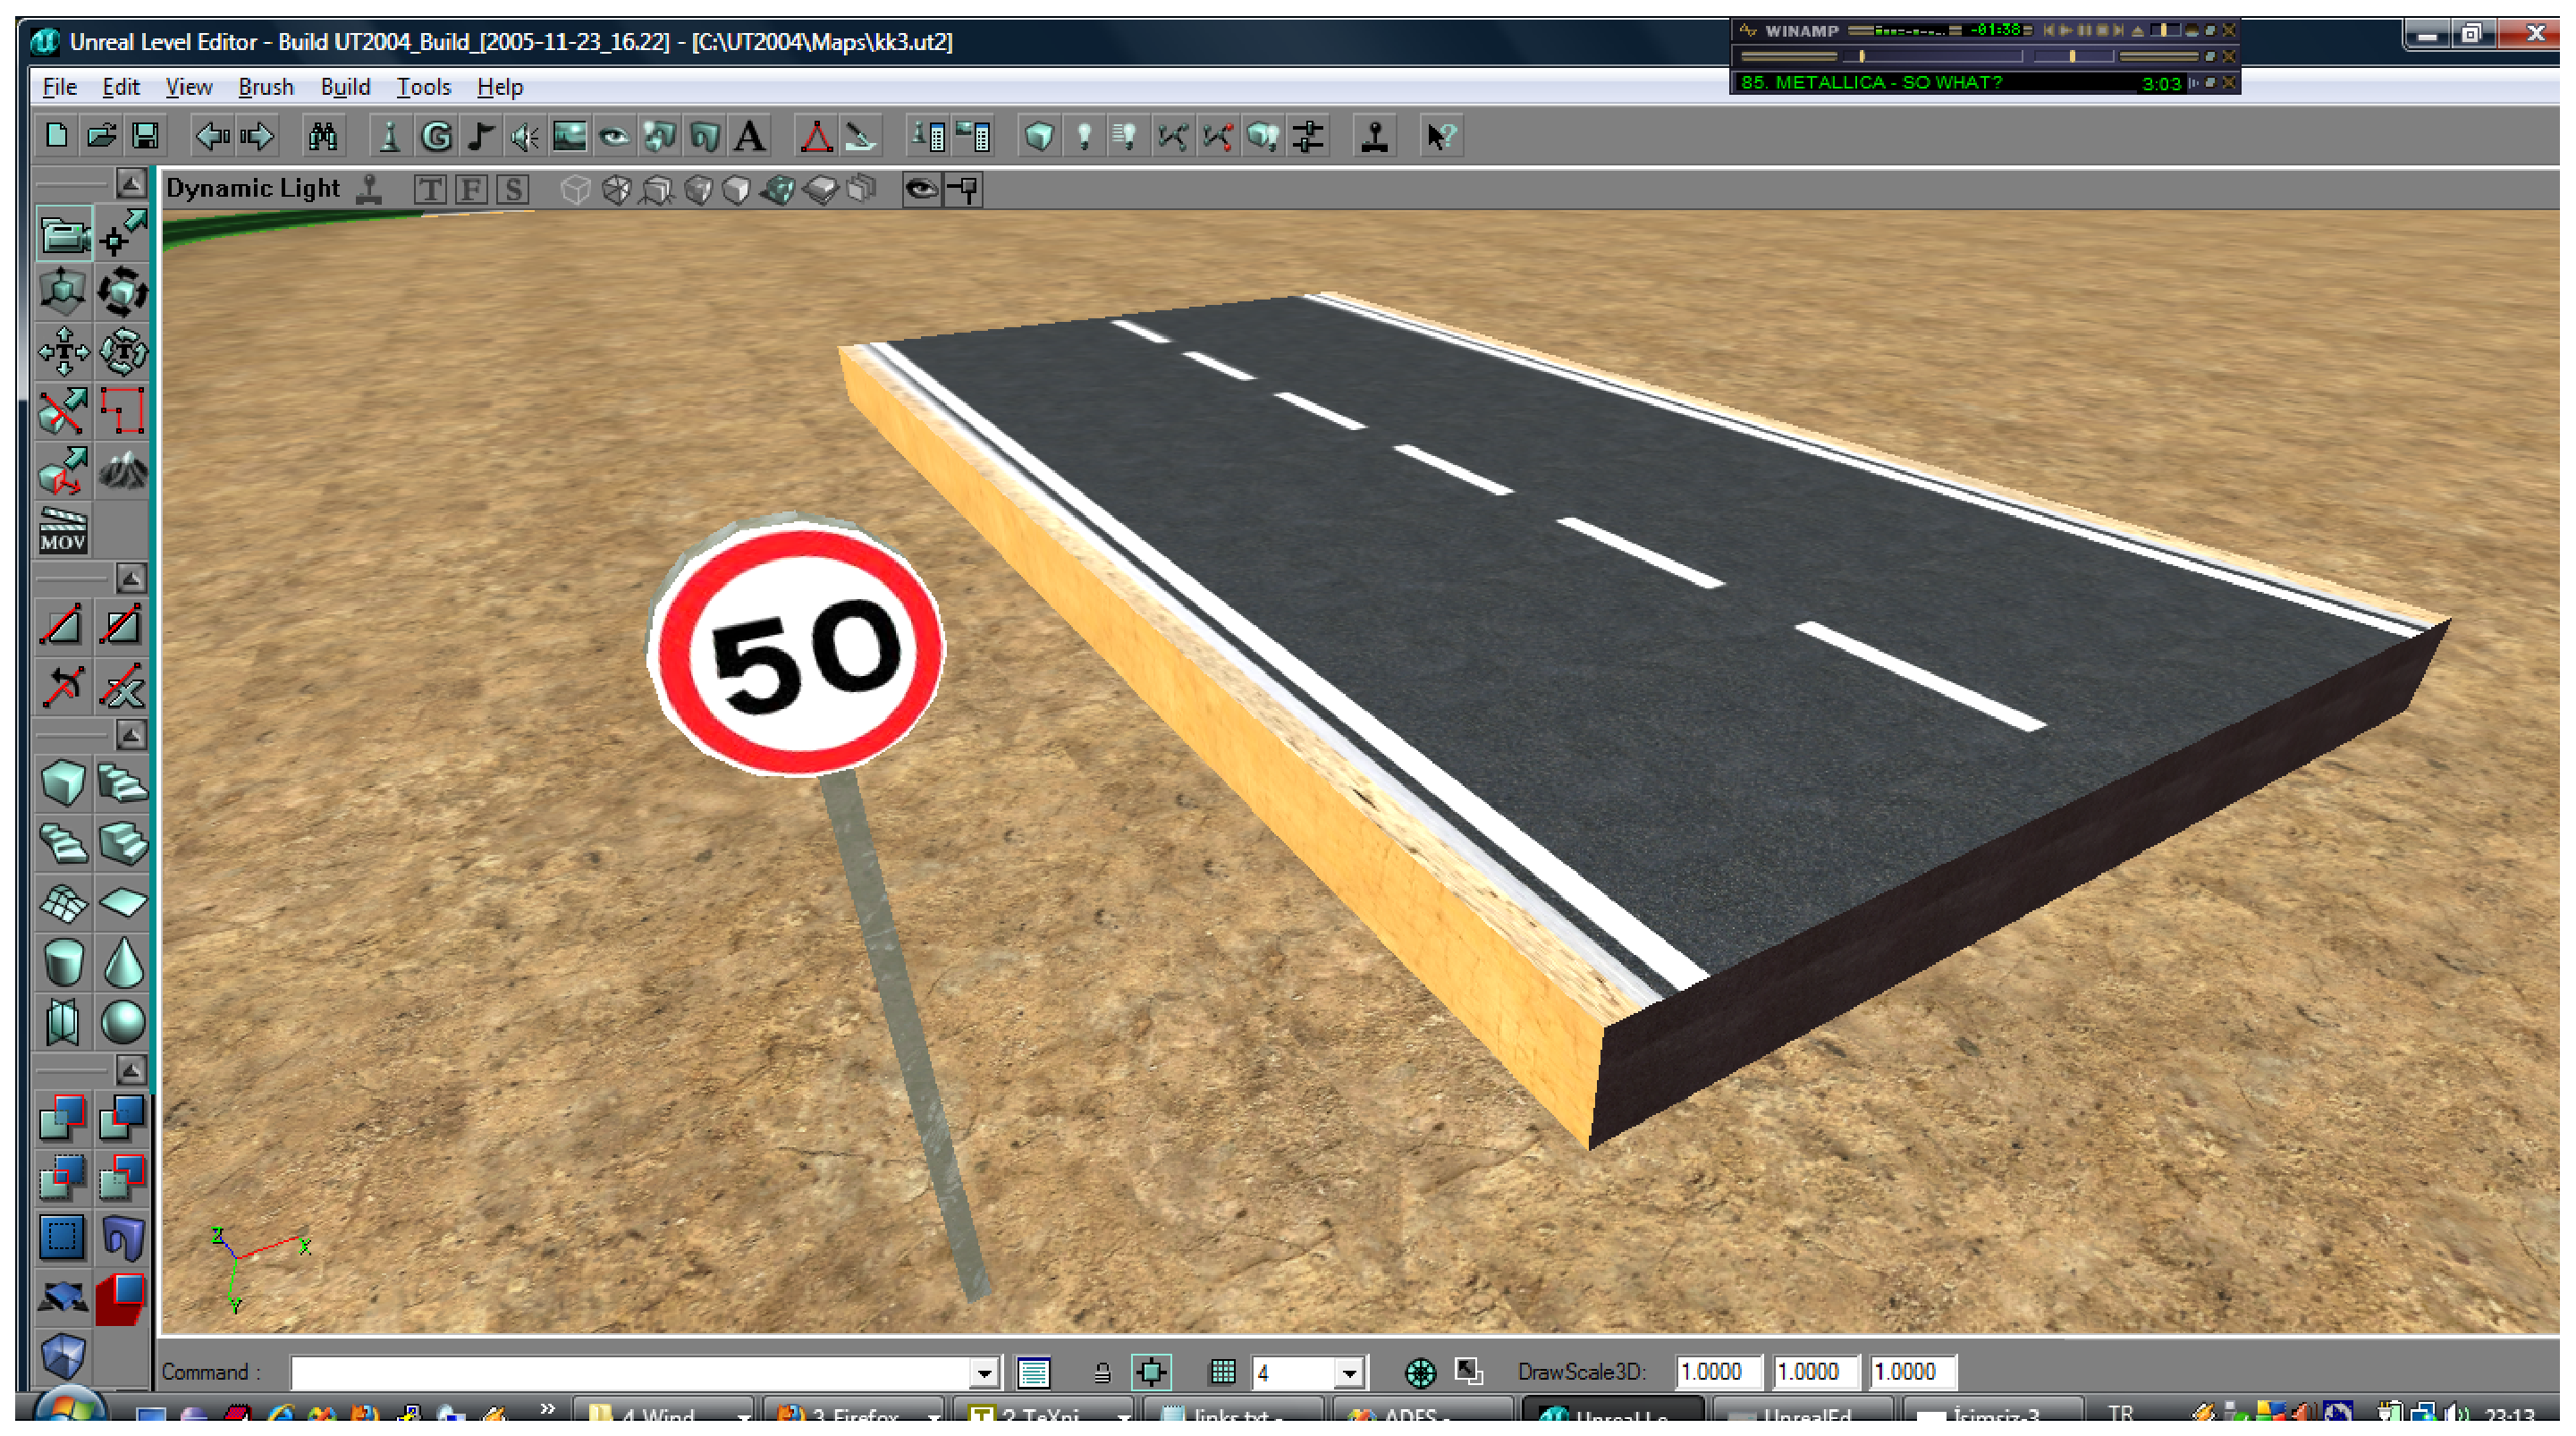
\includegraphics[width=150mm,height=90mm]{img/StaticMesh.eps}
\caption{Road segment and speed limit sign static meshes.}
\label{fig:StaticMesh}
\end{center}
\end{figure}

\subsubsection{Terrain Info}

The TerrainInfo object places a ground structure on the Unreal level. The parameters for the distributions of the random distortions are parametric. In addition, there are various tools for increasing and decreasing the levels of the terrain at specific points. The wireframe representation of the terrain of the ADES Unreal world is given in Figure \ref{fig:Terrain}.

\begin{figure}[ht]
\begin{center}
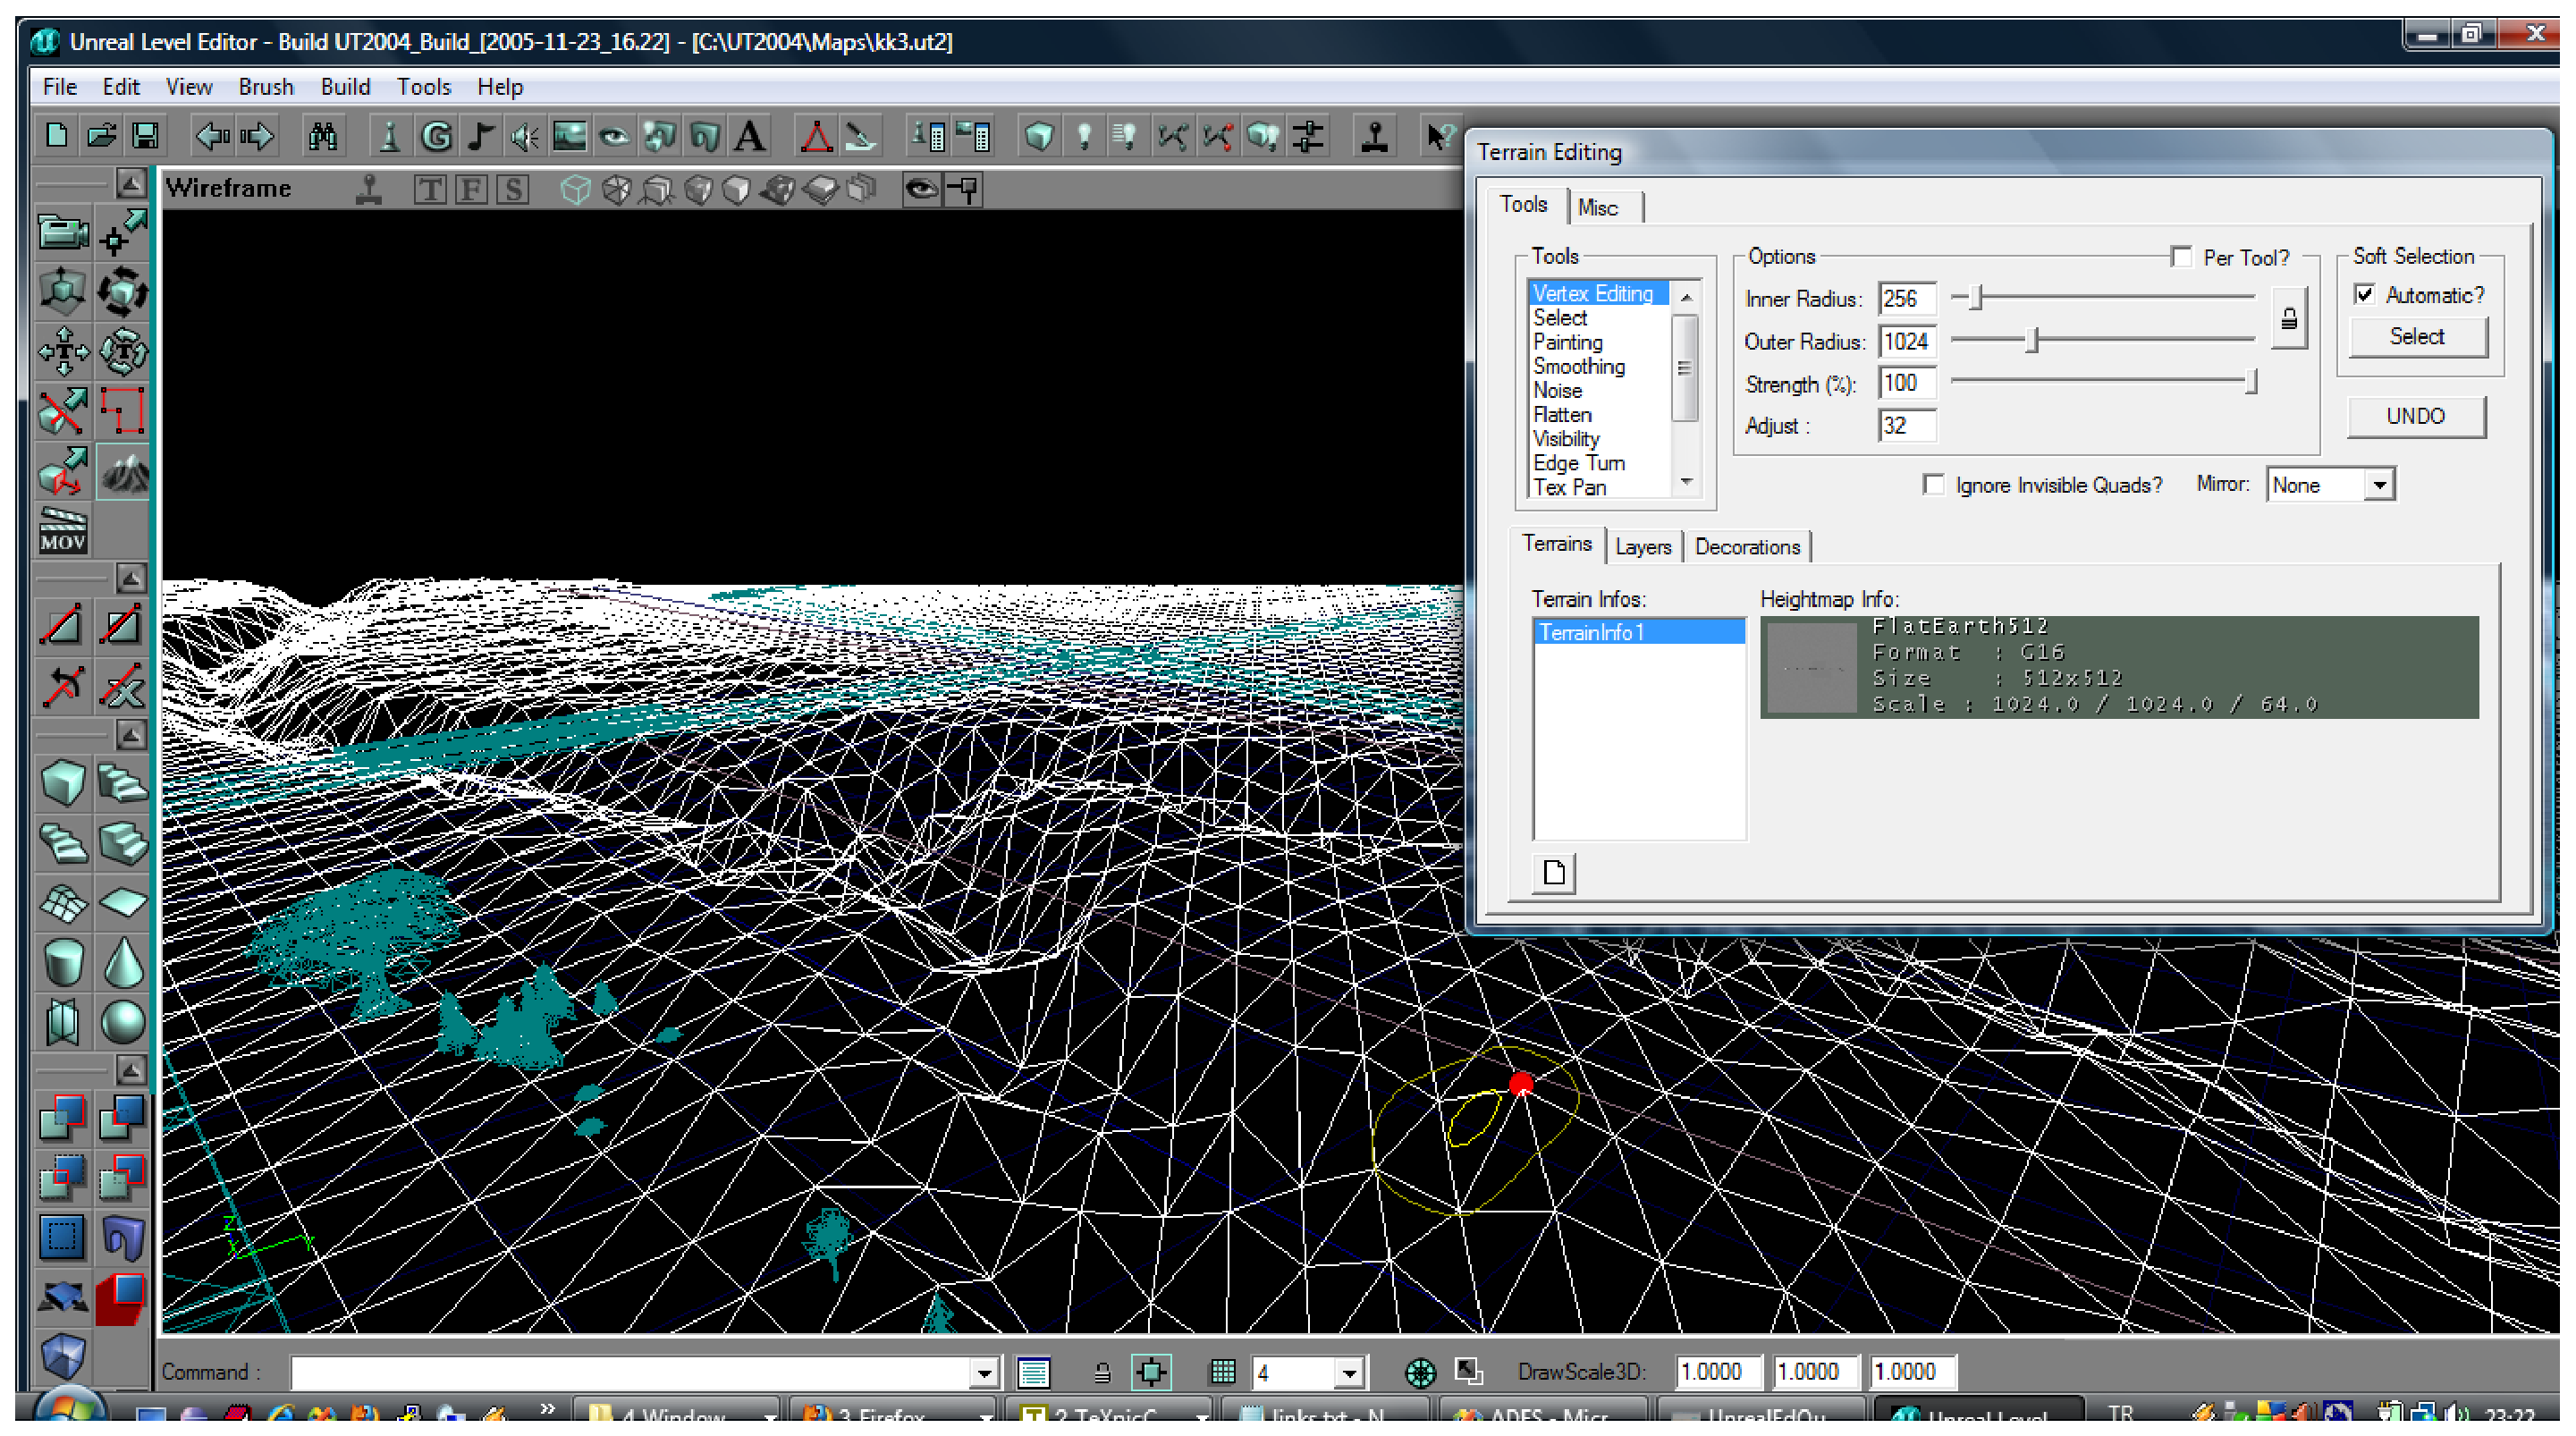
\includegraphics[width=150mm,height=90mm]{img/Terrain.eps}
\caption{The wireframe of the terrain of the ADES Unreal world.}
\label{fig:Terrain}
\end{center}
\end{figure}

\subsubsection{Zone Info}

Miscellaneous properties of the level can be configured by using the ZoneInfo object. The zone lighting, ambient sound effects, fog effects are some of these properties. In addition to the ZoneInfo, different objects derived from Light class can be used for ambient lighting, like SunLight or SpotLight classes.

\subsubsection{Sky Box}

As we mentioned before, the first step of the level design is carving the world as a big rectangle . Initially, the walls of this rectangle which bound our world are empty. The SkyZoneInfo object provides artificial scenes for these walls. This object is placed within a relatively small closed empty space like a cube as shown in Figure \ref{fig:SkyBox}. Then the walls of this smaller empty space are decorated with appropriate wallpapers. Finally, the walls of the bigger rectangle is set as \textit{Fake Backdrop} which is a setting in \textit{Surface Flags}.

\begin{figure}[ht]
\begin{center}
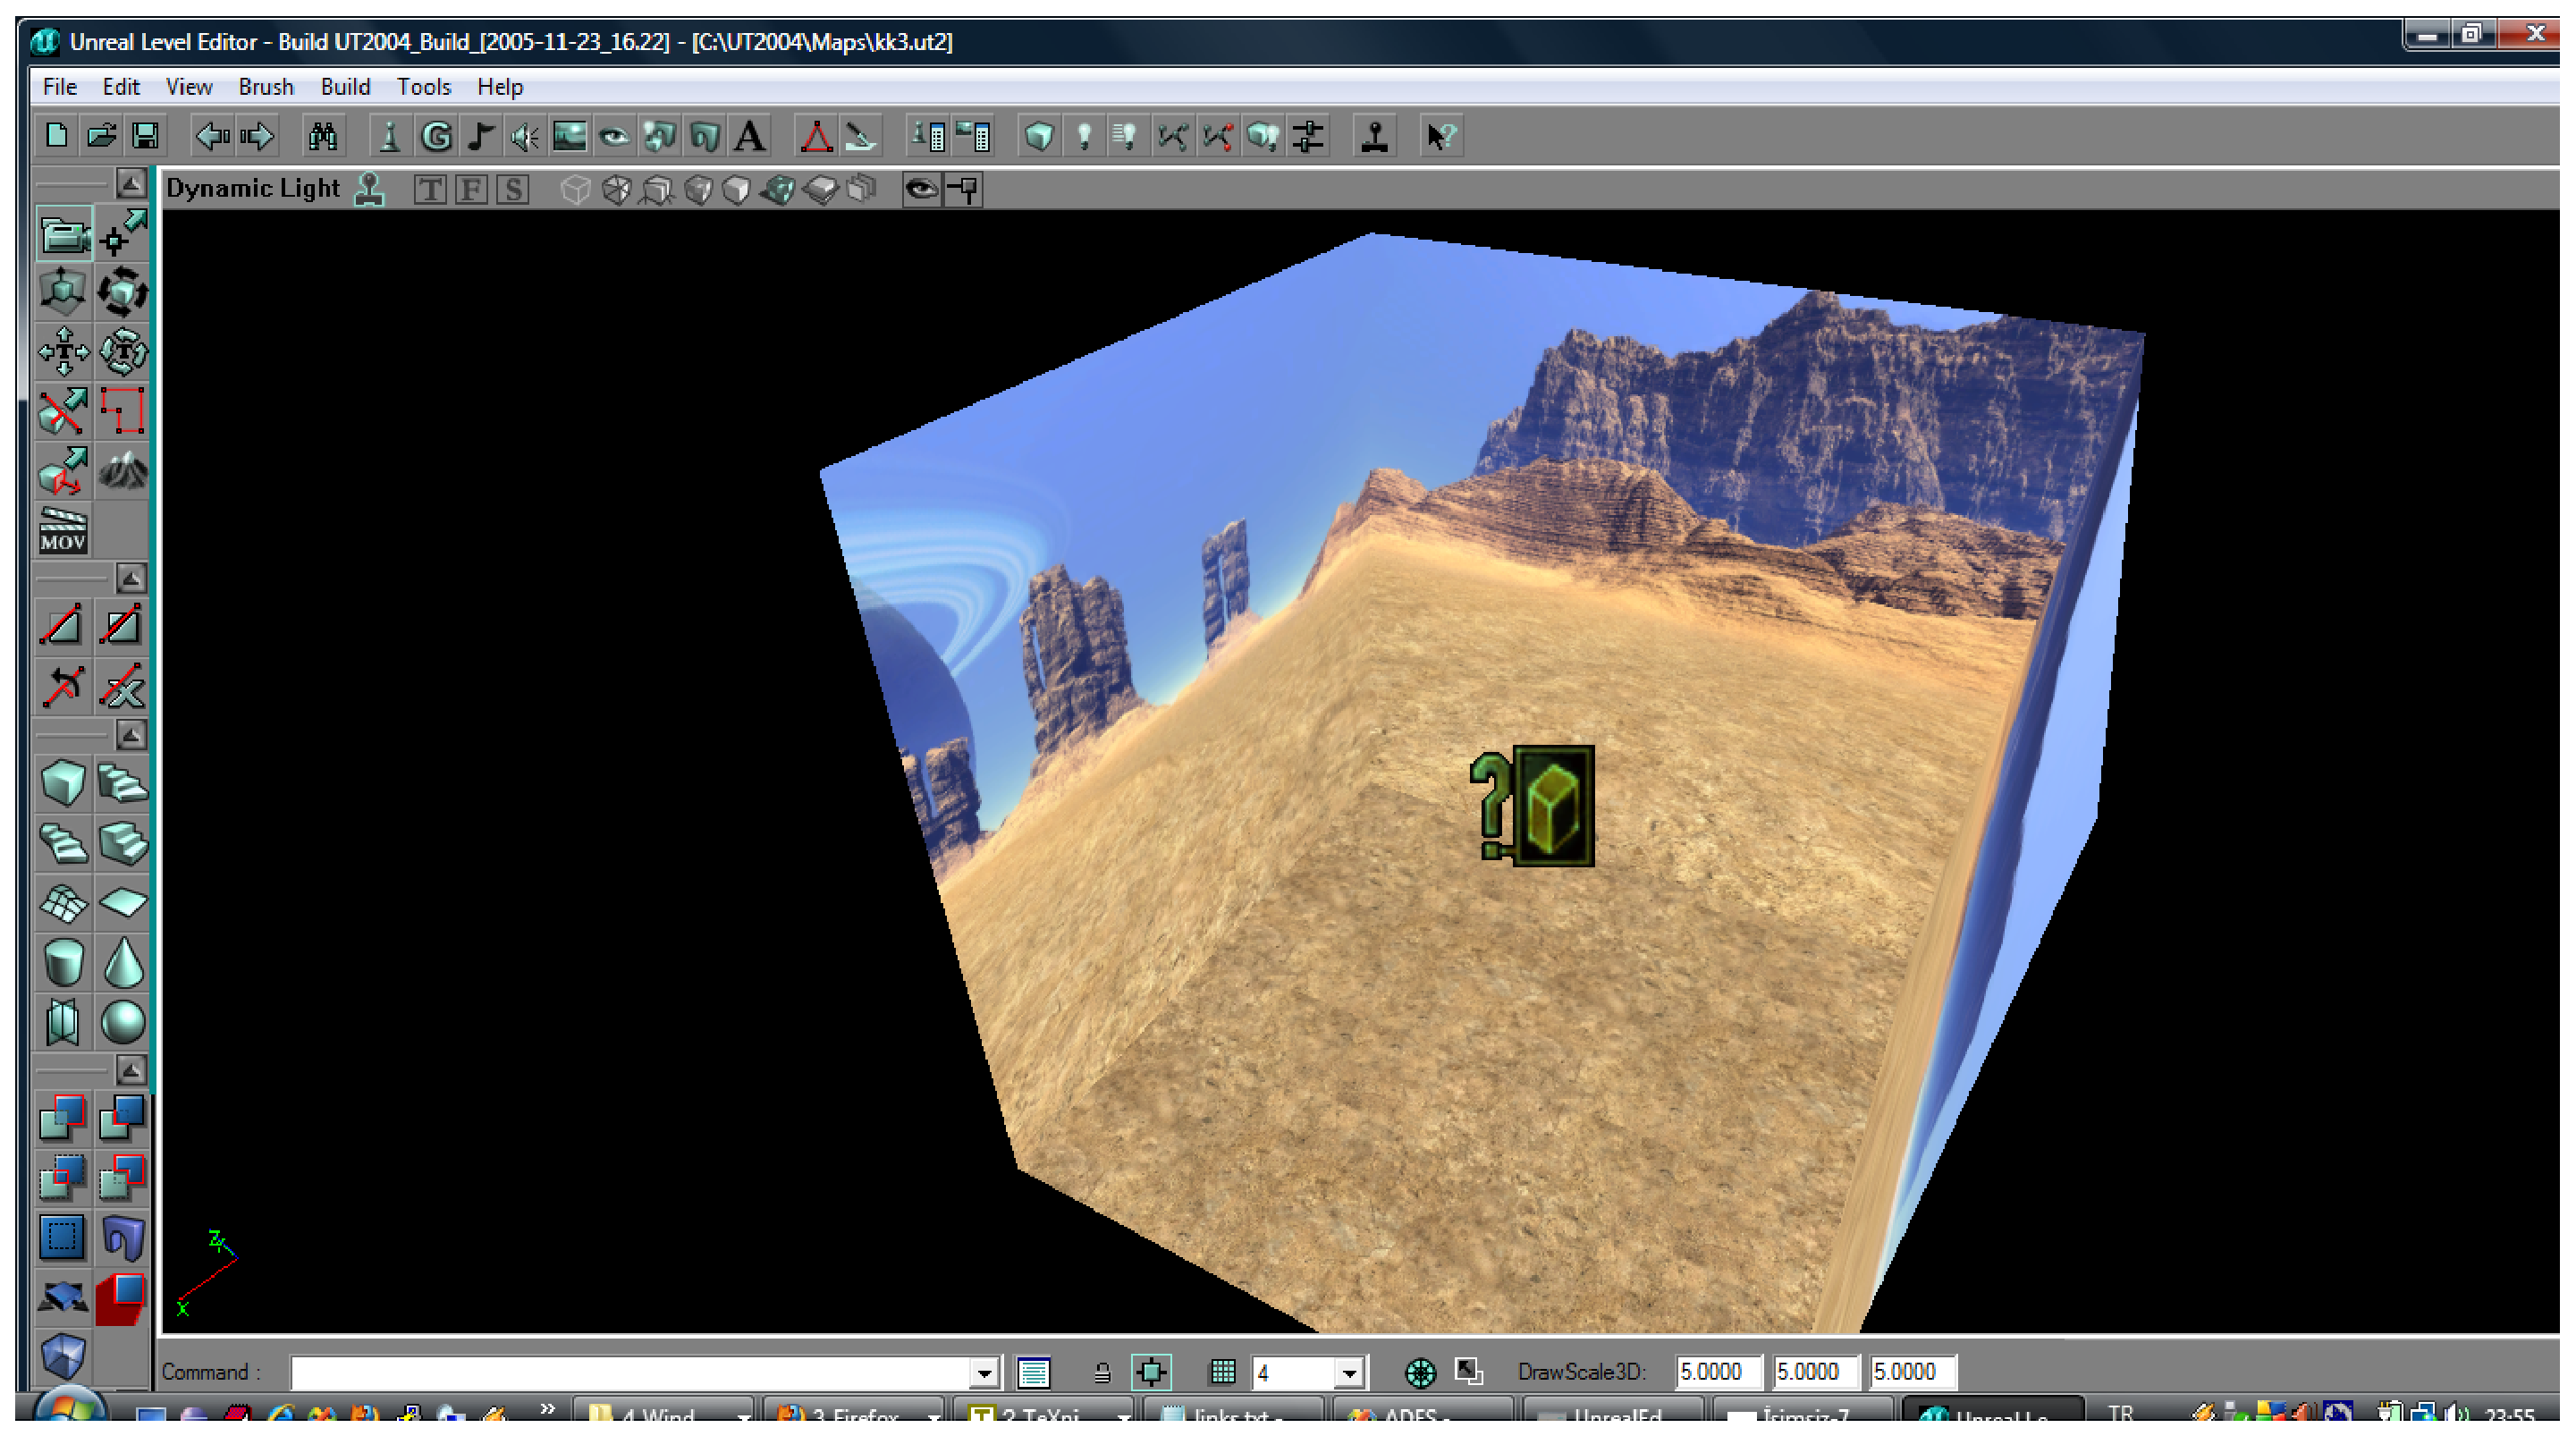
\includegraphics[width=150mm,height=90mm]{img/SkyBox.eps}
\caption{The SkyBox of the ADES Unreal world.}
\label{fig:SkyBox}
\end{center}
\end{figure}

\subsection{UPISEX}

UPISEX is a wrapper project for the USARSim's image server UPIS for making it visible for .NET projects. The main task of this project is creating the Unreal Client with Detours hook. Detours \cite{hunt_detours_1999} is a library for intercepting Win32 functions by re-writing the in-memory code for new target functions. The detoured function call is returned to the intended target after the intercepting function is called. The Detours are used for capturing some of the DirectX \cite{thorn_directx_2005} calls. These calls are branched to the UPIS server which performs additional instructions in order to make the video memory visible to itself. The UPIS server also starts to listen to a specific TCP/IP port to serve those images to the ADES unreal controller.

\subsection{ADES Unreal Controller}

The Unreal Engine provides the simulation environment. USARSim provides various vehicles and sensors that can be reached by outside applications. The UPISEX provides client images to outside applications. The ADES Unreal Controller uses these tools in order to place a vehicle, Sedan, into the ADES Unreal world. Then the human operator controls the Sedan from the application. The application processes the image data and other sensor data and provides facts to its selected expert system. And finally, the expert system is queried after each fact assertion for a traffic violation. If the human operator violates a traffic rule, the application is expected to  warn the operator by providing the type of violation.

\begin{figure}[ht]
\begin{center}
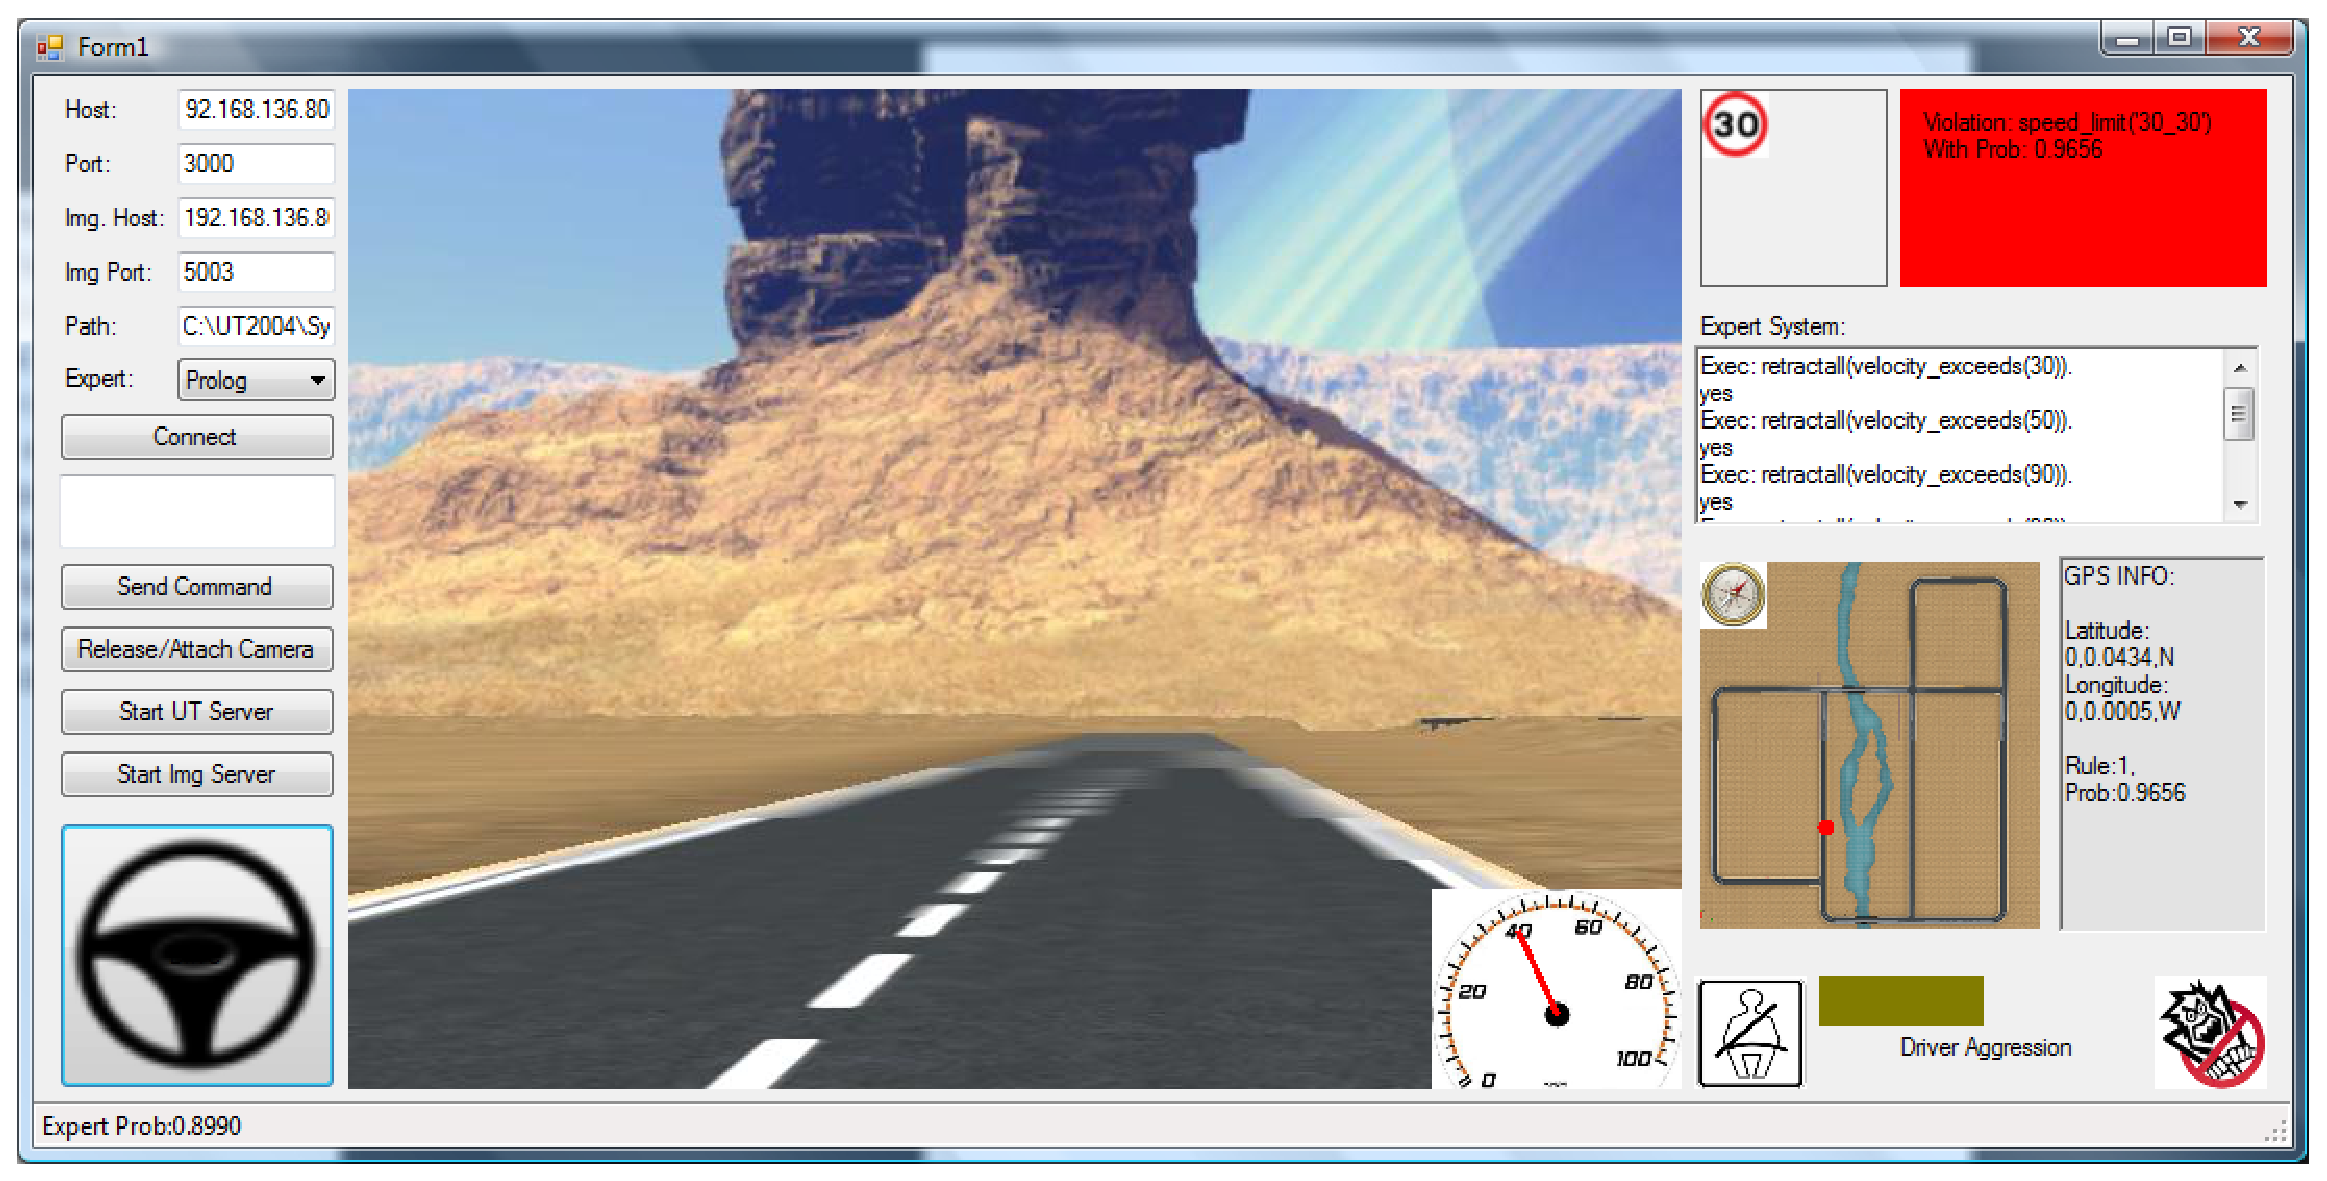
\includegraphics[width=150mm,height=60mm]{img/ADESController.eps}
\caption{The Unreal ADES controller application interface.}
\label{fig:ADESController}
\end{center}
\end{figure}

The application interface is given in Figure \ref{fig:ADESController}. The host and the port is the address of the Unreal Engine. The image host and port is the address of the UPISEX image server. The path is the directory which contains Unreal Tournament 2004 installation. The Expert System selection can be done by using the expert drop down list. The send command button sends the string entered into the white box to the Unreal Engine. The Release/Attach Camera command attaches the client viewpoint to the vehicle's camera or return to the global camera. There are two helper buttons for initiating the Unreal Engine and the USISEX with correct parameters. These applications can also be started from the command line of the target computer.

The panel in the middle of the application displays the image from the UPISEX server. The images can be captured by the vehicle camera or the global viewpoint according to the effective camera in the simulation.

At the right hand side of the camera image, the outputs of different processing can be followed. The detected sign is given in the upper part of the application. The violation box turns to red if a violation occurs. In addition, the details of the violation are also given in this box. The text area below the violation box displays the facts asserted to or retracted from the expert system. Finally, the driver aggression meter is placed at the right bottom of the application.

\subsection{Deprecated Simulators}
Since the framework is developed by using Microsoft's Visual Studio.NET, the first simulation environment considered is Robotics Studio which is also a product of Microsoft company. At the beginning of the project the urban challenge proposed by KIA, which provides a good simulation environment for autonomous urban driving, is available as a research platform. The simulated agent has stereo vision, GPS, bumper detectors and LIDAR sensors. And the actuators are modeled as differential drives for simplicity. However, the company discontinued the simulator which ends our efforts on the environment and the Robotics Studio.
\begin{figure}[ht]
\begin{center}
\includegraphics[width=140mm,height=70mm]{img/inf1.eps}
\caption{KIA Urban Challenge}
\label{fig:inf1}
\end{center}
\end{figure}
\par

\chapter{TESTS AND EVALUATION}
\label{chapter:evaluation}
The ADES project provides an end-to-end framework design and implementation for automatically detecting the traffic violations. To overcome this challenging task various modules are implemented. The performance of these modules are investigated in this section. The presented results are obtained from the real world applications of the proposed system. 

The road lane detection and traffic sign recognition processes are tested on a recorded video sequence of the urban roads in Turkey under different lightning conditions. The video sequence contains more than 150 traffic signs. For the expert system tests, an artificial map created for the simulation environment is used.

\section{Road Lane Detection}
The first solution that will be considered is the road lane detection system, which is a sub-module of the vision system. The average processing time is 21.25 milliseconds for a laptop PC with Intel T2050 processor at 1.6 GHz whereas the average cost of the classical approach is 15.29 milliseconds. The proposed approach managed to detect and track at least one line in most of the sequence. 

\begin{figure}[ht]
\begin{center}
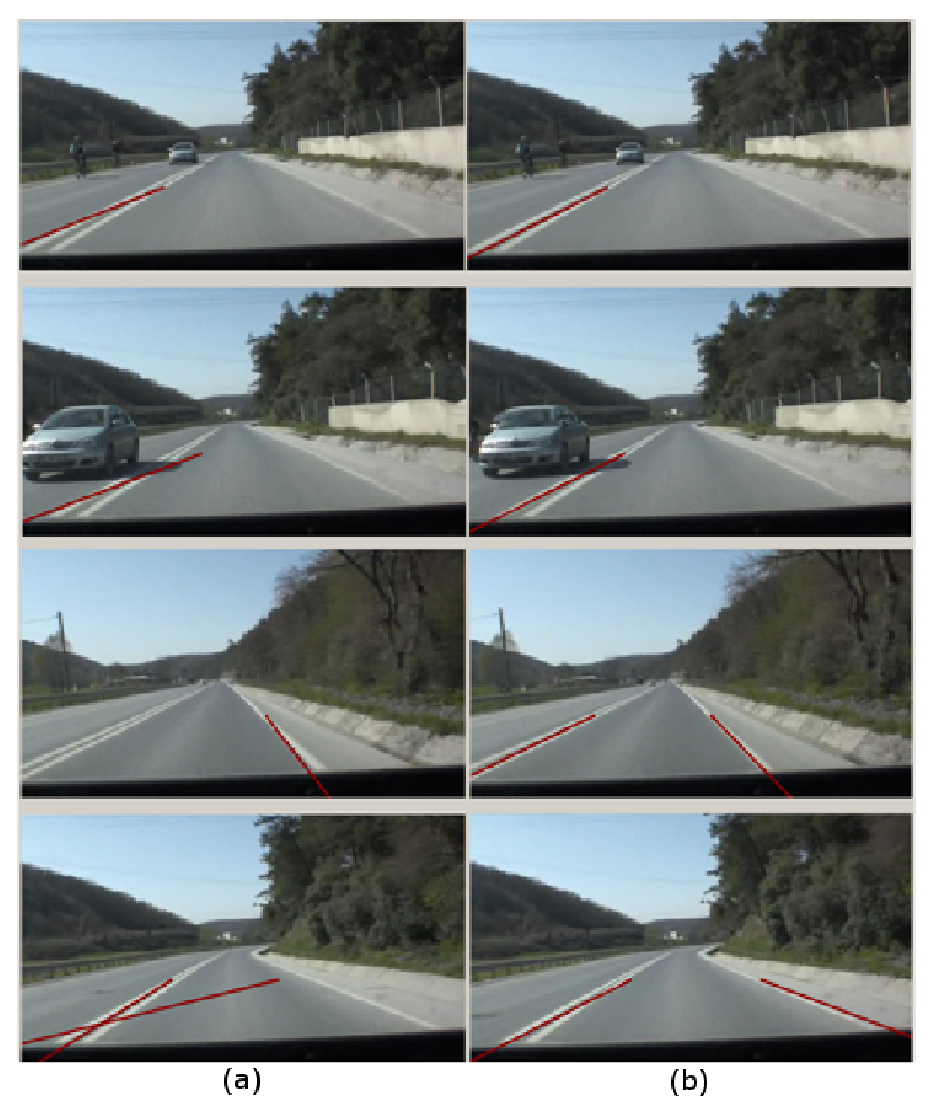
\includegraphics[width=75mm,height=115mm]{img/ldfig4.eps}
\caption{Differences between (a) classical Hough transformation and (b) the proposed approach.}
\label{fig:ldfig4}
\end{center}
\end{figure}
\par

In order to validate the results of the proposed approach, the classical Hough Transform approach is also implemented and the results are compared. In the implementation of the classical approach, the same part of the image is processed using the Hough transform routine without dividing smaller partitions. The most intensive 10 lines are merged according to their \textit{r }and \textit{$\theta $} values. Finally three or less candidate lines are selected as the lane markers. The major differences between the two approaches are shown in Figure \ref{fig:ldfig4}. The images on the left hand side are the detected lines by the classical approach. The right hand side images are the outputs of the new approach for the same frames. The result of this comparison shows that the detection capabilities are increased and the rate of false positives are also decreased by the new approach.

\section{Traffic Sign Detection and Recognition}
The second vision module implemented within the ADES project is the traffic sign detection and recognition system. 

For the detection phase, several measurements are performed. The results are given in Tables \ref{signdetect-table-1} and \ref{signdetect-table-2}. The results show that the system has an efficient CPU time utilization for real life applications. Therefore, it is possible to re-run the whole process more than one hundred times in a second. This gives an opportunity to utilize the GA to track the detected sign over a sequence of frames. For this purpose, half of the best chromosomes at the end of each processed frame are passed to the next frame. 
\par
\begin{table}[ht]
  \vskip\baselineskip
	\caption{Detection rate of circular signs.}
	~\vskip -1mm
	\centering
	\label{signdetect-table-1}
	\begin{tabular}{|l r r r r|}
		\hline
		\textbf{Fitness threshold} 		& 30 & 30 & 30 & 35 \\
		\textbf{Population size} 			& 60 & 120 & 60 & 60 \\
		\textbf{Number of Generations} 	& 2 & 2 & 4 & 2 \\
		\textbf{Mutation rate}     		& 0.35 & 0.35 & 0.35 & 0.35 \\
		\textbf{Crossover rate} 				& 0.75 & 0.75 & 0.75 & 0.75 \\
		\textbf{Selection method} 				& Elitist & Elitist & Elitist & Elitist \\
		\hline
		\textbf{Avg. Process Time(msec)}	& 9 & 14 & 14 & 9 \\
		\textbf{True detections (percent)} &  95 &  96 &  96 &  65 \\
		\textbf{Misses (percent)}	&  5 &  4 &  4 &  35 \\
		\hline
		\textbf{False detections (percent)}				&  5 &  7 &  6 &  1 \\
		\hline
	\end{tabular}
\end{table}
\par
The upper rows of the Tables \ref{signdetect-table-1} and \ref{signdetect-table-2} show the parameter sets, while the lower rows (painted in gray) show the experiment results. \textit{True detections} correspond to the correctly detected signs, whereas the \textit{misses} are the signs that could not be detected at all. Note that, the sum of the true detections and misses is always 100 percent. \textit{False detections}, on the other hand, are the cases where the system indicates a sign existence even though there exists no sign in that location. \textit{False detection rate} is calculated by comparing the number of false detections with the total number of real traffic signs in the video. The first column of values in the tables, is the preferred set of parameters for both the circular and the triangular cases. 
\par
For the circular signs, a fitness threshold of 30, GA population size of 60 and 2 generations yields the ideal results in terms of accuracy and CPU time. It is possible to enhance the accuracy up to 96 percent by increasing either the population size or the number of generations. But this will almost double the processing time for a very small accuracy enhancement, hence is not worth the trade-off. The fitness threshold, on the other hand, has considerable effect on the accuracy, as seen on the rightmost column.
\par
The triangular sign process yields the ideal results with a fitness threshold of 16. That is due to the different geometric characteristics of the triangular signs. The \textit{true detection} rate degrades from 95 percent to 87 percent. It is possible to increase this value by decreasing the fitness threshold from 16 to 12. But this has a side-effect of increasing the false detections from 4 percent to 9 percent.

\begin{table}[ht]
  \vskip\baselineskip
	\caption{Detection rate of triangular signs.}
	~\vskip -1mm
	\centering
	\label{signdetect-table-2}
\begin{tabular}{|l r r r r|}
\hline
\textbf{Fitness threshold} 		& 16 & 16 & 16 & 12 \\
\textbf{Population size} 			& 60 & 150 & 60 & 60 \\
\textbf{Number of Generations} 	& 2 & 2 & 6 & 2 \\
\textbf{Mutation rate}     		& 0.35 & 0.35 & 0.35 & 0.35 \\
\textbf{Crossover rate} 				& 0.75 & 0.75 & 0.75 & 0.75 \\
\textbf{Selection method} 				& Elitist & Elitist & Elitist & Elitist \\
\hline
\textbf{Avg. Process Time(msec)}			& 9 & 16 & 14 & 9 \\
\textbf{True detections (percent)}				& 87 & 88 & 90 & 94 \\
\textbf{Misses (percent)}				&  13 & 12 & 10 & 6 \\
\hline
\textbf{False detections (percent)}				&  4 &  4 &  5 &  9 \\
\hline
\end{tabular}
\end{table}

In the classification phase, Tables \ref{signclassify-table-1} and \ref{signclassify-table-2} exhibit the classification results on \textit{"properly detected"} signs. 

\begin{table}[ht]
  \vskip\baselineskip
	\caption{Classification success rate of circular signs.}
	~\vskip -1mm
	\centering
	\label{signclassify-table-1}
\begin{tabular}{|l r r|}
\hline
\textbf{Classification Method} & NN & SVM \\
\hline
\textbf{Avg. Process Time(msec)}			& 5 & 10 \\
\textbf{Error rate (percent)}				& 9 &  20 \\
\hline
\end{tabular}
\end{table}

\begin{table}[ht]
	\vskip\baselineskip
	\caption{Classification success rate of triangular signs.}
	~\vskip -1mm
	\centering
	\label{signclassify-table-2}
\begin{tabular}{|l r r|}
\hline
\textbf{Classification Method} & NN  & SVM  \\
\hline
\textbf{Avg. Process Time(msec)}			& 3 & 6 \\
\textbf{Error rate (percent)}				&  7 &  9 \\
\hline
\end{tabular}
\end{table}

Table \ref{signdetection-overall} depicts the overall system performance, considering the detection and classification steps as a whole.  The errors of the detection step have an adverse effect on the classification process. For both circular and triangular signs, NN with $12 \times 12$ grid features have yielded the best results in terms of CPU time and error rate. The visual results of the experiments and the related data set can be found on the project web site \cite{kaplan_ades_2009}.

\begin{table}[ht]
  \vskip\baselineskip
	\caption{Overall system performance.}
	~\vskip -1mm
	\centering
	\label{signdetection-overall}
\begin{tabular}{|l|r r|}
\hline
& \multicolumn{2}{c|}{CIRCULAR} \\
\hline
\textbf{Classification Method} & NN & SVM \\
\hline
\textbf{Avg. Process Time(msec)}			& 14 & 19 \\
\hline
\textbf{Error rate (percent)}				&  14 &  24 \\
\hline

\hline
& \multicolumn{2}{c|}{TRIANGULAR} \\
\hline
\textbf{Classification Method} & NN & SVM \\
\hline
\textbf{Avg. Process Time(msec)}			& 12 & 15 \\
\hline
\textbf{Error rate (percent)}				&  11 &  13 \\
\hline
\end{tabular}
\end{table}

The comparison of the sign recognition system with existing systems developed in the last decade is given in Table \ref{tab:perf}. It can be seen that the overall accuracy of the system with NN classification is comparable if not better than the other approaches. Additionally,  the processing time of each frame is smaller than any of the approaches even without considering the differences in the platforms.

%\begin{sidewaystable}
\begin{table}
\vskip\baselineskip
\caption{Comparison of the Proposed Approach with selected methods from the last decade.}
~\vskip -1mm
\centering
\label{tab:perf}
{\scriptsize
\begin{tabular}{|p{19mm}|p{15mm}|l|l|r|r|r|}
\hline
{\bf Method} & {\bf Reference} & {\bf Year} & {\bf Hardware} & {\bf Image Size (px)} & {\bf Time (msec)} & {\bf Success Rate (\%)} \\
\hline
Matching Pursuit &        Hsu and Huang~\cite{hsu_road_2001}&       2000 &   Intel P2 &    512x480 &       ~250 &   up to 88 \\
\hline
Genetic Algorithm &   Escalera \textit{et al}~\cite{de_la_escalera_road_1997}&       2002 & AMD Duron 1Ghz &    384x286 & ~450 (51x8.8) &        N/A \\
\hline
Kalman Filter &       Fang \textit{et al}~\cite{chiung-yao_fang_road-sign_2003}&       2003 & Intel P4 1GHz &    320x240 &      $>$1000 &        N/A \\
\hline
Feature Extraction &        Gao \textit{et al}~\cite{gao_recognition_2006}&       2005 &   Intel P3 &  1680x1680 &       ~450 &   up to 95 \\
\hline
       SVM &     Maldonado-Bascon \textit{et al}~\cite{maldonado-bascon_road-sign_2007}&       2005 & Intel P4 2.2Ghz &    720x576 &      $>$ 1000 &   up to 93 \\
\hline
Geometric Fragmentation &   Soetedjo and Yamada~\cite{soetedjo_traffic_2005} &       2005 & Intel P4 2.6 GHz &    240x180 &       ~750 &   up to 86 \\
\hline
Haar Wavelet Features &   Bahlmann \textit{et al}~\cite{bahlmann_system_2005}&       2005 & Intel Xeon 2.8Ghz &    384x288 &       ~100 &         85 \\
\hline
Neural Networks &      Nguwi and Kouzani~\cite{nguwi_automatic_2006}&       2006 & Pentium M 1.7Ghz &        N/A &       ~550 &   up to 95 \\
\hline
  Adaboost &       Baro \textit{et al}~\cite{baro_traffic_2009}&       2007 &        N/A & 60x60 stereo &      $>$ 1000 &      87-90 \\
\hline
Color Distance Transform &       Ruta \textit{et al}~\cite{ruta_real-time_2010}&       2007 &        N/A &    640x480 &        ~35 &   up to 85 \\
\hline
Affine Trans., GA, NN & Proposed Approach &       2010 & Intel T5450 1.66Ghz &    512x288 &        ~13 &         87 \\
\hline
\end{tabular}  
}
\end{table}
%\end{sidewaystable}

\section{Expert Systems}
Unlike the sensor processing modules, the performance criteria of the inference engine does not depend on the execution time or accuracy. The proposed expert system implementations should be complete and easy to maintain in order to make correct judgments about the drivers' actions. 

Outputs of the proposed expert systems for a speed violation scenario are given in Figure \ref{output}. In both examples the proposed system detects the speed violation after the required facts are provided by the sensors. In the Prolog based expert system implementation, the facts are asserted to the knowledge-base. The expired facts are also retracted from the knowledge-base before any query for the violation is done. On the other hand, in the BN based expert system, the probabilities of the related state are arranged according to the probability of the acquired sensor data. At any time during the execution of this expert system, the sum of the probability values of a specific node should be one.


\begin{mylisting}
Prolog based expert system
\vspace*{2pt}\hrule
\begin{verbatim}
Exec: assert("1.0000::T::sign_detected(speed_limit,30)").
Exec: retractall(velocity_exceeds(X)).
Exec: retractall(velocity_exceeds(50)).
Exec: assert("1::T::velocity_exceeds(50)").
Exec: violation(V,A,P).
Exec: retractall(gps_node_property(speed_limit,30)).
Exec: assert("0.9577::T::gps_node_property(speed_limit,30)").
Exec: retractall(velocity_exceeds(X)).
Exec: retractall(velocity_exceeds(50)).
Exec: assert("1::T::velocity_exceeds(50)").
Exec: violation(V,A,P).
P = 0.957698767978062
V = speed_limit
A = '50_30'
\end{verbatim}

BN based expert system
\vspace*{2pt}\hrule
\begin{verbatim}
SpeedLimit:Vehicle_Speed()->(0,1,0,0)
SpeedLimit belief: 0.5436
SpeedLimit:GPS_Node_Property()->(0.0333333,0.0333333,0.0333333,0.9)
SpeedLimit:Sign_Detected()->(1,0,0,0)
SpeedLimit:Vehicle_Speed()->(0,1,0,0)
SpeedLimit belief: 0.5436
SpeedLimit:GPS_Node_Property()->(0.9708,0.00973333,0.00973333,0.00973333)
SpeedLimit:Vehicle_Speed()->(0,1,0,0)
SpeedLimit belief: 0.9491
\end{verbatim}
\end{list}\caption{Speed violation outputs of proposed expert systems.}
\label{output}
\end{mylisting}

In order to validate the probabilities of the detected violations, the formulation of the probability calculations for both systems should be examined. The probability calculation of the Prolog based system is given in Equation \ref{eq13}
\begin{equation}
\label{eq13}
	p_{v} = (p_{d} \times \alpha_{d} )(p_{s} \times \alpha_{s} )(p_{g} \times \alpha_{g})
\end{equation}
\noindent where $p_{v}$ is the probability of the violation. $p_{d}$, $p_{s}$, and $p_{g}$ are the certainty of velocity reading from the car, the detected sign, and the GIS information respectively. In the current implementation, all facts in the knowledge-base are valid for a predefined time period. The $\alpha$ values are the decaying factors of the related fact. For the given example the small difference between the multiplication of the detection probabilities and the violation probability is due to the time elapsed. Although it is not easy to verify the exact probability of the violation, the multiplication of the detection probabilities gives an upper bound for the violation probability. According to the performed experiments and measurements, the time complexity of the Prolog based expert system is O(n.log(n)). The predicate list for the proposed four violations are queried in less than 10 milliseconds. 

However, artificially asserted 400 rules for violation predicate are queried at nearly 3500 milliseconds. Although the measured execution times are feasible for real time operation in the proposed system, improvements should be considered if the number of violation rules are increased.

The calculation of the violation probability for the BN based expert system is somewhat more complicated. The probability assessments introduced by the human expert should be considered while calculating the violation probability. For the given example the violation probability is calculated by Equation \ref{eq14}
\begin{equation}
\label{eq14}
	p_{v} = \sum_{d\in{Sign\_Detected},s\in{Vehicle\_Speed},g\in{GPS_Node_Property}}p_{d} \times p_{s} \times p_{g} \times vp(d,s,g)
\end{equation}
\noindent where then definitions of $p_{d}$, $p_{s}$, and $p_{g}$ are as explained previously, $vp(d,s,g)$ is the predefined probability assessment value at the $yes$ state of the violation node for the detected sign, velocity and GPS node. And finally, the $s$, $d$, and $g$ elements are the states of the corresponding node in the BN graph. For the previous example, the violation probability is calculated in the Equation \ref{eq15} 
\begin{eqnarray}
\label{eq15}
p_{v} &=& 0.9708 \times 1 \times 1 \times 0.9570 \\
\nonumber & & + 0.00973 \times 1 \times 1 \times 0.7660  \\
\nonumber & & + 0.00973 \times 1 \times 1 \times 0.7870  \\
\nonumber & & + 0.00973 \times 1 \times 1 \times 0.5110  \\
\nonumber p_{v} &=& 0,94913832
\end{eqnarray}
\noindent where the last multiplicand of each line is the probability assessment value for the violation node. Please note that the lines with zero $p_{d}$ and $p_{s}$ values are omitted for readability. The belief network calculation may differ for other traffic regulations due to the structure of the network. For example, since the post nodes in directional regulations depend on pre nodes, a similar calculation should be performed for the post nodes before finding the violation probability.

As a result of the implementations performed on the simulation environment, it can be seen that the proposed expert system implementations do not require extensive efforts for constructing and maintaining. This is due to the simplicity of the existing traffic rules. However, for more complicated rules the performance of the system depends on the human expert who introduces the predefined rules to the inference engine.

\chapter{CONCLUSION AND RECOMMENDATIONS} 
\label{chapconc}
The social and economic impact of the traffic accidents are increasing every day. Fortunately the number of institutes and efforts to prevent traffic accidents and compensate their damages are also increasing day by day. Most of the countries develop their traffic safety programs according to the 4E's of safety which are engineering, enforcement, education, and emergency. Engineering step deals with the conditions of roads and highways, proper settlements of signs and other traffic indicators. Education step is the proper public access to the basic rules and important knowledge about traffic. Emergency part is the planning and improvement of the actions which should be taken after an accident occurs. And the enforcement step adapts the road traffic legislation and the way it is enforced. Since most of the accidents are caused by the drivers, education and enforcement becomes more important for preventing the traffic accidents. 	

\section{The Main Conclusions}

In the ADES project we addressed the problem of developing an application framework for automatic detection of the violations performed by the drivers. The problem is considered in two main sections. The first section is the acquisition  of the raw data from different sensors and processing these data to obtain the valuable information which can be transferred to the inference engine. Although there are numerous kinds of sensors available in the market, we focused on camera, RF reader and GPS devices since these devices that are relatively easy to obtain and already used by various systems in the industry. The algorithms used in the vision system are tested upon real images where the RF and GPS systems are modeled in the simulation environment. The second section of the problem is the design of the inference engine. The rules of data flow between the sensors and the inference engine are defined by an interface which should be implemented by any candidate expert system. The valuable information acquired from the sensors are introduced to the inference engine as facts. The inference engine uses its internal rules and definitions plus these facts to make a judgment about the actions of the driver. The final decision of the inference engine is output by the system with adequate details.

Although this problem is not addressed before in the literature, to the best of our knowledge, there are many applications of ADAS systems are on the market. The aim of the ADES project \textbf{is not} to compete with these implementations. On the contrary, our aim is to present a framework where these enhancements can easily be plugged in. This modularity requires a flexible system design where abstraction should be carefully utilized in the software.
The integration of various ADAS systems to the proposed solution requires implementation of a flexible and easy to maintain expert system. The proposed expert system tries to identify the challenges on the way and present feasible solutions to these problems. The presented expert system implementations give examples of both rule based and probabilistic models. Although the addressed traffic rules are not very complicated, they are the most important regulations for the road safety. In addition, the proposed implementations give a roadmap for extending the system for including other types of the traffic rules. 

The methodology of the proposed system presents various novelties. The selected point based image binarization, the MHT-HMM lane detection, the GA and affine transformation based sign detection mechanism, the RFID and GPS data structures, the enhanced Prolog engine with probabilistic and time-decaying facts, the simulator environment for driver fault detection are all original artifacts of the ADES project.
Finally, the performance of the proposed system with all these enhancements is evaluated to be feasible for the selected purpose. The tests performed in the developed applications shows that the system is capable of detecting traffic violations. Obviously there are some assumptions and prerequisites for performing this challenging task. This is the main reason why we think the ADES project as an developable framework instead of a packaged solution.

\section{Recommendations for Future Work}
The proposed system presents an end-to-end implementation for the simulated environment. Some applications for real environment are also presented. However, there are areas which need more research for the project. The topics for these research areas are,
\begin{itemize}
	\item End-to-end implementation of the application for the real environment: The current state of the project provides an end-to-end solution for the simulation environment. Although the source feed can be easily changed to a real camera input, certain amount of configurations should be performed to set up the system.
	\item Self modifying, or learning, inference engine: The proposed expert systems require predefined rules and assignment to perform their operations. The automation of mining these rules will be a valuable improvement to the proposed system.
	\item Improved sensor processor modules for given modules: Better sensors and better processing algorithms are the inevitable requirements for improving the system. A vision processor which can handle bad weather conditions, or a more precise GPS system will obviously increase the performance of the system.
	\item Integration of advance vision processing modules: Vision is the heart of the system while interacting with the real environment. GPS or RF technologies cannot provide information about the dynamic environment without additional deployments. Therefore the vision data should be processed more intensively to understand the environment. The traffic lights, the pedestrians, other vehicles on the road, unexpected obstacles, signs printed on the roads, and many other features can be extracted from the vision data. The advanced vision processing modules may also be capable of detecting traffic signs in adverse weather conditions.
	\item Wireless integration of the system to the traffic control center: Although the goal of this project is informing the driver about his or her violations, a traffic control center like a police center, can be notified about the drivers actions.
	\item More vehicle to vehicle and vehicle to infrastructure communication: In the near future the vehicles will be more intelligent and possess various means to communicate with their environments. The proposed system may benefit from this communications by obtaining more information about the environment. For example, if a vehicle detects a sign it can broadcast this information to the other vehicles.
	\item Integration with existing intelligent highway systems: In most of the advanced cities there are already deployed traffic control mechanisms. Integration with these systems may be useful for both parties.
\end{itemize}	
\appendix\chapter{ADES Software Design Documentation}
This design document presents the details of the software implemented for the ADES project. The document follows the guidelines given in the IEEE Computer Society's Recommended Practice for Software Design Descriptions \cite{ieee_computer_society_ieee_1998}. The references and acronyms sections are omitted from the document because these sections are already given in the thesis documentation. However, the document is enriched by the section about the software development methodology.
\section{INTRODUCTION}
\subsection{Scope}
This document contains the design description of the Automatic Driver Evaluation System software. The description contains the architectural features of the proposed system layout where the operations of each implemented module is explained in detail. The primary audience of this document is the software engineer. ADES software provides a library for implementing a framework for processing the data acquired from different sensors. In addition, sample applications for real life and simulated environment examples. The system is developed by the ADES project group of Bo{\u g}azi{\c c}i University Artificial Intelligence Laboratory for research purposes.
\subsection{Document Overview}
This software design description document is organized into the following sections:
\begin{itemize}
  \item Introduction: The scope and the outline of the document is presented.
	\item Decomposition Description: The main modules of the software and their duties are explained.
	\item Dependency Description: The main dependencies of the software is listed.
	\item Interface Description: The details of the user interface for the end user is given.
	\item Detailed Design: The low level details are documented.
	\item Software Development Methodology: The tools and techniques used for the development process are explained.
\end{itemize}

\section{DECOMPOSITION DESCRIPTION}
\subsection{Module Decomposition}
\begin{figure}[ht]
\begin{center}
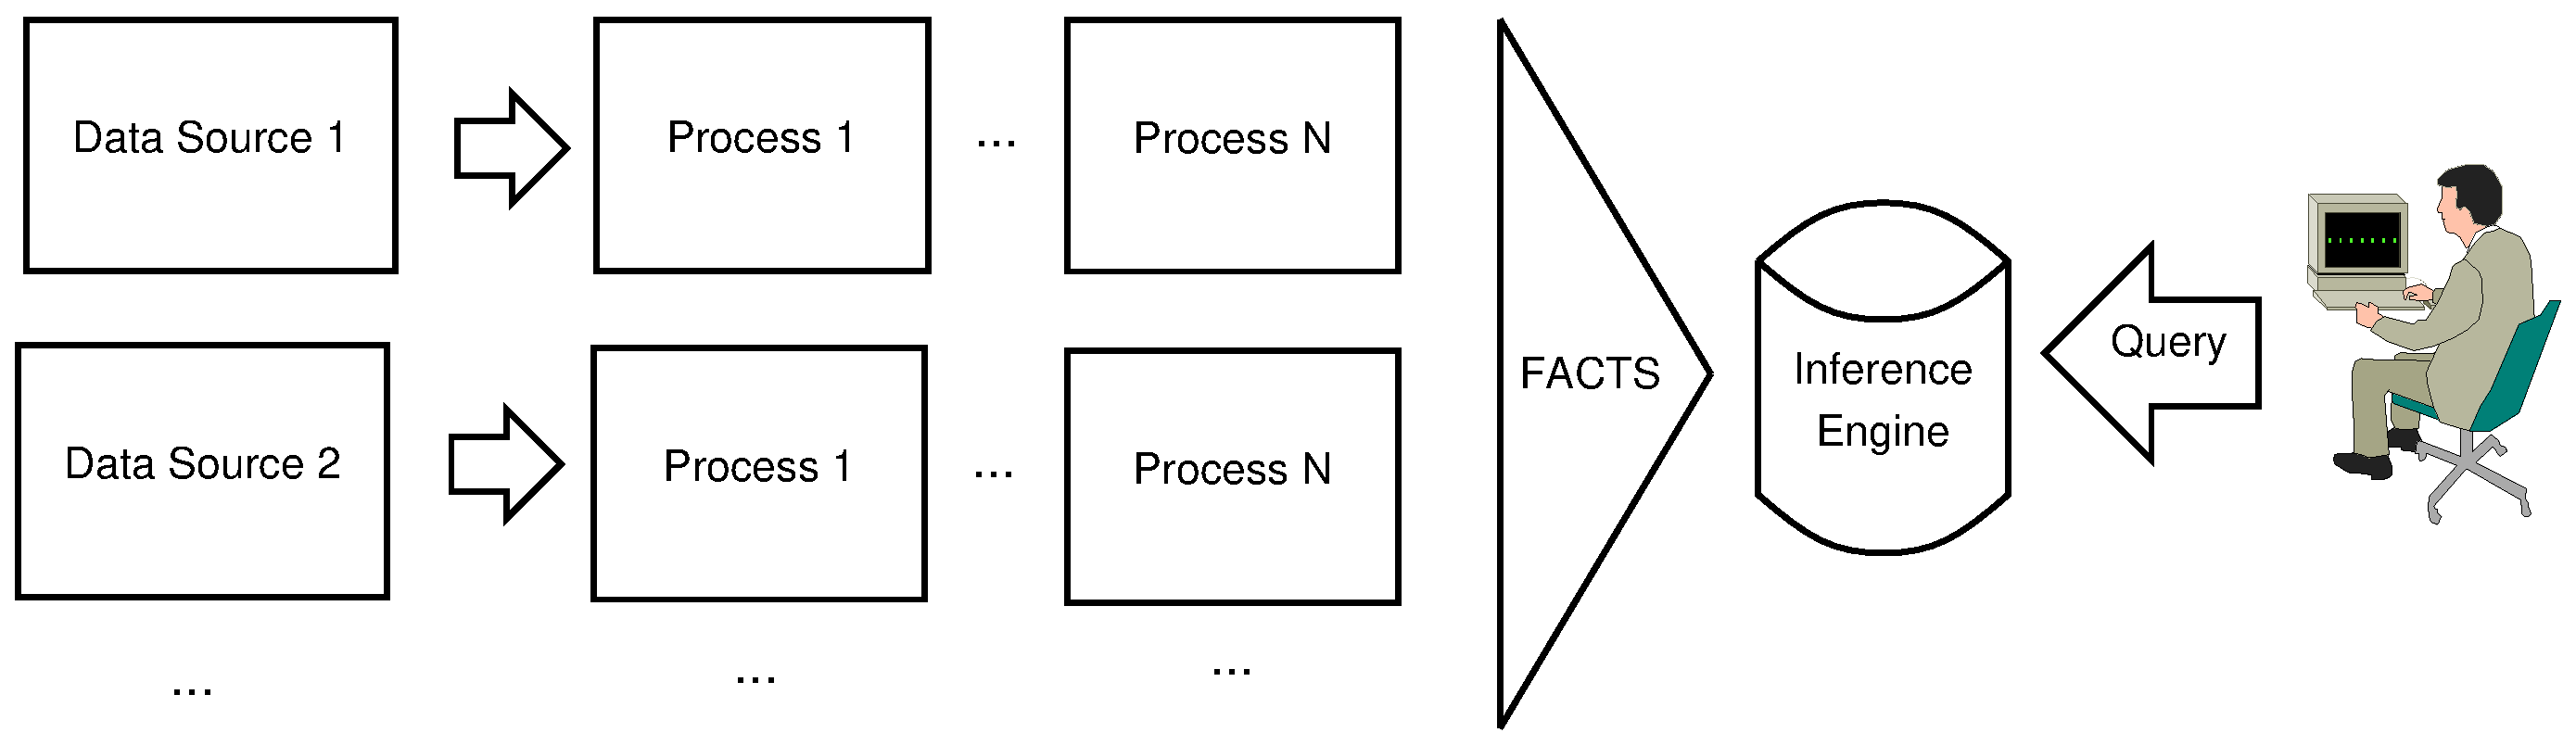
\includegraphics[width=140mm]{img/modulapp.eps}
\caption{The module decomposition of ADES project.}
\label{fig:modulapp}
\end{center}
\end{figure}

The main modules used in the ADES project can be grouped in three categories. The first category contains the source classes derived from message initiator base class which has start and stop features. The source module is responsible for providing information from the outside world to the application.

The second module is the processor layer. There are various processor classes for different purposes. They are all extended from the message consumer base class which has a method for message consuming. All processor classes also provide a function for exposing the message types they can process. This message type is presented in the construction of these classes.

The last module is the inference engine. The proposed expert system implementations for the inference engine should implement the expert system interface as explained in the thesis documentation. 

\subsection{Process Decomposition}
The process decomposition of the project is based on the process implementation classes. The processor classes consumes the messages provided by the source module. The implemented processors are,
\begin{itemize}
	\item HistogramProcessor: Finds the histogram of the captured image for improving the binarization process.
	\item AForgeProcessor: A generic processor for utilizing the AForge image library features.
	\item LaneDetectorProcessor: MHT and HMM base lane detector processor.
	\item CircularSignDetectorProcessor: Processor for detecting circular signs.
	\item TriangularSignDetectorProcessor: Processor for detecting triangular signs.
	\item HoughLineProcessor: Hough line processor for classical lane detection method.
	\item AutoBrightnessProcessor: Automatic brightness correction processor.
	\item SVM\_SURFProcessor: Sign classification processor uses SVM based on SURF features or grid based features.
	\item NN\_Processor: Sign classification processor uses NN based on grid based features.
	\item NN\_SURFProcessor: Sign classification processor uses NN based on SURF features.
\end{itemize}

\subsection{Data Decomposition}
The data flow of the ADES project is controlled by the message flow class. The bindings between the source objects and the processor objects are declared by adding those objects to the message flow. The messaging system provides two types of services. The first one is the basic message service which simply transfers the acquired message to the target object. The second one, which is the message dispatcher, creates a copy of the acquired message for all registered target objects.

The messages implement the message interface which defines the basic requirements for a message object. There are four types of messages in the current implementation of the system. 
\begin{itemize}
	\item Generic Message: Any basic message format. All messages can be converted to this type for serialization purposes.
	\item UDP Message: Carries information in distributed deployments of the processors and source classes.
	\item Vision Message: The basic image information from the source objects.
	\item Text Message: Text based information provided by the source objects.
\end{itemize}

\section{DEPENDENCY DESCRIPTION}

ADES projects depends on several projects. Most of these projects are open source. The brief descriptions of these projects, their usages and web addresses are as follows.

\begin{itemize}
	\item AForge.NET: This is a CSharp framework designed for developers and researchers in the fields of Computer Vision and Artificial Intelligence. Various components of this project is used in the ADES project for implementing neural networks, genetic algorithms and vision processing. The source codes can be achieved from the project home page, which is, \textit{http://www.aforgenet.com}.
	\item Accord.NET: This is another CSharp framework extending the excellent AForge.NET Framework external with new tools and libraries. Accord.NET provides many algorithms for many topics in mathematics, statistics, machine learning, artificial intelligence and computer vision. The Levenberg-Marquardt implementation of this library is used in the ADES project. The web page from the project is \textit{http://accord-net.origo.ethz.ch} where the source codes can be found.
	\item ALGLIB: ALGLIB is a cross-platform numerical analysis and data processing library. It supports several programming languages (C++, CSharp, Pascal, VBA) and several operating systems (Windows, Linux, Solaris). The LDA implementation of the ALGLIB project is used in the ADES project. The project can be accessed at \textit{http://www.alglib.net}.
	\item DirectShowNet Library: The purpose of this library is to allow access to Microsoft's DirectShow functionality from within .NET applications. We used this library to read video files and acquiring live camera images. Detailed information about the project can be found at \textit{http://directshownet.sourceforge.net}.
	\item OpenSURF: OpenSURF is an implementation of SURF (Speeded Up Robust Features) which detects landmark points in an image, and describe the points by a vector. The surf features in the ADES project are detected by the CSharp port of the OpenSurf library which can be found at \textit{http://www.chrisevansdev.com/computer-vision-opensurf.html}.
	\item SVM.NET: This is a .NET conversion of libsvm project, which is is an integrated software for support vector classification, regression, and distribution estimation. The .NET port can be found at {http://www.matthewajohnson.org/software/svm.html}. The project is used for SVM based classification of the traffic signs.
	\item USARSim: USARSim is a high-fidelity simulation of robots and environments based on the Unreal Tournament game engine. The details for the usage of the USARSim library is given in the thesis documentation. The project homepage is \textit{http://usarsim. sourceforge.net}.
	\item CSharpProlog: A CSharp based open source Prolog engine. We modified the engine for implementing the time-decaying facts and the probabilistic facts. The original project can be found at \textit{http://cs-prolog.sourceforge.net/}.
	\item MSBNx: MSBNx is a component-based Windows application for creating, assessing, and evaluating Bayesian Networks, created at Microsoft Research \textit{http://research. microsoft.com}.
\end{itemize}

\section{INTERFACE DESCRIPTION}
\subsection{ADES Detector}
\begin{figure}
\begin{center}
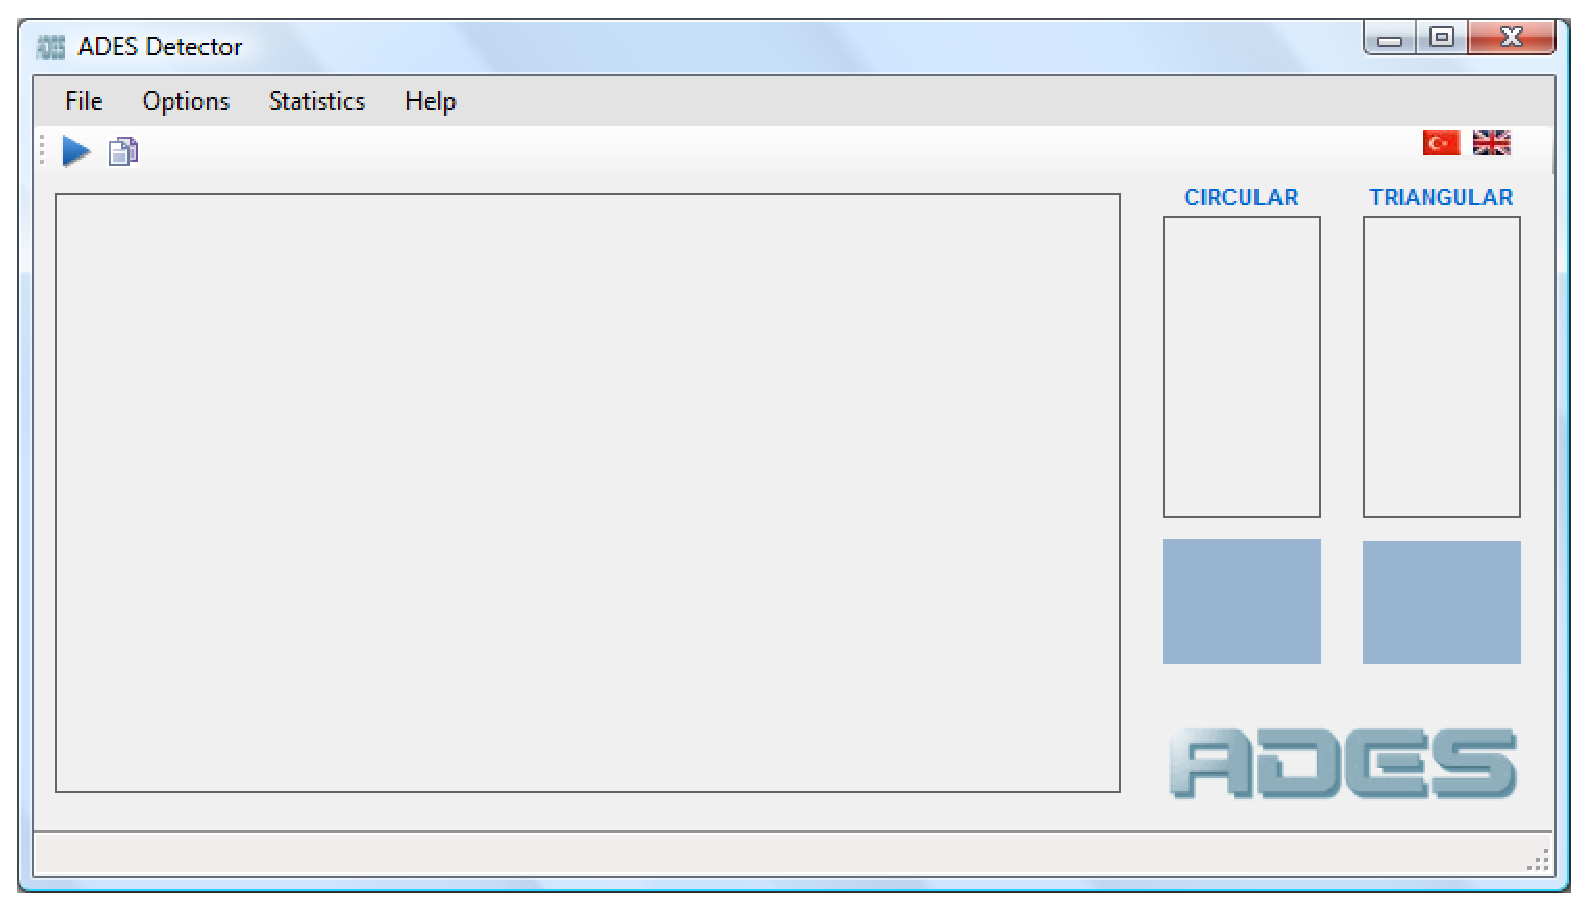
\includegraphics[width=140mm]{img/adesdetectorapp.eps}
\caption{ADES Detector.}
\label{fig:adesdetectorapp}
\end{center}
\end{figure}
The real world tests are performed by the ADES detector application. The menu options of the application are;

\begin{itemize}
	\item File/SVM/Train: Initiates a SVM training process. Options for the training process are defined in Constants class.
	\item File/NN/Train: Initiates a SVM training process. Options for the training process are defined in Constants class.
	\item File/LDA/Generate Feature Array: Selects the most important features according to the LDA analysis.
	\item File/LDA/Use LDA Features: Forces system to use the detected LDA features.
	\item Options/Lane Detection: Invoke lane detection process.
	\item Statistics: Show statistics log file.
	\item Help: Help menu (to be implemented).
\end{itemize}

The buttons on the window are for starting the entire process and dumping the statistic data to the log file. The detected, and recognized signs are displayed at the right side of the window. The detected road lanes are directly drawn within the processed video sequence.

\subsection{ADES Unreal Controller}
\begin{figure}
\begin{center}
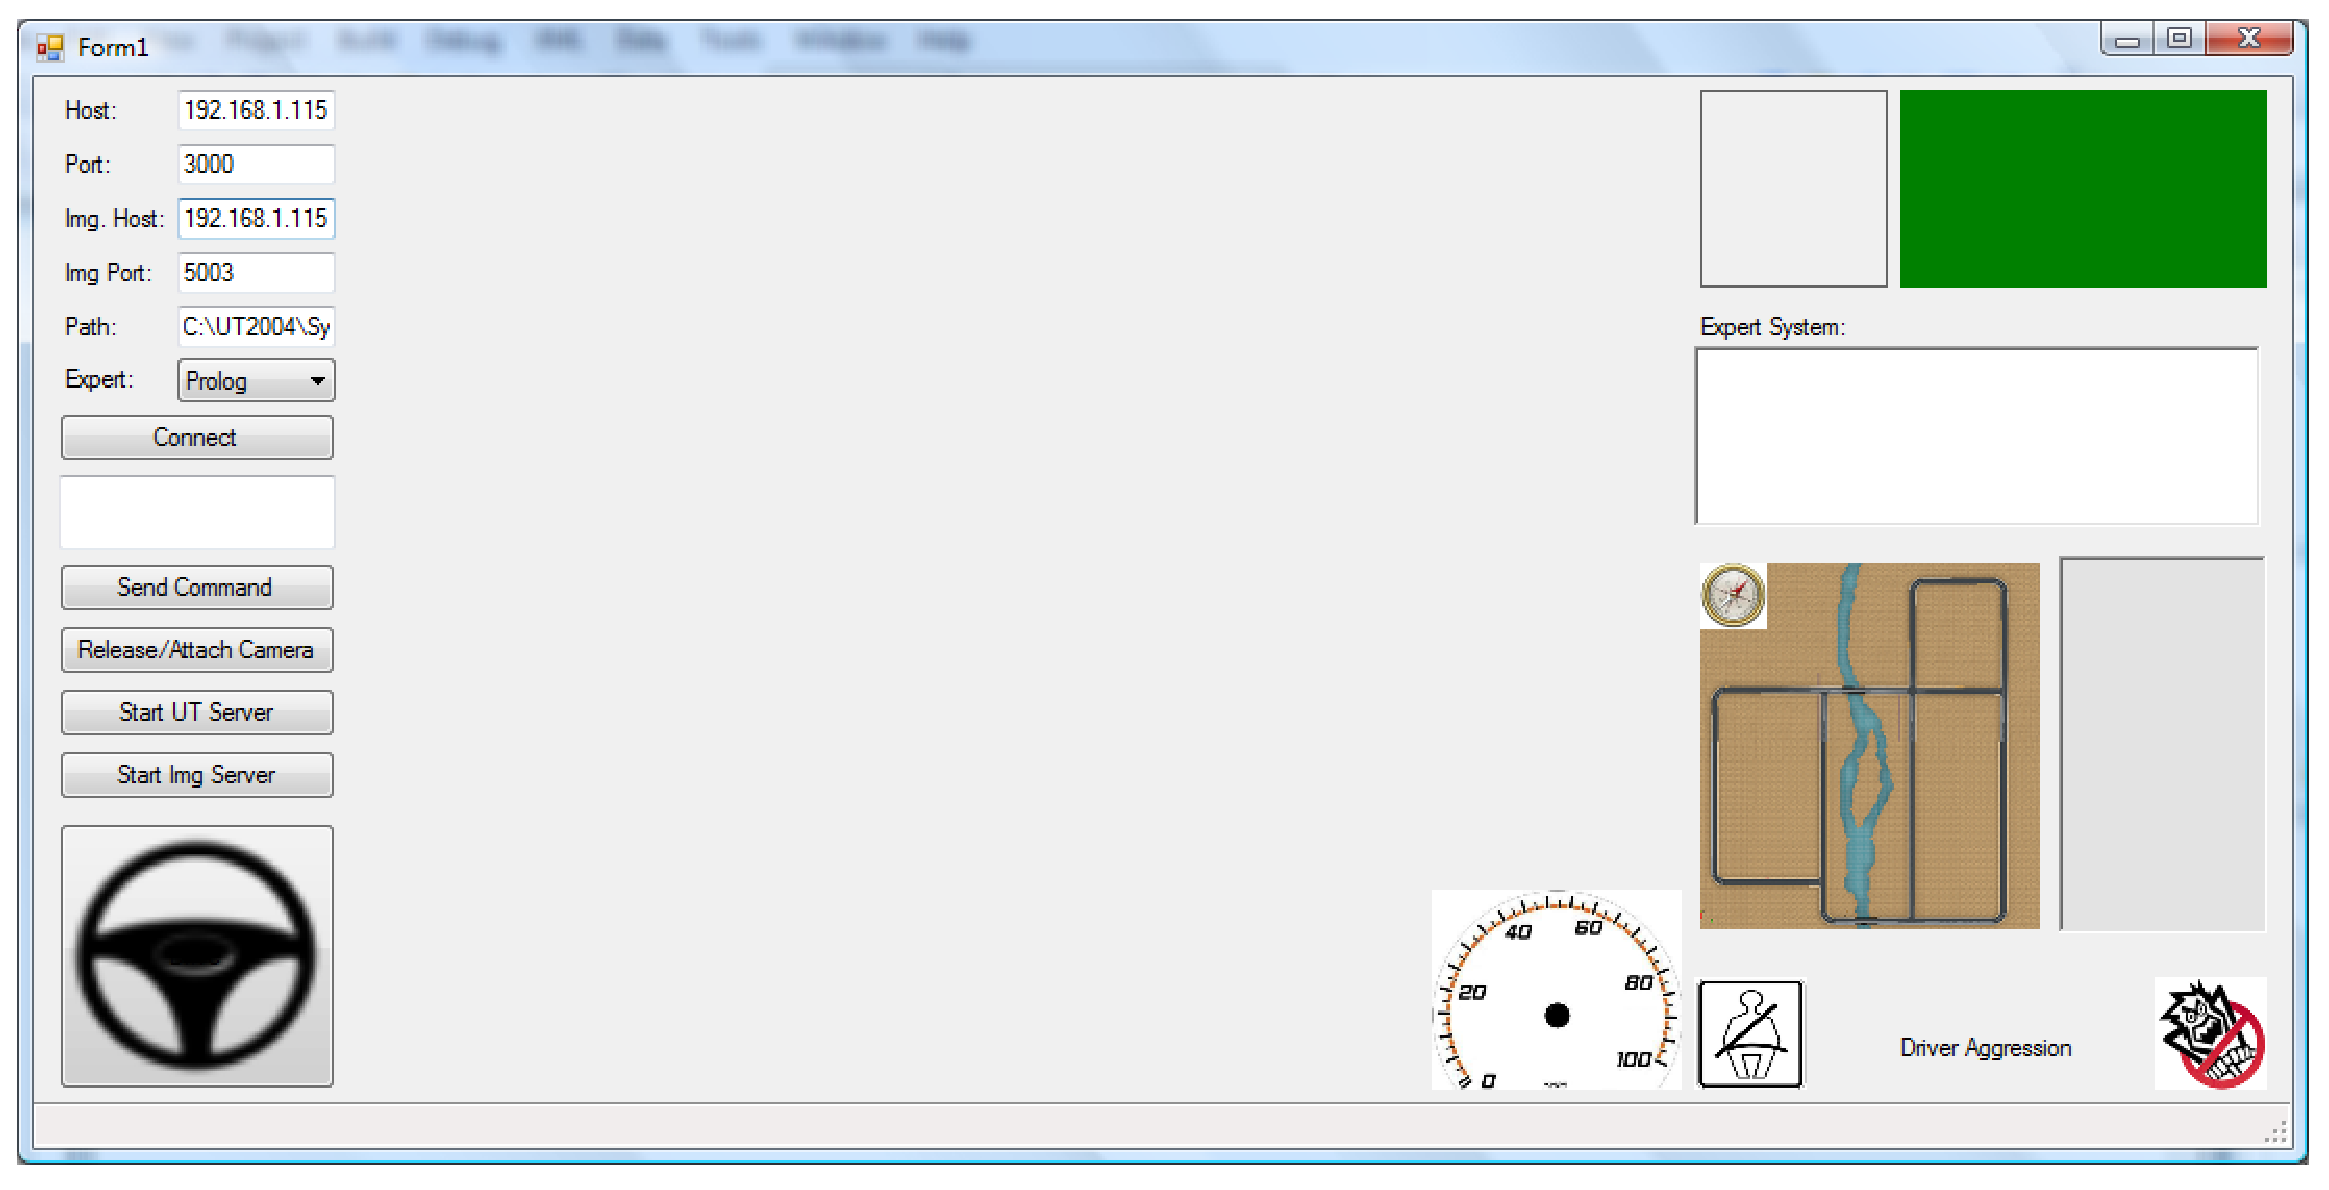
\includegraphics[width=140mm]{img/adesunrealapp.eps}
\caption{ADES Unreal Controller.}
\label{fig:adesunrealapp}
\end{center}
\end{figure}
The ADES unreal controller has a simple but efficient interface for starting the simulation environment and the client application. The definition of the user interface components are,
\begin {itemize}
	\item Host (Text Box): The TCP IP address of the simulation engine.
	\item Port (Text Box): The TCP port of the simulation engine.
	\item Img. Host (Text Box): The TCP IP address of the UPISEX application.
	\item Img. Port (Text Box): The TCP port address of the UPISEX application.
	\item Path (Text Box): The path for the executables of the simulation engine.
	\item Expert (Combo Box):  The expert system should be selected before connecting the agent.
	\item Connect (Button): Spawns a new vehicle agent in the simulation environment.
	\item Unnamed Text Area: Custom USARSim command area.
	\item Send Command (Button): Sending custom USARSim command to the simulation engine.
	\item Release/Attach Camera (Button): Active camera selection. The global camera or the camera attached to the vehicle is selected alternatively.
	\item Start UT Server (Button): Starts the simulation engine.
	\item Start Img Server (Button): Starts the client application.
	\item Steering Wheel (Picture Button): The vehicle can be connected via W, A, S, and D buttons, after the vehicle is connected to the simulation environment.
	\item Speedometer (Picture Box): Displays the speed of the vehicle.
	\item Sign Box (Picture Box): The detected sign.
	\item Inference Result (Colored Label): The result of the violation query from the inference engine.
	\item Expert System (Text Area): The message log for expert system.
	\item Map (Picture Box): The position of the vehicle according to the GPS system.
	\item Unnamed Disabled Text Area: The GPS and GIS information.
	\item Driver Aggression (Progress Bar): Current aggression coefficient of the driver.
\end{itemize}	

\subsection{ADES Sign Recognition Test Utility}
\begin{figure}
\begin{center}
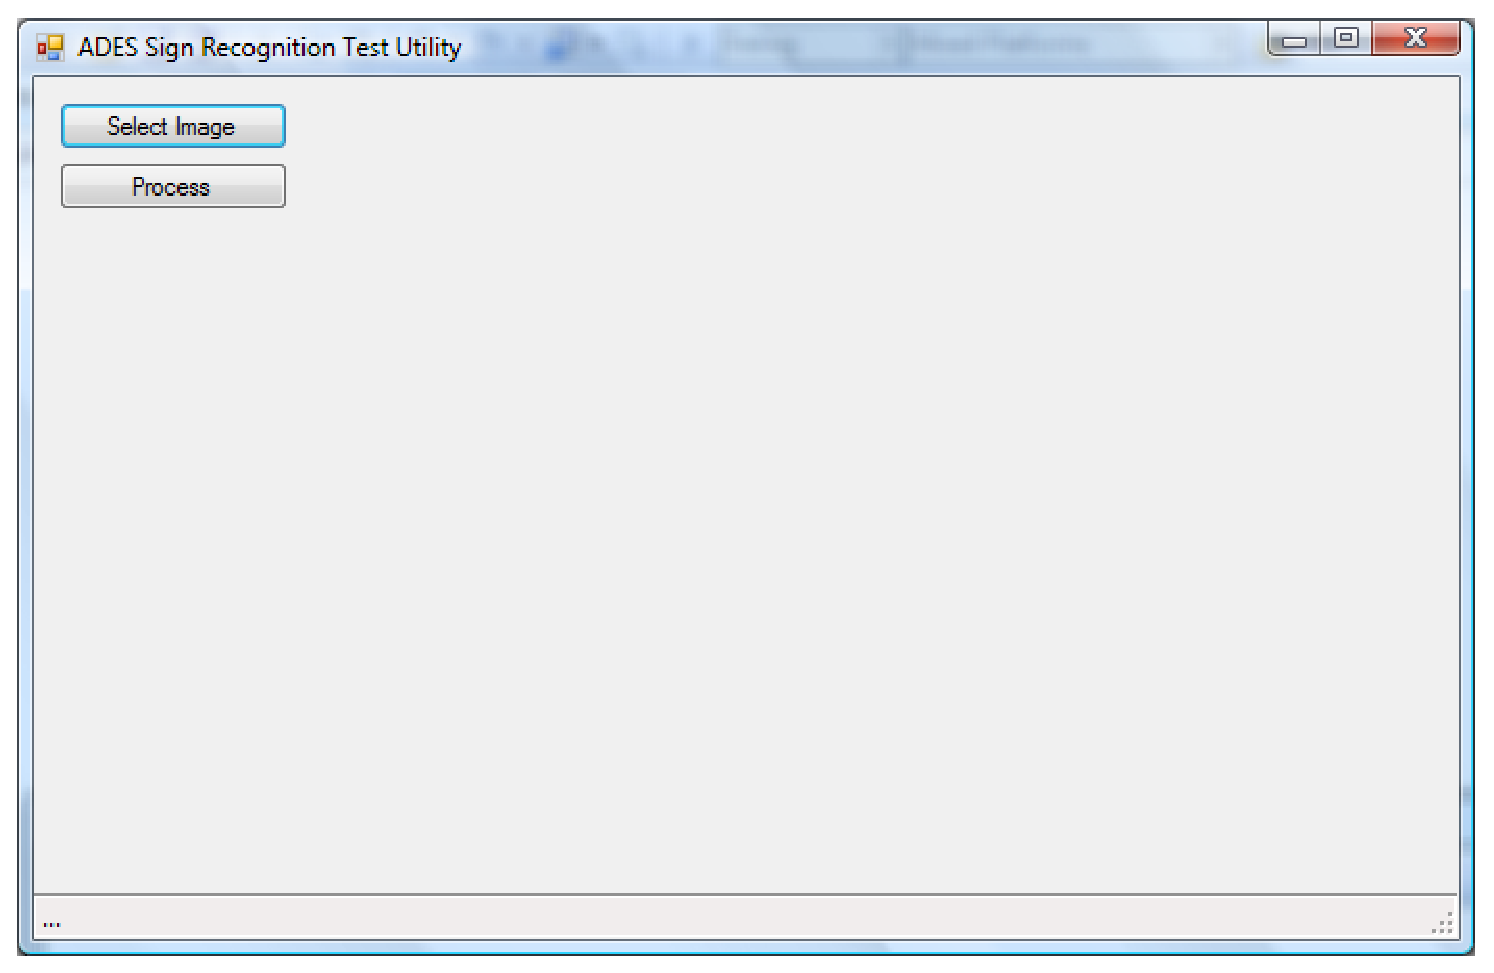
\includegraphics[width=80mm]{img/adestestapp.eps}
\caption{ADES Sign Recognition Test Utility.}
\label{fig:adestestapp}
\end{center}
\end{figure}
A very simple test utility for evaluating the sign recognition strategies is developed. The user simply selects a recorded picture, and initiates the sign recognition process. The system displays the recognized sign at the left of the window, it manages to detect a traffic sign.

\section{DETAILED DESIGN}
The entire class hierarchy diagram of the ADES project is given in Figure \ref{fig:cdapp}. Please note that some utility classes are removed from the diagram for simplicity.
\begin{figure}
\begin{center}
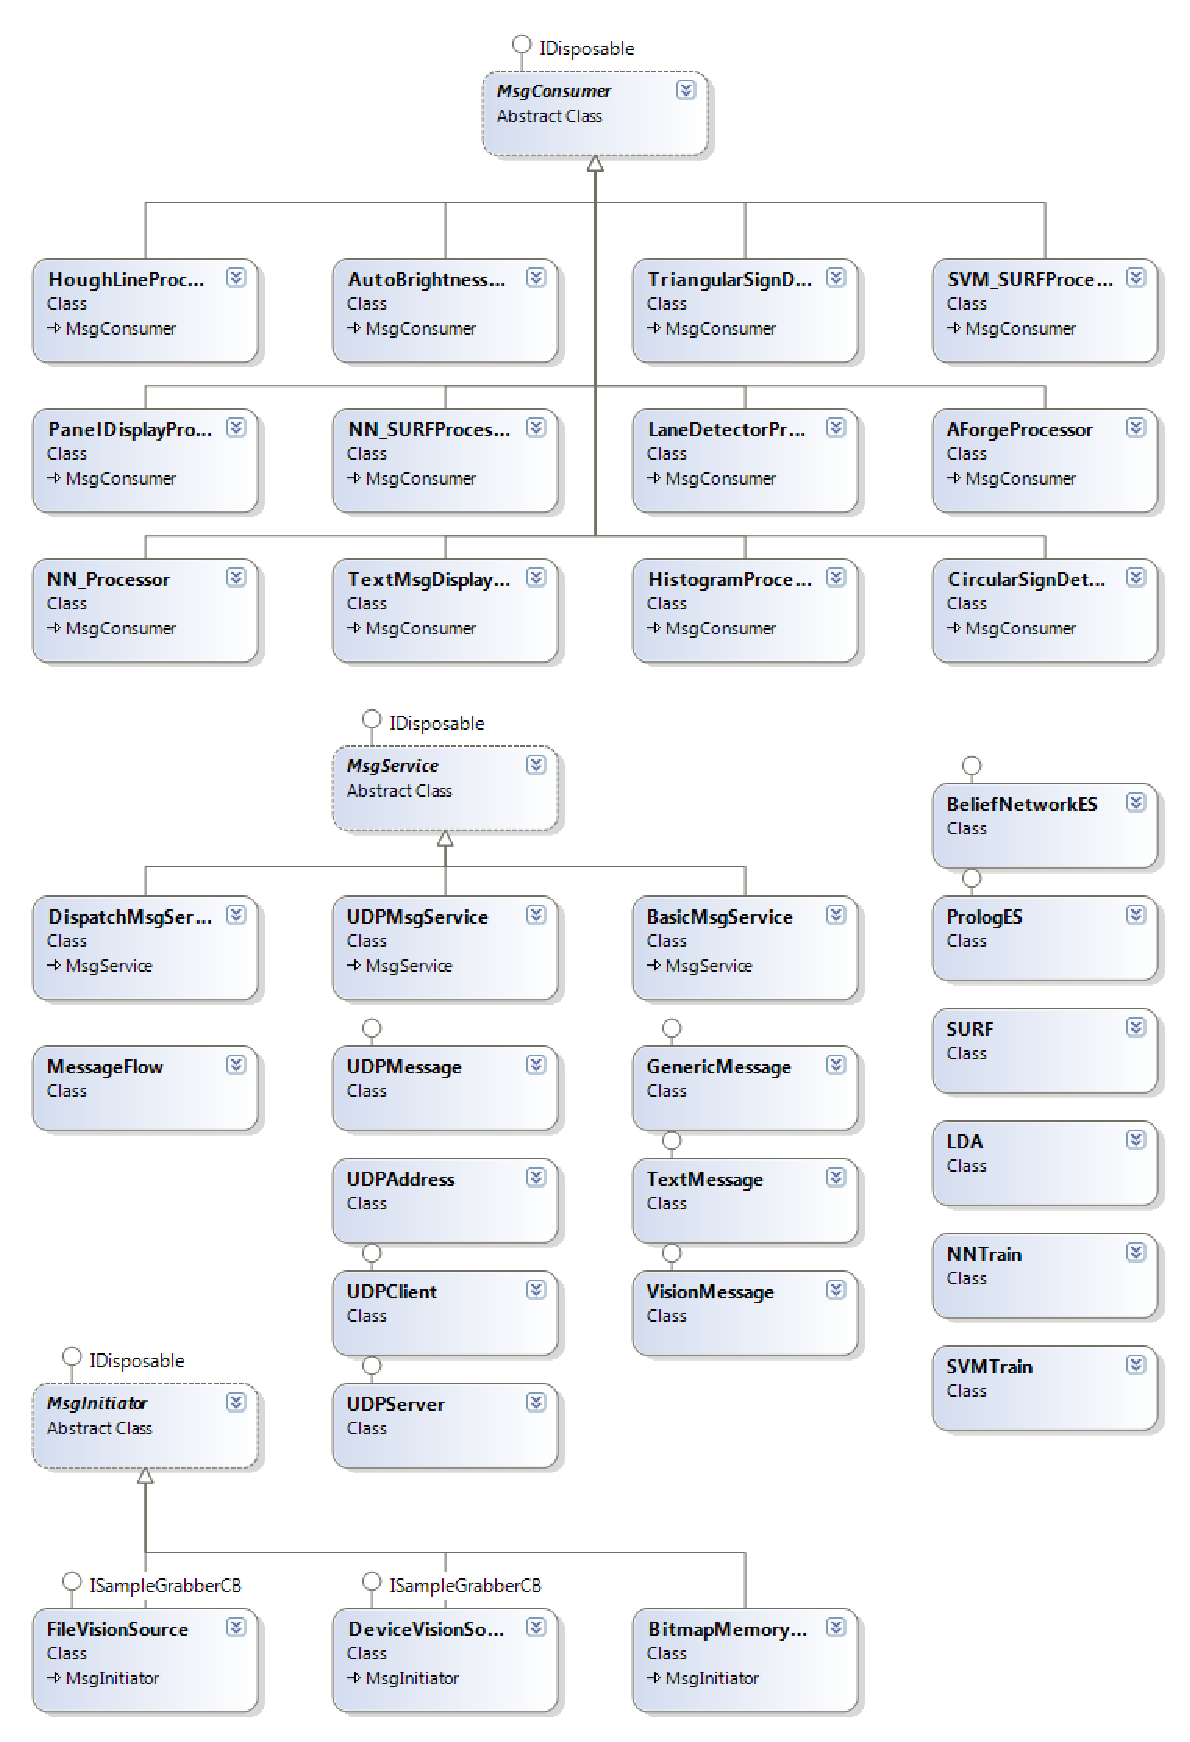
\includegraphics[width=140mm]{img/cdapp.eps}
\caption{ADES class hierarchy diagram.}
\label{fig:cdapp}
\end{center}
\end{figure}

\subsection{Class Reference for BOUNLib Namespace}
%%%%%%%%%%%%%%%%%%%% APIDOC %%%%%%%%%%%%%%%%

The BOUNLib.Processors.AForgeProcessor class is used as a generic processor for utilizing the AForge image library features.
This class inherits Messaging.MsgConsumer. The public member functions of this class are as follows.
\begin{itemize}
\item override void consumeMessage (IMessage message, int msgID): Consumes the provided message. 
\end{itemize}

The Processors.AutoBrightnessProcessor class is used as an automatic brightness correction processor.
This class inherits Messaging.MsgConsumer. The public member functions of this class are as follows.
\begin{itemize}
\item override void consumeMessage (IMessage message, int msgID): Consumes the provided message. 
\end{itemize}

The Messaging.BasicMsgService class simply transfers the acquired message to the target object.
This class inherits Messaging.MsgService. The public member functions of this class are as follows.
\begin{itemize}
\item override void sendMsg (IMessage msg): Send message to the target. 
\end{itemize}

The ES.BeliefNetworkES class is used as the Belief Networks based ES implementation.
This class inherits ES.ExpertSystems. The public member functions of this class are as follows.
\begin{itemize}
\item string init (params object[] esParams): Initializes the expert system. 
\item string assertFact (params object[] esParams): Fact assertion. 
\item string retractFact (params object[] esParams): Fact retraction. 
\item string[] query (params object[] esParams): Violation query feature. 
\item void setThreshold (double threshold): The violation threshold setter for driver aggressiveness. 
\item double getThreshold (): Violation threshold getter. 
\end{itemize}

The Sources.BitmapMemoryVisionSource class reads the vision information from memory.
This class inherits Messaging.MsgInitiator. The public member functions of this class are as follows.
\begin{itemize}
\item override void start (): Starts the information flow. 
\item override void stop (): Stops the information flow. 
\end{itemize}

The static ToolBox.ByteTools class is used for various byte operations. 
The public member functions of this class are as follows.
\begin{itemize}
\item static int intToByteArr (int data, byte[] outBuf, int pos): Converts integer to byte array. 
\item static int byteArrToByteArr (byte[] inBuf, byte[] outBuf, int pos): Copies a subarray of a byte array. 
\item static int intFromByteArr (byte[] inBuf, int pos): Extracts integer from byte array. 
\item static byte[] byteArrFromByteArr (byte[] inBuf, int pos, int size): Returns byte array from a subarray of a byte array. 
\item static byte[] BmpToBytes (Bitmap bmp, PixelFormat pf): Gets byte array from Bitmap. 
\item static Bitmap BytesToBmp (byte[] bmpBytes, int bmpWidth, int bmpHeight, PixelFormat pf): Constructs Bitmap from byte array. 
\item static PixelFormat bppToPixelFormat (int bpp): Bits per pixel to PixelFormat. 
\item static int pixelFormatToBPP (PixelFormat pf): PixelFormat to bits per pixel integer. 
\item static void imageCoM (Bitmap bmp, ref int com\_x, ref int com\_y): Center of Mass calculation for an image. 
\end{itemize}

The Processors.CircularSignDetectorProcessor class is used as a processor for detecting circular signs.
This class inherits Messaging.MsgConsumer. The public member functions of this class are as follows.
\begin{itemize}
\item override void consumeMessage (IMessage message, int msgID): Consumes the provided message. 
\end{itemize}

The NET.ImageFilters.ColorLabelFilter class is used as a custom AForge filter for color labeling.  

The static Constants class contains options for processors.  
The public member functions of this class are as follows.
\begin{itemize}
\item static float getAngle (int X1, int Y1, int X2, int Y2): Gets angle with atan(X2-X1/Y2-Y1). 
\item static double DIST (int x1, int x2, int y1, int y2): Euclidean distance.
\item static double DIST (Point p1, Point p2): Euclidean distance. 
\item static double MAX (double[] inArr, ref int idx): Gets MAX of array. 
\item static double MIN (double[] inArr, ref int idx): Gets MIN of array. 
\item static double getColorValForLabeling (Color clr): Arranges labeling color. Static Public Attributes
\item static string base\_folder: The base folder definition for training files and system outputs. 
\item static short IMAGE\_WIDTH: The width of the image. 
\item static short IMAGE\_HEIGHT: The height of the image.
\end{itemize}

The ToolBox.CRC8Calc class is used as a Class for calculating CRC8 checksums.

The Sources.DeviceVisionSource class reads the vision information from a connected camera.
This class inherits Messaging.MsgInitiator. The public member functions of this class are as follows.
\begin{itemize}
\item override void Dispose (): Release everything. 
\item override void start (): Starts the information flow. 
\item override void stop (): Stops the information flow. 
\end{itemize}

The Messaging.DispatchMsgService class creates a copy of the acquired message for all registered target objects.
This class inherits Messaging.MsgService. The public member functions of this class are as follows.
\begin{itemize}
\item override void sendMsg (IMessage msg): Send message to the target. 
\end{itemize}

The ES.ExpertSystems Interface should be used by the expert system implementations
Inherited by ES.BeliefNetworkES, and ES.PrologES.
The public member functions of this class are as follows.
\begin{itemize}
\item string init (params object[] esParams): Initializes the expert system. 
\item string assertFact (params object[] esParams): Fact assertion. 
item string retractFact (params object[] esParams): Fact retrection. 
\item string[] query (params object[] esParams): Violation query feature. 
\item void setThreshold (double threshold): The violation threshold setter for driver aggressiveness. 
\item double getThreshold (): Violation threshold getter. 
\end{itemize}

The static NET.Toolbox.FileTools class is used for the file operations. 
The public member functions of this class are as follows.
\begin{itemize}
\item static List of type FileInfo getTrainingFiles (ref int class\_count): Gets training files for NN and SVM. 
\item static void binarySerialize (String filename, object o): Writes a binary file to disk. 
\item static object binaryDeserialize (String filename): Reads a binary file from disk. 
\end{itemize}

The Sources.FileVisionSource class reads the vision information from video file.
This class inherits Messaging.MsgInitiator.The public member functions of this class are as follows.
\begin{itemize}
\item override void Dispose (): Release everything. 
\item override void start (): Starts the information flow. 
\item override void stop (): Stops the information flow. 
\end{itemize}

The Messages.GenericMessage class is used as the basic message format. All messages can be converted to this type for serialization purposes.
This class inherits Messages.IMessage.

The Processors.GeoTransChromosome class is used as the genetic algorithm processing class. 

The static Globals class contains global options for logging.  
The public member functions of this class are as follows.
\begin{itemize}
\item static void init (): Intializes the options with default values. 
\end{itemize}

The Processors.HistogramProcessor class finds the histogram of the captured image for improing the binarization process.
This class inherits Messaging.MsgConsumer. The public member functions of this class are as follows.
\begin{itemize}
\item override void consumeMessage (IMessage message, int msgID): Consumes the provided message. 
\end{itemize}

The Processors.HoughLineProcessor class is used as the Hough line processor for classical lane detection method.
This class inherits Messaging.MsgConsumer. The public member functions of this class are as follows.
\begin{itemize}
\item override void consumeMessage (IMessage message, int msgID): Consumes the provided message. 
\end{itemize}

The Messages.IMessage Interface is the messaging interface implemented by message classes.
Inherited by Messages.GenericMessage, Messages.TextMessage, \\
Messages.UDPMessage, and Messages.VisionMessage.

The Processors.LaneDetectorProcessor class is used as the  MHT and HMM base lane detector processor.
This class inherits Messaging.MsgConsumer. The public member functions of this class are as follows.
\begin{itemize}
\item override void consumeMessage (IMessage message, int msgID): Consumes the provided message. 
\end{itemize}

The NET.ImageFilters.LaneFilter class is used as a custom AForge filter for lane detection. 

The NET.Toolbox.LDA class is used for the LDA Calculation from training files. 

The ToolBox.Logger class is used as statistics logger. 

The Messaging.MessageFlow class is used as the main message flow binding object.
The public member functions of this class are as follows.
\begin{itemize}
\item void addConsumer (MsgConsumer item): Register consumers. 
\item void addInitiator (MsgInitiator item): Register sources. 
\item void startFlow (): Triggers the sources to start. 
\item void stopFlow (): Stops the flow. 
\end{itemize}

The Messaging.MsgConsumer class is used as the interface definition for processor classes.
Inherited by Processors.AForgeProcessor, Processors.AutoBrightnessProcessor, \\
Processors.CircularSignDetectorProcessor, Processors.HistogramProcessor, \\
Processors.HoughLineProcessor, Processors.LaneDetectorProcessor, \\
Processors.NN\_Processor, Processors.NN\_SURFProcessor, Processors.PanelDisplayProcessor, \\
Processors.SVM\_SURFProcessor, Processors.TextMsgDisplayProcessor, and \\
Processors.TriangularSignDetectorProcessor.
The public member functions of this class are as follows.
\begin{itemize}
\item Type getMsgType (): Returns the message type that the processor handles. 
\item abstract void consumeMessage (IMessage message, int msgID): Consumes the provided message. 
\end{itemize}

The Messaging.MsgInitiator class is used as the interface definition for source classes.
Inherited by Sources.BitmapMemoryVisionSource, Sources.DeviceVisionSource,
and Sources. FileVisionSource. The public member functions of this class are as follows.
\begin{itemize}
\item abstract void start (): Starts the information flow. 
\item abstract void stop (): Stops the information flow. 
\end{itemize}

The Messaging.MsgService class is used as the base message service class.
Inherited by Messaging.BasicMsgService, Messaging.DispatchMsgService, and \\
UDPServices.UDPMsgService. The public member functions of this class are as follows.
\begin{itemize}
\item abstract void sendMsg (IMessage msg): Send message to the target. 
\item virtual void receiveMsg (byte[] msg): Receive message from source. 
\end{itemize}

The Processors.NN\_Processor class is used as the sign classification processor uses NN based on grid based features.
This class inherits Messaging.MsgConsumer.
The public member functions of this class are as follows.
\begin{itemize}
\item override void consumeMessage (IMessage message, int msgID): Consumes the provided message. 
\end{itemize}

The Processors.NN\_SURFProcessor class is used as the sign classification processor uses NN based on SURF features.
This class inherits Messaging.MsgConsumer. The public member functions of this class are as follows.
\begin{itemize}
\item override void consumeMessage (IMessage message, int msgID): Consumes the provided message. 
\end{itemize}

The NET.Toolbox.NNTrain class is used for the neural network training process.

The ES.PrologES class is used as Prolog based ES implementation.
This class inherits ES.ExpertSystems. The public member functions of this class are as follows.
\begin{itemize}
\item string init (params object[] esParams): Initializes the expert system. 
\item string assertFact (params object[] esParams): Fact assertion. 
\item string retractFact (params object[] esParams): Fact retrection. 
\item string[] query (params object[] esParams): Violation query feature. 
\item void setThreshold (double threshold): The violation threshold setter for driver aggressiveness. 
\item double getThreshold (): Violation threshold getter. 
\end{itemize}

The NET.ImageFilters.SignFilter class is used as a custom AForge filter for sign detection. 

The static ToolBox.Statistics class contains statistics functions.
The public member functions of this class are as follows.
\begin{itemize}
\item static double GetVariance (int[] data): Get variance. 
\item static double GetStdev (int[] data): Get standard deviation. 
\end{itemize}

The NET.Toolbox.SURF class is used as the OpenSURF integration. 

The Processors.SVM\_SURFProcessor class is used as the sign classification processor uses SVM based on SURF features or grid based features.
This class inherits Messaging. MsgConsumer. The public member functions of this class are as follows.
\begin{itemize}
\item override void consumeMessage (IMessage message, int msgID): Consumes the provided message. 
\end{itemize}

The NET.Toolbox.SVMTrain class is used for the SVM training process. 

The Messages.TextMessage class is the text based information provided by the source objects.
This class inherits Messages.IMessage.

The Processors.TriangularSignDetectorProcessor class is used as the processor for detecting triangular signs.
This class inherits Messaging.MsgConsumer. The public member functions of this class are as follows.
\begin{itemize}
\item override void consumeMessage (IMessage message, int msgID): Consumes the provided message. 
\end{itemize}

The UDPServices.UDPAddress class is used for UDP connection address definition. 

The UDPServices.UDPClient class is used for UDP client implementation. 

The Messages.UDPMessage class carries information in distributed deployments of the processors and source classes.
This class inherits Messages.IMessage.

The UDPServices.UDPMsgService class is used as the UDP Messaging service.
This class inherits Messaging.MsgService.Classes. The public member functions of this class are as follows.
\begin{itemize}
\item override void sendMsg (IMessage msg): Send message to the target. 
\end{itemize}

The UDPServices.UDPServer class is used as the UDP server implementation. 

The Messages.VisionMessage class is used as the basic image information from the source objects.
This class inherits Messages.IMessage.

%%%%%%%%%%%%%%%%%%End Of Apidoc %%%%%%%%%%%%%%%%%%%%%%%%%%%

\section{SOFTWARE DEVELOPMENT METHODOLOGY}
Since the ADES project is developed by a team of engineers, basic software development tools and methods are applied. The most important component of these tools is the SVN repository which keeps the latest versions and all history of the codes. The svn repository of the project can be accessed via \textit{http://robot.cmpe.boun.edu.tr/svn/ADES/}. Since this is a restricted site, the authorization requests should be submitted to the project administrators. The details about the SVN can be accessed at \textit{http://subversion.apache.org/}.

Another tool used during the development of the project is Redmine, which is a flexible project management web application. Redmine is open source and released under the terms of the GNU General Public License v2 (GPL). Detailed information about the Redmine can be found in \textit{http://www.redmine.org}.

\bibliographystyle{style/fbe_tez_v11}
\bibliography{thesis}	

\end{document}
